%\documentclass[letter]{article}
\documentclass[letter,12pt]{article}
\usepackage[letterpaper,right=1in,left=1in,top=1in,bottom=1in]{geometry}

\usepackage{hyperref}
\usepackage{url}
\usepackage[pdftex]{graphicx}
\usepackage[longnamesfirst, sort]{natbib}\bibpunct[]{(}{)}{,}{a}{}{;}
\usepackage{arydshln}
\usepackage{amsmath}

\usepackage{rotating}
\usepackage{pdflscape}

\newcommand{\mc}{\multicolumn}

\graphicspath{{../graphs/}}
%\graphicspath{{graphs/}}

\begin{document}

\title{The Effects of Automated Redistricting and Partisan Strategic Interaction on Representation: \\ 
       The Case of Mexico\thanks{Paper prepared for delivery at the Annual Meeting of the American Political Science Association, Washington, DC, August 2014. We thank the Federal Electoral Institute (IFE) and the Federal Voter Registry (RFE). Special thanks to IFE's Cartography Department for sharing their experience with automated redistricting since 1996 and most of the data we analyze. We also acknowledge the support from the Asociaci\'on Mexicana de Cultura A.C.\ and CONACYT for this work.}}
\author{Micah Altman {\small \url{escience@mit.edu}} \\
        Eric Magar {\small \url{emagar@itam.mx}} \\
        Michael McDonald {\small \url{michael.mcdonald@ufl.edu}} \\  %\\ University of Florida, Gainesville\\
        Alejandro Trelles {\small \url{lat44@pitt.edu}}
      }
\date{\today}
\maketitle



\begin{abstract}
%Abstract Version 1
\noindent In the U.S.\ redistricting is deeply politicized and often synonymous with gerrymandering ---the manipulation of boundaries to promote the goals of parties, incumbents, and racial groups. In contrast, Mexico's federal redistricting has been implemented nationwide since 1996 through automated algorithms devised by the electoral management body (EMB) in consultation with political parties. In this setting, parties interact strategically and generate counterproposals to the algorithmically generated plans in a closed-door process that is not revealed outside the bureaucracy. Applying geospatial statistics and large-scale optimization to a novel dataset that has never been available outside of the EMB, we analyze the effects of automated redistricting and partisan strategic interaction on representation. Our dataset comprises the entire set of plans generated by the automated algorithm, as well as all the counterproposals made by each political party during the 2013 redistricting process. Additionally, we inspect the 2006 map with new data and two proposals to replace it towards 2015 in search for partisan effects and political distortions. Our analysis offers a unique insight into the internal workings of a purportedly autonomous EMB and the partisan effects of automated redistricting on representation.

% Comment [Eric and Alejandro]: Two alternative abstract versions bellow.
% Comment [Alejandro]: Given the direction the paper is taking, I wrote a new abstract and moved the previous version to option 3. The floor is open for comments, suggestions or modifications...

% Abstract Version 2:
% Mexico's federal redistricting has been implemented nationwide since 1996 through automated algorithms devised by the electoral management body (EMB) in consultation with political parties. In this setting, parties interact strategically and generate counterproposals to plans in a closed-door process that is not revealed outside the bureaucracy.The way that redistricting has played out so far in Mexico raises a number of questions: Were the adopted redistricting criteria politically neutral? Were the plans produced algorithmically, in fact, optimal with respect to the selected criteria? How did partisan counterproposals differ from the bureaucratic solution? What influence did parties have on the final proposed plan? Can automated and partisan interactive  models  generate relatively fair and unbiased plans? We address these questions by applying geospatial statistics and large scale optimization to a novel dataset that comprises the entire set of plans generated by the automation algorithm and all plans proposed by political parties during the 2013 redistricting process. Our findings offer a unique insight into the internal workings of a purportedly autonomous EMB and the partisan effects of automated redistricting on representation.

%Abstract Version 3:
%In the U.S. redistricting is deeply politicized and often synonymous with gerrymandering ---the manipulation of boundaries to promote the goals of parties, incumbents, and racial groups. In contrast, starting in 1996, Mexico's federal redistricting has been implemented nationwide through an automated algorithm devised by the electoral management body (EMB) in consultation with political parties. The system purports to produce plans that are optimal. However, until recently, Mexico's redistricting process has been closed to both public participation and inspection. We inspect new data of the 2006 map and two proposals to replace it towards 2015 in search for partisan effects and political distortions. Unlike analysis of the votes-to-seats conversion at the national-level, state-level data reveal no evidence of systematic party bias. What bias there is in federal districts is of another kind, a big bonus for larger parties (or vote responsiveness) typical of plurality rule in single-member districts. Since most states distribute few seats each, the large party bonus of states' federal districts doubles the estimate with national data. Since the PRI is the largest party in most states, it receives a substantial seat bonus.

% Comment [Micah]: Last two sentences of version 3 are unclear. Reword? 
\end{abstract}

% Comment [Eric]: Possible argument for the presentation.
% Expert committees can remove partisan bias from redistricting.
% Mexico's process allows parties to respond. Offers leverage to infer party preferences and degree of influence. 
% Analysis of party bias and responsiveness informs this, directly. 

A fundamental principle of democratic governance is the will of the people is translated into public policy. Usually, electoral institutions serve the purpose of translating the peoples' will, expressed by their votes, into the selection of representatives, who enact policies. In redistricting --- the periodic drawing of electoral boundaries, ostensibly to achieve seemingly apolitical goals such as balancing districts' populations --- the causal chain can be reversed. The drawing of new electoral boundaries may allocate voters to districts in ways that affect the number of legislative seats parties are expected to win, the careers of incumbents, and representation for racial groups. With so much at stake, scholars have found the redistricting process can distort representation, through an eponymous strategy known as gerrymandering \citep{mayhew1974vanishingMg,cox.katz.2002,erikson1972malapportionment,engstrom2006redisttrictApsr}. Some state governments have sought to remove the opportunity for politicians to engage in gerrymandering by shifting redistricting authority from state legislatures to commissions; although some commissions' rules and membership continue to produce highly politicized outcomes, while others less so \citep{mcdonald.CommVsLegisRedistrict2004,trelles.mtz.polygob2012}. Mexicans similarly decided to overcome this challenge by delegating redistricting authority to the Federal Electoral Institute (IFE), an independent election management board (EMB) created in 1990. Mexico has innovated beyond the U.S. by employing self-tailored automated algorithms to find redistricting plans deemed optimal on \emph{a priori} criteria, and for political parties to react by offering counter-proposals \citep{trelles.mtz.polygob2012}. Here, we examine the extent to which technocrats have supplanted politicians \citep{lujambio.vives.2008} by analyzing a novel dataset describing partisan interaction within IFE in the 2013 redistricting process.

% Comment [Mike] rewrote the first paragraph to raise the big picture before getting into the redistricting weeds
% Comment [Eric] Mike's version looks good
% Comment [Alejandro] Agree, looks good... 

Despite that electoral officials may claim to be politically neutral, scholars find the rules by which electoral management bodies operate may not constrain political manipulation \citep{lijphart.1990,rossiter.etal.1997,estevez.magar.rosas.2008}. Furthermore, criteria may embody subtle second order biases that produce a predictable political outcome \citep{parker.1990}. Rather than removing political bias, redistricting by commission may perpetuate it in a different guise. In particular, IFE conducts redistricting behind closed doors, without public scrutiny, much less public participation \citep{trelles.mtz.tesisItam.2007}.\footnote{The lack of information in previous redistricting rounds, even within the EMB, generated non-functional districts. In 1996 and 2004, for instance, electoral commissioners received complains --- from several local IFE commissions and party representatives in states like Sonora and Chihuahua --- arguing that they where not allowed to participate in the redistricting process and that several districts, despite being "optimal," where splitting communities or had major geographical accidents making them dysfunctional for organizational and campaign purposes \citep{trelles.mtz.tesisItam.2007}.} The media and public are provided insufficient information to assess if the final plan embodies political mischief --- for example, how the plan produced by automation methods differs from the final plan --- before the new plan is formally adopted by IFE's Council General and takes effect.

% comment [Mike] who adopts the plan? Does the legislature formally vote to approve IFE's proposed plan? If IFE's word is final, strike "formally adopted and"
% Comment [Eric] Legislators appoint IFE's Council General (and have means to control them ex-post); the Council General approves the new map. I have added this in the last sentences. 
% Comment [Alejandro]: I took care of Mike's comment and Eric's footnote...

In 2013, as in 1996 and 2005, IFE employed an algorithmic redistricting process based upon criteria agreed amongst IFE's electoral commissioners before plans were drawn. IFE used the 2005 algorithm (a simulated annealing combinatorial optimization heuristic) with the same four input parameters (population balance, compactness, municipal integrity and traveling time), but with a slightly re-weighted overall scoring function to optimize \citep{trelles.mtz.tesisItam.2007,acuerdoife2013}. As in 2005, the base geography was modified so that the algorithm could not partition minority municipalities and 25 districts where created with at least 40\% of indigenous population. 

% comment [Mike] I recall the optimization algorithm was bee hive, not simulated annealing. Might cite the original documentation here to give credit to the mathematicians who programmed the algorithm.

% comment [Alejandro]: In 1996 the algorithm was known within IFE as "heuristic" (it was an algorithm that aggregated sections from West to East and from North to South in each state balancing population and trying not to split municipal administrative divisions (traveling time, compactness and minority districts were not in the picture yet); in 2005, IFE used the simulated annealing algorithm for the first time (a heuristic with a cost function that aggregated sections departing from a randomly chosen seed that evaluated results under a high-low "temperature" dynamic. It was in this round (2005) that the 4 criteria that we mention were introduced for the first time; In 2013, IFE decided to use again the simulated annealing algorithm and the same 4 criteria weighted slightly different and they explored the possibility of complementing the simulated annealing with bee hive optimization. However, according to Miguel, they decided not to use bee hive optimization because the cost function was not improved significantly. 

The last redistricting process towards the 2015 election offers an opportunity to assess the robustness of Mexico's redistricting process. For the first time, IFE created a web-based map sharing tool, which allows us to analyze all redistricting plans formally introduced throughout the process. A large number of plans were produced, more than in any previous redistricting, as IFE invited two sets of institutional actors to participate in the process: the seven national parties represented in the National Surveillance Commission (NSC) and the same seven parties represented in each of the 32 state-based Local Surveillance Commissions (LSC). IFE’s Technical Redistricting Committee enabled strategic interaction between entities by allowing them to observe counter-proposals formulated by other parties through the platform. Observations and counter-proposals took place in the first and second --- out of three --- stages of the process.\footnote{The idea of partisan interaction was introduced in the International Redistricting Seminar celebrated at IFE in Mexico City in November 2012. IFE had allowed parties to formulate observations in 1996 and 2005, but no interaction platform existed so that parties could observe what others were proposing. The authors of this paper introduced the idea during the presentation of the Public Mapping Project Mexico (www.publicmapping.org), an open source web based platform that allows citizens and parties to analyze redistricting scenarios, observe what other users are proposing, and formulate counterproposals in order to optimize the criteria established by the legal framework and allow the authority in charge of redistricting to automatically rank and evaluate counterproposals.} 

% Comment [Eric] I adopted the convention of naming maps by the first election they were or would have been in use. I changed 2013 with 2015 in the start of the previous paragraph. 

% Comment [Alejandro]: I eliminated the "that we were granted access to" from the paragraph above because this is was not official and I do not want to overexpose our friends at IFE (there is no problem if we mention this in a panel informally, but I would like to be cautions in manuscripts)...

In the end, despite consensus within party representatives at the EMB to endorse the final plan (they actively participated in the process), unexpected partisan resistance in the three major national party headquarters (PAN, PRI and PRD) stalled adoption of IFE's final plan and ushered in a set of reforms to the Mexican electoral system in early 2014. The way that redistricting has played out so far in Mexico and the last set of electoral reforms --- specially the reintroduction of legislative reelection starting in 2015 --- raise a number of questions: Are the adopted redistricting criteria politically neutral? Were the plans produced algorithmically optimal with respect to the selected criteria? How did partisan counter-proposals differ from the bureaucratic solution? What influence did parties have on the final plan? 

In this work we answer these questions and assess Mexico's redistricting process in search of partisan effects on representation by inspecting data that has never been available outside of the Mexican government. It comprises the machine generated plans and two rounds of strategic counter-proposals made by political parties. We focus on the 300 single-member district (SMD) seats in the federal chamber of deputies (out of 500 seats).\footnote{Since no boundary lines are drawn for the compensatory 200 proportional representation (PR) seats, we do not analyze these seats.} 

\section{Automated Redistricting and Partisan Interaction}

Mexico adopted a mixed-member electoral system for the lower house of Congress in 1978. In the first election, three hundred single-member districts were drawn to elect three-fourths of the chamber by plurality rule. Districts were not redrawn until 1996, coinciding with the first free and fair national election in 1997 \citep{lujambio.vives.2008,trelles.mtz.tesisItam.2007}. A second redistricting occurred in 2005, and a third (failed to be adopted) in 2013. In the following lines we refer to district maps by the first year they were in use, not by the actual year they were drawn.\footnote{Despite maps were actually drawn in 1978, 1996, 2005, and 2013, we will refer to them as 1979, 1997, 2006 and 2015, respectively. The last case (2015) is hypothetical.}

% comment [Mike] I'm sure the "first free and fair election" is common knowledge within Mexico, but can we provide a cite? 
% comment [Eric] DONE

In 1997, for the first time, IFE implemented a redistricting process whereby computer-generated plans informed the national political parties represented at the EMB \citep{trelles.mtz.tesisItam.2007}.Since then, the process involves three stages: 1) the apportionment of the 300 single member districts into the 32 states; 2) the development and implementation of an automated optimization algorithm; and 3) the analysis of the automated generated maps by a technical committee and an in-door discussion where political parties are able to suggest modifications to the plans in two different stages. 

The first stage starts with the apportionment of congressional seats to the 32 states based solely on population.\footnote{One "state" is the Federal District for Mexico City, which is similar to Washington, D.C.} As in the U.S., no district crosses state boundaries and all districts must be contiguous. In the next section we discuss this method and describe its effect on representation. In sharp contrast to the U.S.\ \citep{szpiro.numbersRule.2010}, little, if any debate about alternative apportionment methods has been undertaken. 

In the second stage, an optimization model to construct congressional districts from the base-geography --- states' \emph{electoral \emph{secciones}} --- is devised. Mexico is comprised of more than 66,000 \emph{secciones}, which are analogous to U.S.\ census tracts. Median \emph{secci\'on} population in the 2010 census was 1,280 persons, with a maximum at 79,232. Similar to the U.S.\ Voting Rights Act's guarantees for minority representation, \emph{municipios} --- the smallest elected offices, similar to counties in the U.S.\ --- with sizable indigenous populations cannot be partitioned. 

% comment [Mike] I think it would be better to use the Spanish word for sections (italicized) since the English word "section" can be ambiguous. Same goes for municipality.
% [Eric] I agree and have changed them throughout the MS.

The optimization model has been refined in each redistricting round. In the 2015 redistricting process, the algorithm aggregated \emph{secciones} into congressional districts starting from a randomly selected seed in each state and then weighted and rewarded differently the following variables trying to \emph{minimize} a cost function composed of the following components: 1) population balance (allowing up to 15\% deviations across districts), 2) the preservation of municipal boundaries, 3) the minimization of travelling times within the district, and 4) district compactness.\footnote{Population was assigned 40\% of the overall cost function score, municipal boundaries 30\%, traveling times 20\%, and  compactness 10\%.} After thousands of iterations, a map minimizing the cost function of the algorithm is proposed and it is commonly known as the first scenario. In the latest redistricting process, the first scenario was presented on July 17, 2013 for discussion.

% comment [Eric] It would seem that the cost function does not seem to minimize population imbalance outside the +/-15% margin. It seems to have a discontinuity: imbalance outside the margin is increasingly penalized, but no change in cost occurs once the district is inside the tolerance range. Is this correct? If so, the sentence above might need clarification. 

% comment [Alejandro]: No, it is not correct. A lower population imbalance will always have a positive impact on the cost function (it will decrease the cost), even when two scenarios are under the 15% threshold. I am not sure how to rephrase the paragraph to reflect this without making the sentence too confusing... 

The third stage begins once the first scenario has been formally presented by IFE's technical committee --- appointed by the the EMB's Genral Council --- and distributed to the parties. It involves two rounds where technical experts comment on the maps and political parties observe and suggest modifications to the maps.\footnote{This stage took approximately 4 months. It began in July 2013 and concluded in October 2013.} Amendments are proposed to the first scenario, and those that are adopted by the technical committee are then used as a starting point for another round of partisan observations to produce a second scenario. Parties are invited again to propose a second round of amendments and, once they have been analyzed and discussed by the technical committee again, a final plan is presented to the EMB's General Council to be formally approved.

% comment [Mike] Alejandro, please check this over for accuracy. I added text to describe the steps between the first and second scenario and the second scenario and the adopted plan.

% comment [Alejandro]: Done. Optimization just happens once, so I corrected the sentence... The same in line 146

It is at this stage where parties interact strategically with mapmakers, and other parties. Parties propose amendments to the computer-generated plans, but these amendments must improve the overall cost score to be considered for adoption. Table \ref{T:counterprops} summarizes the two rounds of amendments that took place in preparation for the 2015 map. The number of proposals increased significantly over previous redistricting, because the national EMB expanded participation to the state EMB counterparts, which provided the parties two channels to deliver simultaneous counter-proposals to the EMB. There were a total of 534 counterproposals made for the 2015 map (more than twice of the counterproposals made for the 1997 and 2006 maps). 236 counterproposals were made to the first scenario (157 from the LSC and 79 form the NSC) and 308 were made to the second scenario (139 by the LSC and 169 by NSC).

% Comment [Alejandro]: We might want to include table 1 and/or 3 in the word document shared previously by me on the G drive entitled "APSA2014Paper"...


Parties actively challenged proposed districts, making 75 counter-proposals each on average. Although we expected that all 7 parties would behave as rational self-interest maximizers and strategically make competitive counter-proposals to the first scenario, the right-of-center PAN was, by far, the most successful. Nearly half of their 82 proposals were accepted, compared to about one-fifth for the other major parties (PRI and PRD). Amendments originated in both national (7 parties at the National Surveillance Commission) and state level (same 7 parties represented at 32 Local Surveillance Commissions).\footnote{The full set of parties represented in each committee were PAN, PRI, PRD, PT, PVEM, MC and PNA.} Activity at the amendment stage was enhanced by the adoption of an internal web-based map-sharing tool, which standardized counter-proposals and enabled parties to observe each others' amendments --- improving information for strategic behavior. The final proposal for Council General approval was presented on October 15, 2013. In the midst of a major electoral reform that took place in December that year, the Council General, driven by the pressure of the three major parties (PAN, PRI and PRD), chose not to decide before the end of the year. The 2015 midterm election, it was soon after learned, would be held with significantly outdated districts. 

% Comment [Alejandro]: The idea of "rational self-interest maximizers and strategically make competitive counterproposals to the first scenario" comes from the previous draft APSA2014Paper (available in G drive) and it is a possible path we want to explore to complement this paper or for publications in the near future...
% comment [Mike] what is the "strategic dimension"? How can we quantify it?
% comment [Eric] I have changed to better information for strategic behavior. Developing the game seems beyond this paper, but may shed interesting results.

% Comment [Alejandro]: A way to quantify and contrast the "strategic dimension": If we put computers (or students, as we did with the PMP demo of the State of Mexico with Eric's class) to play the game and minimize the cost function (departing from the first scenario) and maximize their utilities (as if they were parties), we could model and find the equilibrium under strictly rational principles / behavior. This would be our anchor to compare what happened in real circumstances to what could have happened if agents had been "more strategic". If we did that exercise, I am pretty sure that, given historical electoral results and the PRI's favorable position in most states across the country, the PRI would be the party that is more likely to make the most "efficient" counterproposals (not the PAN) in the first and second rounds of counterproposals. An alternative way to quantify and compare efficient solutions, from the party perspective, would be to try to minimize the cost function, while maximizing the vote share for each party by including a fifth variable/criteria (party vote share) to the four criteria that are already being used by IFE. What would have happened if the PRI and PRD had been as efficient as PAN in making counterproposals? Again, I suspect that given the PRIs electoral advantage across states, they would be, by far, better positioned to make the most effective counterproposals because they would give the simulated annealing algorithm a wider margin to offer more efficient (lower cost function) solutions... 

\begin{table}
\begin{center}
  \begin{tabular}{lrrr|rrr|r}
    Party & national & state  & total 1st & national   & state  & total 2nd & Total \\ \hline
    PAN	  & 17/22    & 2/20   & 19/42     & 17/24      & 4/16   & 21/40  & 40/82 \\
    PRI	  & 0/0      & 2/28   & 2/28      & 8/30   & 6/26   & 14/56  & 16/84 \\
    PRD	  & 3/27     & 2/21   & 5/48      & 5/29   & 5/18   & 10/47  & 15/95 \\
    PT	  & 1/12     & 1/20   & 2/22      & 3/15   & 1/16   & 4/31   & 6/53 \\
    PVEM  & 0/0      & 1/20   & 1/20      & 7/28   & 3/17   & 10/45  & 11/65 \\
    MC    & 1/17     & 0/21   & 1/38      & 6/32   & 2/16   & 8/48   & 9/86 \\
    PNA   & 0/1      & 1/18   & 1/19      & 4/11   & 3/17   & 7/28   & 8/47 \\
    IFE   & 0/0      & 1/9    & 1/9       & 0/0    & 5/13   & 5/13   & 6/22 \\ \hline
    Total & 22/79    & 10/157 & 32/236    & 50/169 & 29/139 & 43/308 & 111/534 \\
  \end{tabular}
  \caption{Counter-proposals to the first and second scenarios at the National and Local Surveillance Committees. Denominator reports the number of counter-proposals made, numerator how many were adopted. Prepared by authors with information from the Federal Electoral Institute.}\label{T:counterprops}
\end{center}
\end{table}

% comment [Mike] changed PT total 1st from 2/32 to 2/22 and grand total from 32/236 to 32/226; likewise total PRD 12t and 2nd changed from 6/63 to 6/53 and grand grand total from 111/544 to 111/534

% comment [Alejandro]: changed the word proposal for scenario in Table 1 description (first line). Same thing in the paragraph bellow... SCENARIO = departing point; and PROPOSAL (or COUNTER PROPOSAL)  = a modification proposed by a party of IFE. 

We investigate how the 2015 redistricting process unfolded in Figure 1. For each of Mexico's thirty-two states we plot the overall score for each proposed redistricting plan (the value of the algorithm's cost function for the three scenarios are black points, numbered). The optimization objective is to produce a plan with the least cost, so plans with lower values are better than plans with higher values. The first scenario resulted from the optimization algorithm prior to party feedback, the second and third from party amendments. Colored points are party counteproposals to the second scenario, blue for the PAN, red for the PRI, yellow for the PRD, grey for the best offer by a minor party.\footnote{The same analysis for party reactions to the first proposal would reveal another interesting aspect of negotiation. A successful amendment in the first round sets the starting point for the optimization process towards the second round, and this might lend important proposal power. PAN was, by far, the most successful party in the first round.} Brown points represent two or more counter-proposals with equal scores, with one protruding petal for each plan. The cost function is expressed relative to the value of the second proposal. 

% comment [Alejandro]: Optimization just happens once, so I corrected the paragraph above...

%\begin{landscape}
\begin{figure}
\begin{center}
    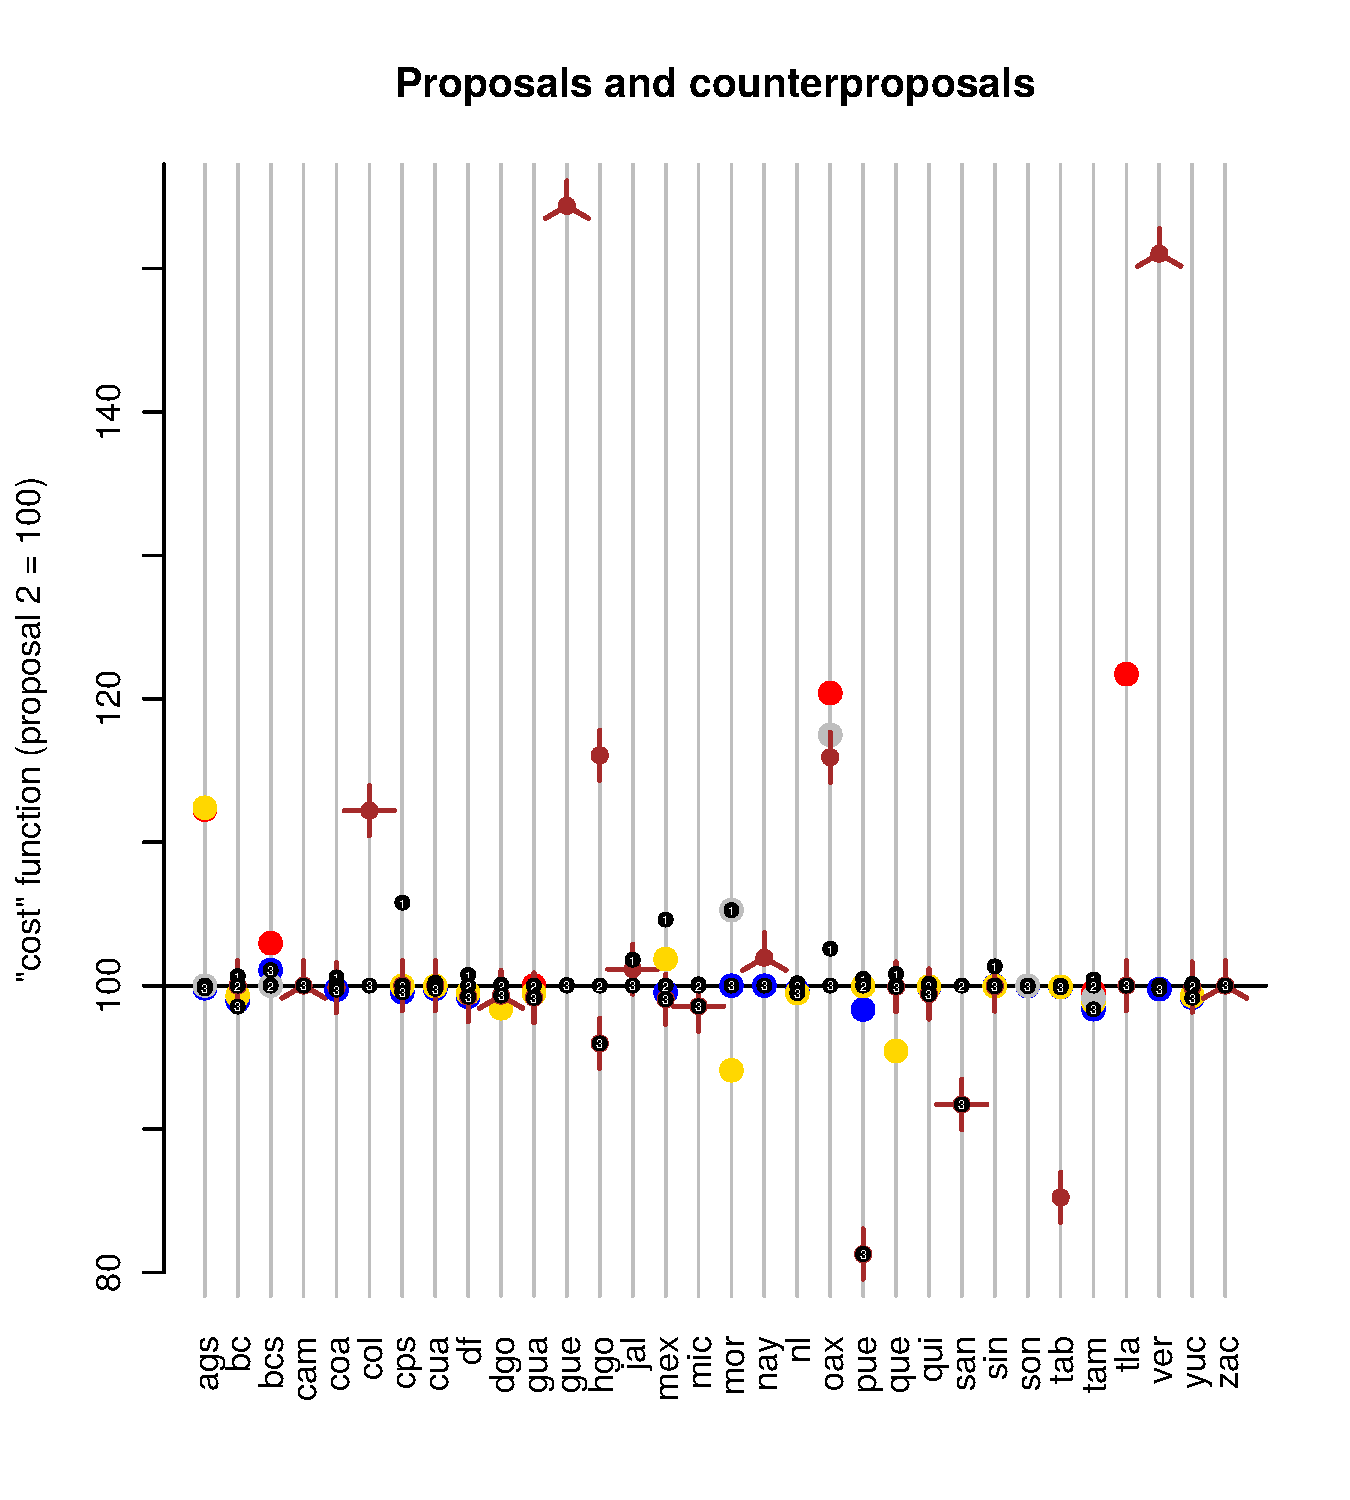
\includegraphics[width=\columnwidth]{propsAndCost.pdf} \\
  \caption{Map proposals towards 2015 by state. Black, numbered points indicate the value of the algorithm's cost function for the three map scenarios. The cost function is expressed relative to the value of the second proposal. Colored points are party counterproposals to the second proposal, blue for the PAN, red for the PRI, gold for the PRD, grey for the best offer by a minor party. Brown points report overlaps of two or more counter-proposals, one protruding petal for each overlap.}\label{F:propsAndCost}
\end{center}
\end{figure}
%\end{landscape}

In all but one state (Baja California Sur, BCS), the progression of scenarios is towards improving the cost function, as the third and final scenario has a lower score than either of the two prior scenarios. We observe numerous instances where humans "beat" the machine, by offering counter-proposals that improve the first scenario's score. These plans demonstrate how redistricting is a complex integer optimization problem where optimization algorithms can become stuck in local optima \citep{altman.mcdonald2011bard}. Where the adopted amendments to the first scenario improve the score greatly --- as is the case in Hidalgo (Hgo), Puebla (Pue) and San Luis Potos\'i (San) --- the second round of counterproposals fails to further improve the previous round given that the margin to make changes becomes narrower. We cannot know for certain if these final plans are the global optimum since the algorithm departed from a randomly chosen seed and redistricting is such a challenging optimization problem.

% comment [Mike] why did the Baja final plan score worse than the second plan? Is this a data entry error, or is something else at play?

% comment [Alejandro]: Optimization just happens once, so I corrected the paragraph above...I think there might have been something else at play, but I will definitely ask Miguel (and look at the parties comments, which we have in our G-drive). 

There are three instances where the PRD offered a counter-proposal improving upon the first scenario and all other amendments, but the amendment was rejected: Durango (Dgo), Morelos (Mor), and Quere\'taro (Que). Two identical plans proposed in Tabasco (Tab) similarly are the objectively best plans, but are rejected. In these three instances, a second round of partisan observations fails to find better plans. This provides further evidence of how automated algorithms are challenged by the complexities of redistricting. More importantly, the existence of these better plans demonstrates that politics is present in the process, likely to the detriment of the PRD.   

% comment [Mike] We should say more about the politics behind these three rejected PRD plans. Also, was the PRD one of the two parties proposing plans for Tabasco?

% comment [Eric] In Tabasco, the plans rejected were by PRI and a minor party (PVEM).

% comment [Alejandro]: We should talk about the politics behind this process in our next call and decide how we want to describe it. I can tell you my experience from 2005 and tell you about what Miguel told me of the 2013 process... In a nutshell, party representatives at IFE are not very "skilled" and they were not very efficient in terms of minimizing the cost function, while maximizing their electoral rent. They made cost winning proposals (like PAN), but where not very efficient maximizing votes. In other words, they lack expertise is big part of the explanation of inefficient outcomes. We should see them becoming more efficient in subsequent redistricting rounds (as they learn how to play this interactive game better with practice)! Most of the politics in the 2013 process was related to the apportionment stage (PRD was against redistrciting because their strong hold, Mexico City, lost a significant number of districts to the State of Mexico, a strong hold of the PRI), but it really did not have to do with things such as the criteria, how they were being wighted, the optimization algorithm or the two rounds of partisan counterproposals. I know, from very good sources, that there also was a major miss communication between party represenatatives at IFE and the parties national headquarters (this is specially true for PAN). Once the elite at the national headquarters did the math (analyzed the third scenario using electoral information), they started pressuring the General Council to postpone the approval of the plan (contrary to how their party representative was playing the game)... This explains why PAN was pressuring towards the suspension of the new map despite they won most of the counterproposals in the first and second stages.   

There are several proposals that have identical scores to the first scenario, and several instances where two proposals have identical scores. If two scenarios were tied, the technical committee would adopt the proposal that had lower cost values associated to the most relevant criteria --- population, followed by municipal integrity, traveling time and compactness at the end \citep{acuerdoife2013}. Further investigation may reveal subtle differences between these seemingly-similar plans, such as the assignment of two \emph{secciones} to different districts that has minimal changes on the overall score. We also observe numerous instances where parties propose plans that score worse than the first scenario. In many cases, as in 2005, parties decided --- even if the cost function of their counterproposal was higher than the departing scenario --- to present their plan and try to argue that their plan represented better specific communities or that responded better to geographical or socioeconomic characteristics not considered by the optimization algorithm.

% comment [Mike] when was the rule to reject worse scoring plans adopted? Was is adopted after counter-proposals to the first scenario were proposed? 

% comment [Eric] Rojano's data has lots of digits after the decimal point, so should be sensitive to seccion reaassignement. Parties must have played mostly with complete municipios, reaching the same solutions. Does this sound correct Alejandro?

% comment [Alejandro]: The answer is no Mike. This is a rule (rejecting worse scoring plans) established by the technical committee and it was socialized with all the parties prior to the creation of the first scenario (in 2005 and in 2013). This did not happen in 1996 because there was no "cost function" (for the function or for the major criteria). One of the major "improvements" in the 2005 redistricting process was that for the first time there was a score for the cost function, as well as a cost associated to each of the four criteria (population, compactness, municipal integrity and traveling time). If two scenarios were tied in the total cost function, the technical committee would have an inclination to select the proposal that had lower cost values associated to the most relevant criteria (the most important was usually the population component).  

In another key respect, all processes have remained opaque activities between electoral regulators and party representatives. New technology letting anyone interested, with little more than an Internet connection, see proposals, react, and improve them through crowd-sourcing or an open web based platform \citep{altman.mcdonald2011bard,Trelles.2015}, remains to be adopted. We observe evidence to suggest such transparency may not be welcome by all parties, as the PRD proposed objectively better plans that were never adopted.

% Comment [Alejandro]: Eric, could you please add to the citation in the paragraph above next to Altman and McDonald 2011, "Trelles Forthcoming." I understand you have them linked to Endnote, right? Thanks.

%Complete reference. Trelles, Alejandro. Forthcoming. Drawing Electoral Boundaries in Mexico: International Transparent Participative Mapping around the Globe. In The Weakest Links: Risks Arising during the Electoral Cycle, ed. Ferran  Martínez i Coma, Pippa Norris, and Richard W. Frank.  Oxford: Oxford University Press. 
% comment [Eric] DONE

% Comment [Eric]: Alejandro asked for a graph reporting proposals in terms of the cost function that IFE uses. Below is the best I could prepare... 

% comment [Mike] this graph is excellent! Thanks for producing it. I'll have to chew on it for takeaways [I've written some of this into text, but I'm keeping my original comments here]. Were these only counter-proposals to the second scenario? If proposals that would fare worse on the cost function are automatically rejected, why do we observe a fair number of proposals increasing the cost function, and presumably would be immediately rejected? (Note in bcs -- only -- the cost function increases between the second and third scenario!) Why do we see plans that improve the score rejected (mor, que, and tab)? Why do we see more than one party proposing plans with the same cost function? If these are the same plan, what is the value for more than one party proposing the same plan? Is there a way to tell if these plans are different plans, but happen to have the same score? Can we do a bias and responsiveness analysis to see if a party ever proposes a plan that works against them? I wonder if we can say something about the limits of optimization by providing the number of districts apportioned to each state. My guess is that the states with fewer plans that improve the cost function have a smaller number of districts (and thus the optimal plan is easier to discover).

% comment [Alejandro]: To answer Mike's question, I added the following text above "In many cases, as in 2005, parties decided --- even if the cost function of their counterproposal was higher than the departing scenario --- to present their plan and try to argue that their plan represented better specific communities or that responded better to geographical or socioeconomic characteristics not considered by the optimization algorithm". As I explained before, this tells us that parties are in a learning process (learning how to play this game) and sometimes they believe that arguments involving better representation could prevail over a cost function. This was extremely common in 2005, and I am sure it happened again in 2013. PRD is the party that usually has less technical resources and "skillful" personnel to defend their interests. This might explain their poor performance. The explanation of why "better cost function" plans where rejected by the committee is that there was some "margin" for the committee to evaluate if they would adopt a counterproposal. The cost function, for instance, could have improved because the traveling time was reduced, but the population balance increased slightly. In this example, the technical committee might have just decided to stay with an overall higher cost plan, but with a better population balance. This happened in 2005, and I would not be surprised if it happened again in 2013.  


\section{The Apportionment of Congressional Seats to States}

The Hamilton method of largest remainders is used for apportionment of Mexico's national legislative seats to the states \citep[][:10]{balinskiYoung2001FairRep}. The quota $Q$ (or price) of a seat is the nation's population divided by 300, the number of seats since 1979. A first allocation is made by dividing each state's population by $Q$, rounded down. Unallocated seats, if any, are awarded to states with largest fractional remainders. By law, no state can have fewer than 2 seats (Colima and Baja California Sur fell in this category in early apportionment rounds.) 

\begin{figure}
\begin{center}
  \begin{tabular}{cc}
    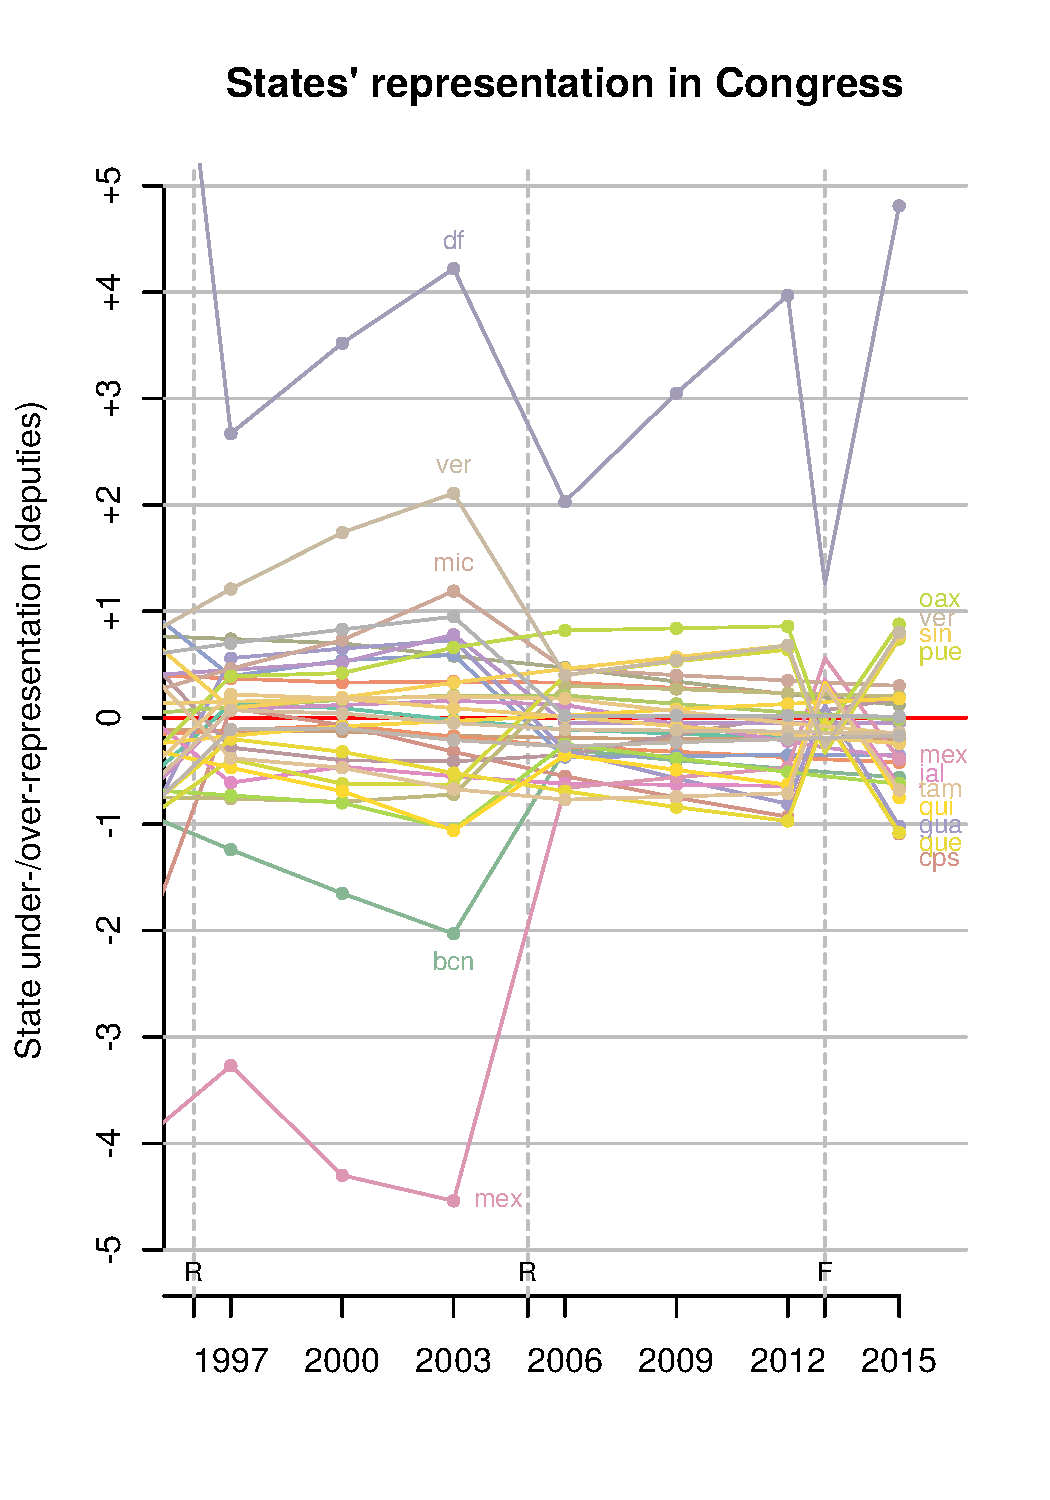
\includegraphics[width=.45\columnwidth]{statesUnderOverRep.pdf} & 
    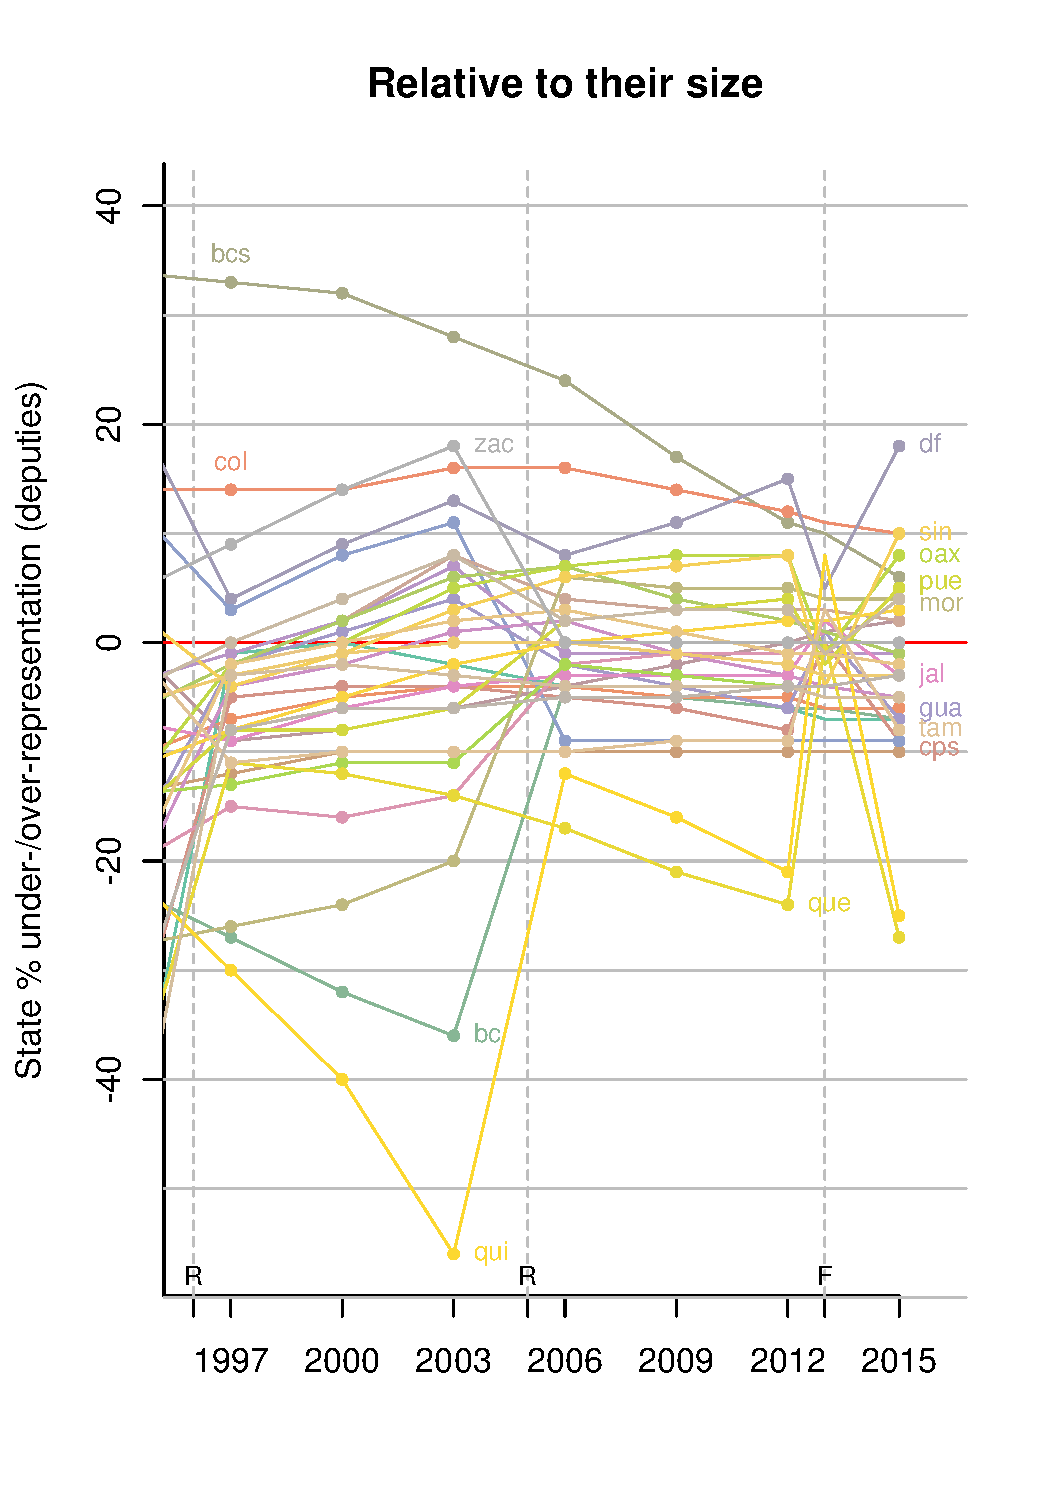
\includegraphics[width=.45\columnwidth]{statesUnderOverRep-rel.pdf} \\ 
  \end{tabular}
  \caption{Demography and state apportionment. Lines connect the lower chamber seats aportioned to seats due difference for each state over time. Letters R in the horizontal axis indicate redistricting, letter F a failed redistricting attempt (reporting the effect it would have had).}\label{F:underOverRep}
\end{center}
\end{figure}

Figure \ref{F:underOverRep} summarizes state's representation in Congress. For each federal election since 1997, we estimate each state's population (with linear interpolation of the 1995, 2000, 2005, and 2010 censi,\footnote{Censi in 1995 and 2005 were partial, those in 2000 and 2010 general.} and linear extrapolation after 2010) to compute its fair share of the 300 congressional seats. The actual number of seats apportioned is subtracted, yielding the state's over- or under-representation. The left panel reports this measure in absolute terms (how many deputies more or less than the state's fair share), the right panel relative to seats apportioned to the state.  

Over- and under-representation vis-\`a-vis demography is one form of malapportionment that few electoral systems can render negligible. Mexico's does not. Since the first term of the measure is an integer but the second a real number, a fraction is bound to remain. Fractions in well-apportioned systems should all be less than 1 in absolute value. The left panel shows that this is mostly the case for Mexico, but exceptions are systematic. It is also plain that redistricting towards 2006 corrected, to some extent, important distortions that redistricting towards 1997 had failed to rectify. Under-representation of Baja California, but especially of the Mexico State dropped respectively from two and five deputies less than due (deficits of 30 percent and less than 10 in relative terms), respectively. Over-represented Veracruz behaved near symmetrically to Baja in absolute terms (not relative). And a distortion strongly favoring the Federal District ($+4$ deputies) was somewhat attenuated towards the 2006 election, but never removed. Relative over-representation is substantial for the smallest states---entitled to two seats at least like all states, which Southern Baja California and Colima weren't really worth demographically until quite recently---migrant-worker-exporter Zacatecas up to 2003, and the Federal District of late. With this brief description, it is puzzling that the redistributive nature of apportionment has not pushed for the adoption of alternative methods. The seventeen states that were under-represented in 2006 jointly controlled a majority (162) of single-member districts; fourteen of them have always been below the red line indicating fair representation. 

Whether distortions are purely mechanical, caused by difficulties to estimate population growth accurately, or purposeful remains an open question. But analysis should be able to detect whether or not this distortion is a source of bias in the translation of votes to seats. 

%Not sure if this is useful anymore... I thought we might discuss what failed redistricting for 2015 would have done. 

% comment [Mike] Bernie Grofman wrote a co-authored paper (I'll have to dig up the cite) that decomposed bias into apportionment, malapportionment, and redistricting effects. Perhaps we take a similar approach in future revisions? If the manuscript goes that direction, the apportionment section should go before redistricting since apportionment occurs before redistricting. 

\begin{tabular}{l|c|c|}
                  & \mc{2}{c}{Would 2013 have reverted?}\\ \cline{2-3}
State is          & yes                  & no \\ \hline
over-represented  & df oax pue sin       & bcs col\\ \hline
under-represented &  cps gua que qui tam & ags bc cam coa dgo\\ \hline
                  &                      & cua gue hgo mic mor  \\ 
on target         & jal mex ver          & nay nl san son tab  \\ 
                  &                      & tla yuc zac \\ \hline
\end{tabular}

\section{One Person, One Vote?}

Despite automation and straightforward, formal redistricting criteria, Mexican parties in general, and IFE in particular, have been remarkably tolerant to unequally sized districts --- another form of malapportionment. It is related in some degree to distortions last discussed because differences in state apportionment perforce create size differences \emph{across} states. But size inequality \emph{within} states is also observed and substantial. 

\begin{figure}
\begin{center}
    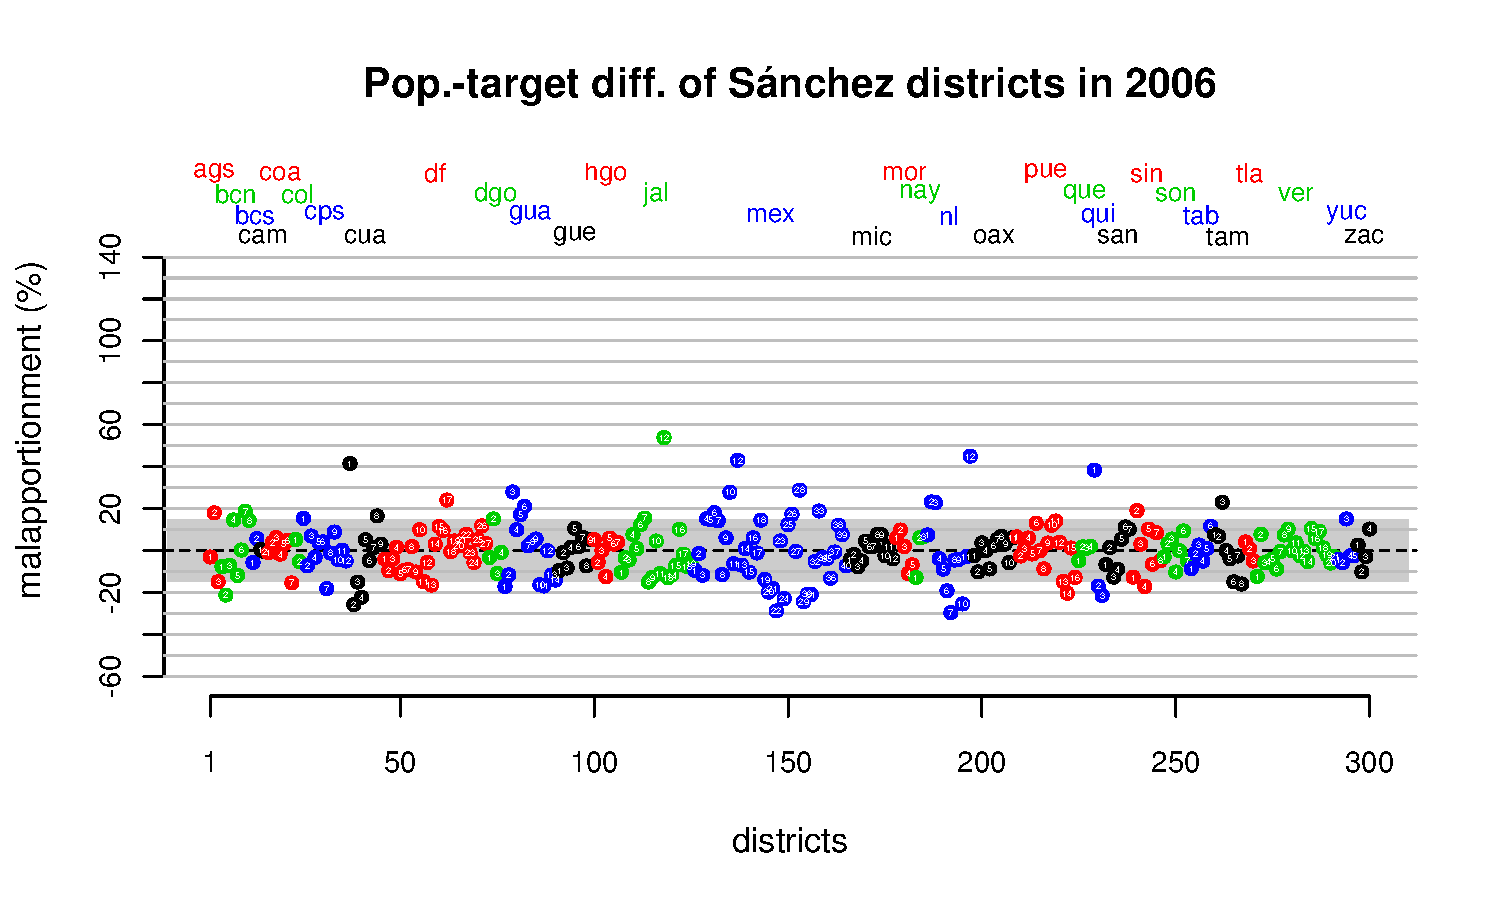
\includegraphics[width=.7\columnwidth]{malapp2006d0.pdf} \\
    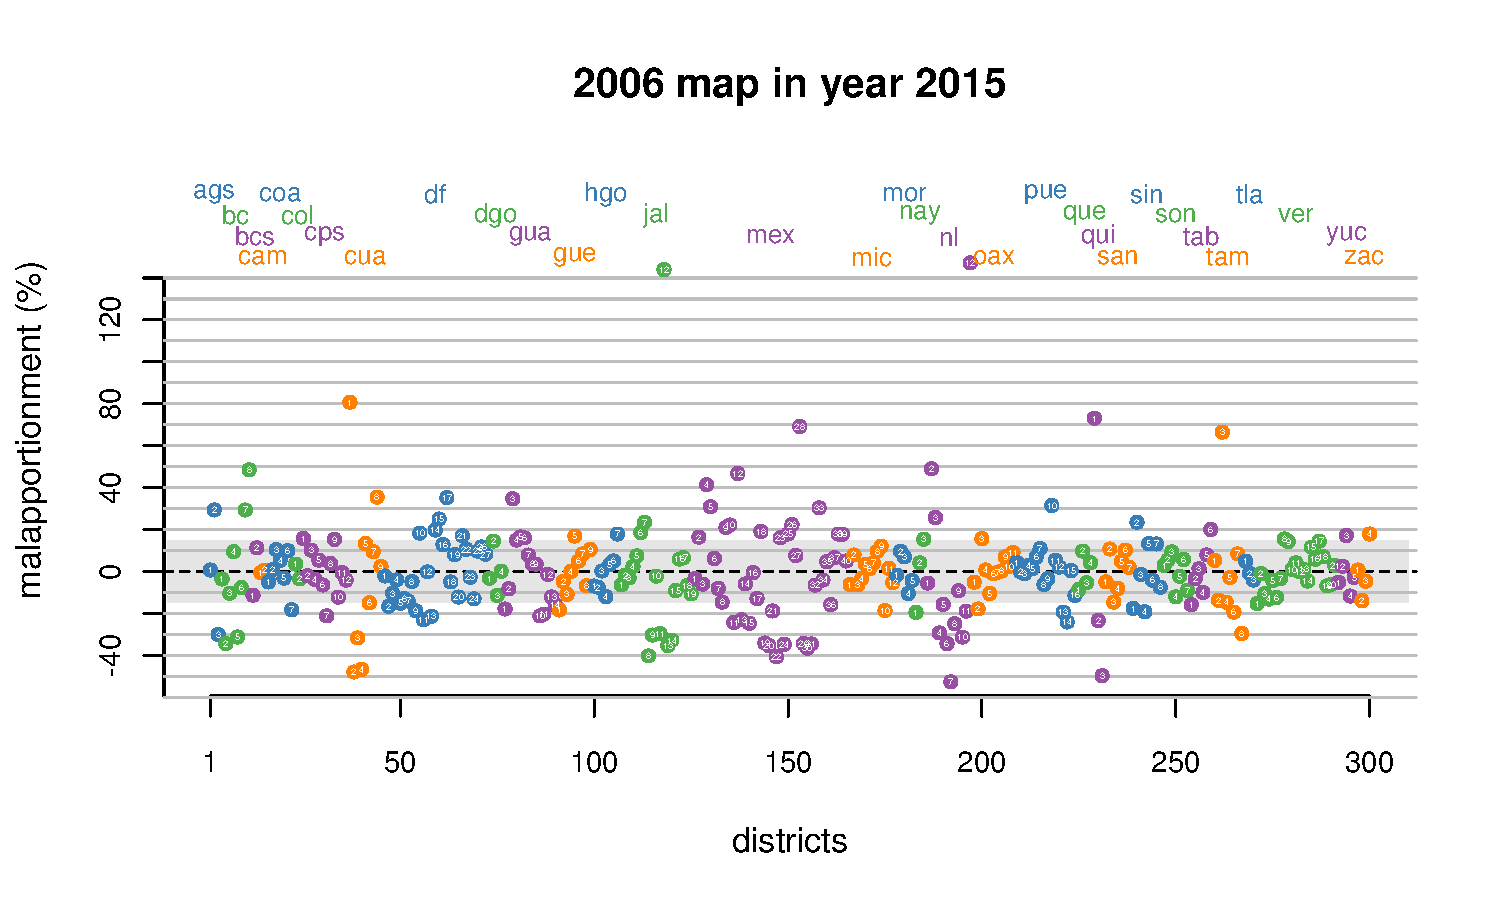
\includegraphics[width=.7\columnwidth]{malapp2015d0.pdf} \\
    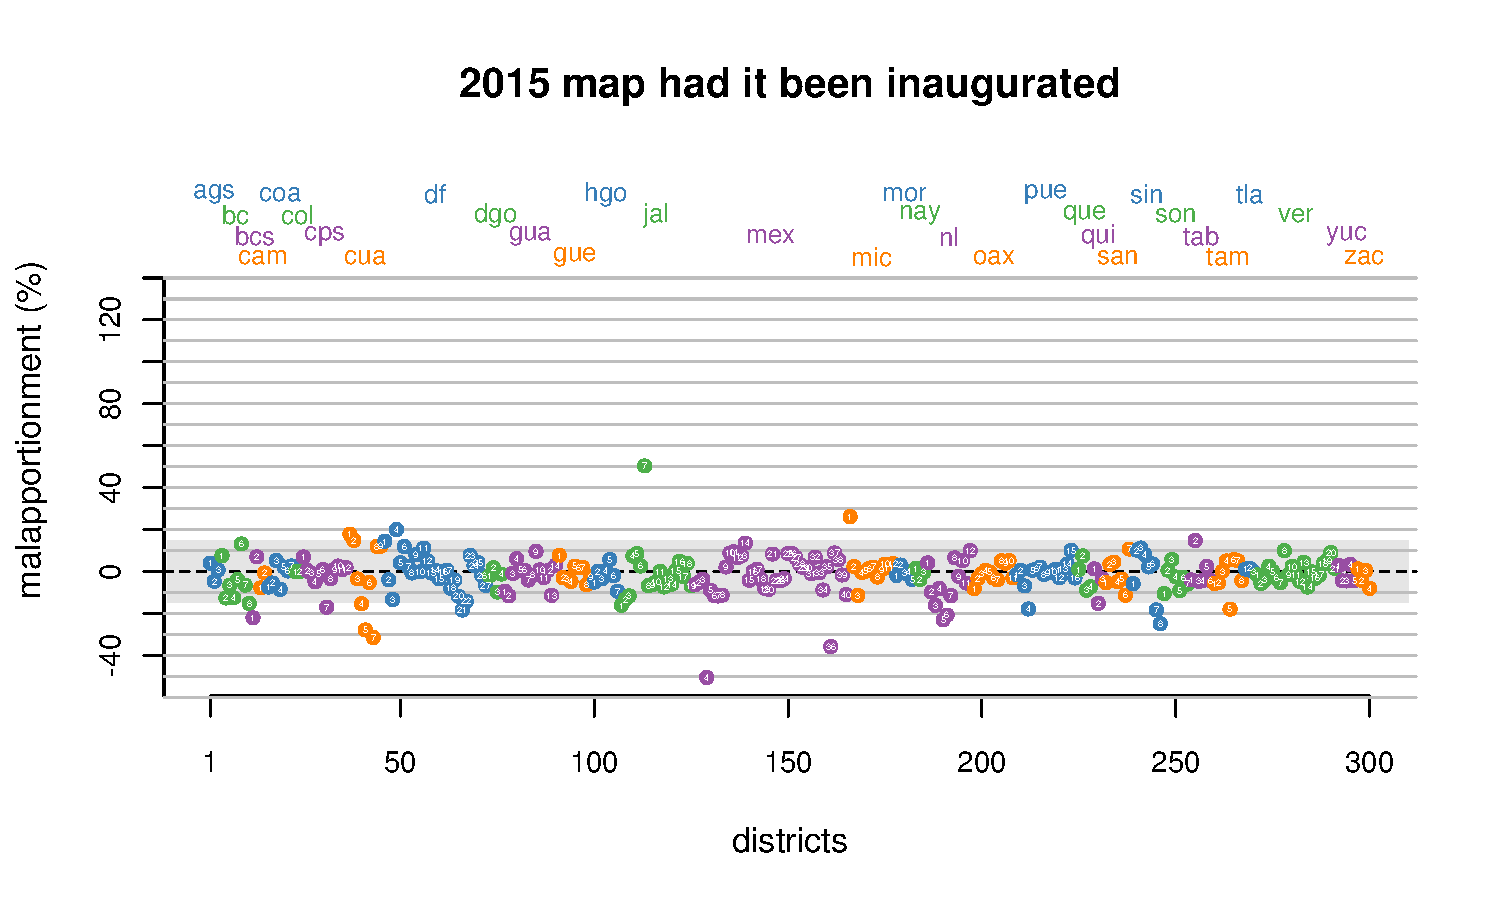
\includegraphics[width=.7\columnwidth]{malapp2015d3.pdf} \\
  \caption{Malapportionment through years and maps. The $y$-scale measures district population relative to ideal (mean state population). The grey band is IFE's range of tolerance for district population asymmetries.}\label{F:malapp}
\end{center}
\end{figure}

Small deviations around a state's mean district population are unavoidable. But what constitutes a small deviation remains a matter of opinion. Courts in the U.S. have struck down district maps bearing less than 1\% differences without proper justification \citep{tuckerApportionment.1985}. Redistricting authorities generally view a \emph{de minimus} population deviations of as little as one or zero persons between congressional districts as desirable to inoculate against litigation. In stark contrast, when redistricting, IFE considered deviations between 10 and 15\% above or below mean state district size perfectly normal. Within such spread, a district at the bottom end is worth one-third more in Congress than one at the top end. Surprisingly, no party has ever challenged this in Court. 

Moreover, Mexico's redistricting automation makes no attempt for districts within states to tend towards zero malapportionment, with only exceptional deviants within the range of tolerance. The preservation of municipal boundaries, for instance, is achieved by exploiting tolerated leeway. Figure \ref{F:malapp} shows how the tolerance band is uniformly occupied by districts even right after inception. It is notable that the new 2006 map had so many districts outside the range of tolerance. 

When redistricting plans are drawn, malapportionment does not legally exist. Mexico's constitution provides that every redistricting process must rely on the most recent population census available, with no attempt to estimate population change since (and, unlike the U.S., no obligation to redistrict as soon as a new census is available). By 2006, population changes from 2000 to 2005 resulted in the mean state population that year deviating 9.7 percent compared to the census, with a standard deviation of 6.9 percent. Variance cannot be smaller when dealing with sub-state units used to prepare districts, pushing about 80 new districts out of the broad $\pm 15$\% band.\footnote{Census data reported at the electoral section level are available since 2005 only. We could repeat this exercise at the municipal level to approximate distortions that the law pushed IFE to introduce better.} The requirement to keep municipalities with large indigenous population within the same district may also explain exceptions. Median absolute district malapportionent of the 2006 map upon inauguration was 6.5\%, the third quartile surpassing the ten point tolerance margin at 12.4\% \citep[also,][]{trelles.mtz.tesisItam.2007}. For next year's midterm election, the same descrepancies will be 9.9 and 17.9\%, respectively. The abandoned 2015 map proposal did a better job upon inauguration, with median absolute district malapportionment of 4.2\% and third quartile at 8.1\%. 

\begin{tabular}{lrrrrr}
                 & \mc{5}{c}{Absolute malapportionment} \\
Map in year      & Min. & 1st quartile & median & 3rd quartile & max. \\ \hline
2006 map in 2006 & $<.01$ & 3.4 & 6.5 & 12.4 & 54.8 \\
2006 map in 2015 & .02 & 4.4 & 9.9 & 18.0 & 147.2 \\
2015 map in 2015 & .01 & 1.9 & 4.2 & 8.1 & 50.6 \\
\end{tabular}

Whether districts below and above fair representation behave differently merits closer inspection. Whether due to technical difficulties or discretion, malapportionment may be the source of meaningful distortions in democratic representation.

\section{The 2006 Map and the 2015 Proposals}

%*** Elements of Alejandro's discussion in the APSA2014Paper of redistricting process could fit well here (file available in the G drive). ***

A new map is a full description of district boundary changes. The common way to visualize a map is by drawing it. We look at maps differently, with focus not in the physical lines and line changes but in their political consequences. Putting the 2006 map and the 2015 final proposal drawings side to side reveals boundary shifts. But unless the drawing is more data rich, assessing even the relatively simple question of how similar districts were before and after redistricting visually is a challenge. 

\begin{table}
\begin{center}
  \begin{tabular}{lrrrrr}
  Similarity between                 &   min  &  25\%  & median &  75\% &  max \\ \hline
  first 2015 proposal and status quo & 0.128  & 0.419  & 0.584  & 0.755 &  1   \\
  final 2015 proposal and status quo & 0.125  & 0.437  & 0.643  & 0.805 &  1   \\
  first and final 2015 proposals     & 0.174  & 0.705  & 0.967  & 1     &  1   \\
  \end{tabular}
  \caption{District similarity before and after the failed 2015 redistricting}\label{T:simIndex}
\end{center}
\end{table}

But a similarity index \citep[][:15--7]{cox.katz.2002} offers ground for assessment. Measurement identifies the parent district or single largest contributor of population to every new district. The $s$imilarity index divides the population that $p$arent and $n$ew district share in $c$ommon by their joint population: $s = c / (p + n - c)$. The range is zero (district shares no population at all with parent) to one (districts are identical). Table \ref{T:simIndex} describes the change that the 2015 map would have brought in the 300 single member districts, comparing IFE's initial and final proposals with the 2006 map. Also compared are the final and initial 2015 proposals themselves. 

Six percent of districts entertained no change in boundaries whatsoever vis-\`a-vis the status quo (18 districts in the initial proposal, 19 in the final), and twice as many had at least nine-tenths of the population in common (40 districts in the initial, 44 in the final proposal). Inspecting which districts were \emph{a priori} chosen for marginal or no change might reveal systematic distortions of the automated redistricting algorithm. Party feedback left 39 percent of districts in IFE's first proposal intact, and 62 percent with up from nine-tenths of the population in common. Inspecting which districts the parties targeted for major amendment --- presumably a partial reinstatement of a preferred status quo district --- should shed further light into the subject. Note how median district similarity with the 2006 map augmented from first to final proposal. So did the third quartile. Accepted counter-proposals therefore reconstituted portions of status quo districts. This seems consistent with a view where parties protect strongholds that the algorithm may have split, but further analysis must be done. 

% comment [Mike] but, the counter-proposals also improved the cost function. What this suggests is that parties will not propose amendments that do not improve their position. A straight-forward proposition, but an important one nonetheless. Still, other parties might propose plans that hurt rivals. The plans PRD plans that improved the score but were not adopted may be a smoking gun since those plans may have disrupted other parties' districts. The 6 percent of districts that had no change may be because population changes within these states are minimal and the optimal plan has already been identified in the 2006 redistricting.

% comment [Eric] Mike points to something potentially interesting for this or another paper. Could we reconstruct the counteroffers that parties made in some districts and cross that with recent electoral history in those districts?

% comment [Alejandro] Yes we could... We have all the information, right?

Noting that victory margins began widening in the mid-1960s, \citet{mayhew1974vanishingMg} saw gerrymandering as one possible explanation, incumbents influencing the preservation of safe districts. While the argument opened the heated incumbency advantage debate, the intuition may guide our inquiry. District volatility should capture a key element for analysis of map similarities. District $d$ volatility is $v_d = 1/2 \sqrt{ \sum_{p=1}^P \sum_{t=2}^3 (v_{d,p,t}- v_{d,p,t-1})^2 }$ with $p$ indexing the competing parties and $t=1,2,3$ for the 2006,  2009, and 2012 congressional elections respectively.\footnote{The measure of volatility proposed is inspired in measures of disproportionality, replacing the seats--votes difference with vote first differences. It is a squared version of a Loosemore-Hanby index \citep{loosemore.hanbyDisproportionality1971,gallagherDisproportionality1991}.} 

Mexican party strength is not proportional to the formidable entry barriers they enjoy and massive public subsidies they receive yearly \citep{magar.2007ref.2015}. Evidence of this is their inability to cultivate loyal voters. District volatility is remarkably high, as shown in Table \ref{T:volatMarginsd0}. The median district saw 25 percent of votes change party hands between 2006 and 2012 (not exactly how the index reads, but close enough). With so many volatile districts around, parties should have attempted to redress strongholds that automated redistricting split beyond recognition. How much were strongholds affected by the initial 2015 proposal? To what extent did party counter-proposals redress them? This should be a promising line of inquiry. 

\begin{table}
\begin{center}
\begin{tabular}{lrrrrr}
                    &  min.   &  25\%   & median  & 75\%   & max \\ \hline
district volatility &  .08    & .19     & .25     & .31    & .52 \\
mean PAN margin     &  $-.49$ & $-.23$  & $-.10$  & .01    & .28 \\   
mean PRI margin     &  $-.43$ & $-.09$  & $-.01$  & .07    & .28 \\   
mean PRD margin     &  $-.51$ & $-.31$  & $-.21$  & $-.04$ & .39 \\
\end{tabular}
\caption{2006 map district volatility and party margins in three congressional elections}\label{T:volatMarginsd0}
\end{center}
\end{table}

% comment [Eric] One possibility is regressing new district similarity on mean 2006--12 parent district margin, low volatility, and their interaction. Another route is the estimation of district elasticities---how vote swings in a district's sections respond to statetwide party swings. This could provide an alternative approach to explain the district similarity index. The appendix has preliminary elasticity estimates and some discussion.

\section{Winners and Losers}

Party effects of redistricting should involve seat swaps, to which this section turns to. Counter-factual analysis looks at how votes would have converted to seats in recent congressional elections had the 2015 map (the third scenario) been used in stead of the status quo. M\'arquez (\href{http://bit.ly/1nk4kYs}{\url{http://bit.ly/1nk4kYs}}) did this using national-level data over two decades. We proceed with state-by-state breakdowns over much a shorter span (2006, 2009, and 2012), uncovering many seat changes that cancel out in the aggregate. Compared to the status quo, counter-factual districts would slightly benefit the PRI nationwide and, by alliance, the Green party, granting them 2 to 3 extra deputies; would slightly hurt the PAN, erasing 2 to 4 victories; and would, on average, leave the left unaffected. Analysis also reveals distributive effects in nearly half the states, which complicates the assessment of partisan effects of the redistricting proposal. Counterfactuals are prepared with IFE's first and final (third) 2015 redistricting proposals, offering perspective to appreciate whether and how parties influence expert electoral regulation in general \citep{estevez.magar.rosas.2008}, and district line drawing in particular \citep{rossiter.etal.1997,cox.katz.2002}. 

% comment [Mike] I am not certain what the counter-factual plans are. Are they the plans drawn by Eric's students? Are they the first and third scenarios for the 2015 redistricting?

% comment [Alejandro]:The counterfactual plan/results were calculated by Eric, not his students.  Using  electoral results from Mexico's 300 SMD in 2006, 2009 and 2012, he build two counterfactual (hypothetical) scenarios: 1) Electoral results using the IFEs 2013 FIRST SCENARIO (pure optimization), and 2) Electoral results using IFEs 2013 THIRD SCENARIO (optimization + party counterporposals). 


Column $S$ of Tables \ref{T:2006}, \ref{T:2009}, and \ref{T:2012} breaks down the federal deputy seats that parties won in the last three congressional elections by state (with actual districts). Columns $\Delta_1$ and $\Delta_3$ report seat changes had map proposals 1 and 3, respectively, been used instead. Changes are computed adding up section-level vote returns into districts. For the sake of readability, the tables do not distinguish seats that the PRI won with the Green party (PVEM) as coalition partner.\footnote{Nine states (two in 2009, seven in 2012) combining districts with joint PRI--Green candidate and districts where each fielded a candidate complicate counterfactual computation. Most counterfactual districts in such states blend sections with and without coalition votes, so a decision about their coalition status has to be made. I looked at whether or not coalition sections are the most numerous in the new district, classifying it accordingly. As a consequence, several seats won in status quo districts swap from the PRI to the coalition and vice versa in mixed states' counterfactuals---mostly in the State of Mexico 2009. Keeping such swaps in the count artificially inflates the redistributive effects of redistricting.} In 2009, PRI and partner competed against each other in 237 districts while fielding joint candidates in the remaining 63, and in 2012 they competed in 101 and shared candidate in 199. Coalition in 2006 was nationwide, like that of the PRD and two minor left parties in 2006 and 2009, removing complications. 

% pri coalition info:
% 2009
% 237 districts in 29 states with no coalition 
% 63 districts in 11 states with PRI-PVEM coalition
%  of which 46 districts in 9 states with mixed coalition status
% 2012
% 101 districts in 19 states with no coalition
% 199 districts in 13 srtates with PRI-PVEM coalition
%  of which XX in 7 states with mixed coalition status

\begin{table}
\begin{center}
 \begin{tabular}{rrrr|rrr|rrr}
      & \multicolumn{3}{c}{PAN} & \multicolumn{3}{c}{PRI coalition} & \multicolumn{3}{c}{PRD coalition} \\
state &$S$& $\Delta_1$ &  $\Delta_3$ & $S$& $\Delta_1$ &  $\Delta_3$ & $S$& $\Delta_1$ &  $\Delta_3$  \\ \hline
ags &   3 &     &     &      &      &      &      &      &        \\       
 bc &   8 &     &     &      &      &      &      &      &        \\       
bcs &     &     &     &      &      &      &    2 &      &        \\       
cam &     &     &     &    2 &      &      &      &      &        \\       \hdashline
coa &   5 & $-1$& $-1$&    2 &  $+1$&  $+1$&      &      &        \\       
col &   2 &     &     &      &      &      &      &      &        \\       
cps &     &     & $+1$&    7 &  $-1$&      &    5 &  $+2$&        \\       
cua &   4 & $+2$&     &    5 &  $-2$&      &      &      &        \\       \hdashline
 df &   2 &     &     &      &      &      &   25 &  $-3$&  $-3$  \\       
dgo &   1 & $+1$& $+1$&    3 &  $-1$&  $-1$&      &      &        \\       
gua &  14 & $+1$& $+1$&      &      &      &      &      &        \\       
gue &     &     &     &      &      &      &    9 &      &        \\       \hdashline
hgo &   1 &     &     &    4 &      &  $-1$&    2 &      &  $+1$  \\       
jal &  18 & $+1$& $+1$&    1 &      &      &      &      &        \\       
mex &  11 & $-1$&     &    6 &  $+1$&  $-1$&   23 &  $+1$&  $+2$  \\       
mic &   4 &     &     &      &      &      &    8 &      &        \\       \hdashline
mor &   2 &     & $-1$&    1 &  $-1$&      &    2 &  $+1$&  $+1$  \\       
nay &     &     &     &    2 &      &      &    1 &      &        \\       
 nl &   7 & $-1$& $-1$&    5 &  $+1$&  $+1$&      &      &        \\       
oax &     &     &     &    2 &      &      &    9 &  $-1$&  $-1$  \\       \hdashline
pue &  11 & $-1$& $-1$&    5 &  $-1$&      &      &  $+1$&        \\       
que &   4 & $+1$& $+1$&      &      &      &      &      &        \\       
qui &     &     &     &    2 &      &      &    1 &  $+1$&  $+1$  \\       
san &   7 &     &     &      &      &      &      &      &        \\       \hdashline
sin &   2 &     &     &    6 &  $-1$&  $-1$&      &      &        \\       
son &   5 &     &     &    2 &      &      &      &      &        \\       
tab &     &     &     &      &      &      &    6 &      &        \\       
tam &   5 & $+1$& $+1$&    3 &      &      &      &      &        \\       \hdashline
tla &   2 &     &     &      &      &      &    1 &      &        \\       
ver &  11 & $-3$& $-5$&    6 &  $+2$&  $+4$&    4 &      &        \\       
yuc &   4 & $-1$& $-1$&    1 &  $+1$&  $+1$&      &      &        \\       
zac &   1 &     &     &      &      &      &    3 &      &        \\ \hline 
tot & 134 & $-1$& $-4$&   65 &  $-1$&  $+3$&  101 &  $+2$&  $+1$  \\       
abs &     & $15$& $16$&      &  $13$&  $11$&      &  $10$&  $9$  \\       
\end{tabular}
\caption{Seats won by state and counterfactual differences in 2006. Columns $\Delta_1$ and $\Delta_3$ report change in $S$eats won with proposals 1 and 3 (discussed in text), respectively. Row tot reports column sum, row abs the sum of absolute column values.}\label{T:2006}
\end{center}
\end{table}


\begin{table}
\begin{center}
\begin{tabular}{rrrr|rrr|rrr|rrr}
      & \multicolumn{3}{c}{PAN} & \multicolumn{3}{c}{PRI$^*$} & \multicolumn{3}{c}{PRD} & \multicolumn{3}{c}{Other} \\
state &$S$& $\Delta_1$ &  $\Delta_3$ & $S$& $\Delta_1$ &  $\Delta_3$ & $S$& $\Delta_1$ &  $\Delta_3$ & $S$& $\Delta_1$ &  $\Delta_3$ \\ \hline
ags &   2 &     &     &   1 &     &     &     &     &      &    &    & \\       
 bc &   8 &     &     &     &     &     &     &     &      &    &    & \\       
bcs &     &     &     &     &     &     &   2 &     &      &    &    & \\       
cam &     &     &     &   2 &     &     &     &     &      &    &    & \\       \hdashline
coa &     &     &     &   7 &     &     &     &     &      &    &    & \\       
col &   1 &     &     &   1 &     &     &     &     &      &    &    & \\       
cps &   4 & $+1$& $-1$&   4 &     & $+3$&   4 &     & $-1$ &    &    & \\       
cua &   1 & $-1$& $-1$&   8 & $+1$& $+1$&     &     &      &    &    & \\       \hdashline
 df &   6 & $-1$& $-1$&   1 &     &     &  17 & $-2$& $-2$ & 3  &    & \\       
dgo &     &     &     &   4 &     &     &     &     &      &    &    & \\       
gua &  13 & $+1$& $+1$&   1 &     &     &     &     &      &    &    & \\       
gue &     &     &     &   8 &     &     &   1 &     &      &    &    & \\       \hdashline
hgo &     &     &     &   7 &     &     &     &     &      &    &    & \\       
jal &   9 & $+2$& $+3$&  10 & $-1$& $-2$&     &     &      &    &    & \\       
%mex &   2 &     &     &   8 & $-3$& $-2$&     &     &      &    &    & \\       
mex &   2 &     &     &  38 & $+1$& $+1$&     &     &      &    &    & \\       
mic &   4 & $+1$&     &     &     &     &   8 & $-1$&      &    &    & \\      \hdashline 
mor &     &     &     &   5 &     &     &     &     &      &    &    & \\       
nay &   1 &     &     &   1 &     &     &   1 &     &      &    &    & \\       
 nl &   5 & $-1$& $-1$&   7 & $+1$& $+1$&     &     &      &    &    & \\       
oax &     &     &     &  11 & $-1$& $-1$&     &     &      &    &    & \\       \hdashline
pue &     & $+2$& $+1$&  16 & $-3$& $-2$&     &     &      &    &    & \\       
que &   1 & $+1$&     &   3 &     & $+1$&     &     &      &    &    & \\       
qui &     &     &     &   3 & $+1$& $+1$&     &     &      &    &    & \\       
san &   5 &     &     &   2 &     &     &     &     &      &    &    & \\       \hdashline
sin &     & $+1$& $+1$&   8 & $-2$& $-2$&     &     &      &    &    & \\       
son &   2 &     &     &   5 &     &     &     &     &      &    &    & \\       
tab &     &     &     &   4 &     &     &   2 &     &      &    &    & \\       
tam &     &     &     &   8 & $+1$& $+1$&     &     &      &    &    & \\       \hdashline
tla &   3 &     &     &     &     &     &     &     &      &    &    & \\       
ver &   4 & $-2$& $-2$&  17 & $+1$& $+1$&     &     &      &    &    & \\       
yuc &     &     &     &   5 &     &     &     &     &      &    &    & \\       
zac &     &     &     &     &     &     &   4 &     &      &    &    & \\ \hline 
%tot &  71 & $+4$&     & 137 & $-6$& $-4$&  39 & $-3$& $-3$ & 3  &    & \\       
tot &  71 & $+4$&     & 187 & $-1$& $+3$&  39 & $-3$& $-3$ & 3  &    & \\       
abs &     & $14$& $12$&      &$13$& $17$&      & $3$&  $3$ &    &    & \\       
% \begin{tabular}{rrrr|rrr|rrr|rrr|rrr}
%       & \multicolumn{3}{c}{PAN} & \multicolumn{3}{c}{PRI} & \multicolumn{3}{c}{PRI coalition} & \multicolumn{3}{c}{PRD} & \multicolumn{3}{c}{Other} \\
% state &$S$& $\Delta_1$ &  $\Delta_3$ & $S$& $\Delta_1$ &  $\Delta_3$ & $S$& $\Delta_1$ &  $\Delta_3$ & $S$& $\Delta_1$ &  $\Delta_3$ & $S$& $\Delta_1$ &  $\Delta_3$ \\ \hline
% ags &   2 &     &     &   1 &     &     &      &      &      &     &     &      &    &    & \\       
%  bc &   8 &     &     &     &     &     &      &      &      &     &     &      &    &    & \\       
% bcs &     &     &     &     &     &     &      &      &      &   2 &     &      &    &    & \\       
% cam &     &     &     &   2 &     &     &      &      &      &     &     &      &    &    & \\       \hdashline
% coa &     &     &     &   7 &     &     &      &      &      &     &     &      &    &    & \\       
% col &   1 &     &     &   1 &     &     &      &      &      &     &     &      &    &    & \\       
% cps &   4 & $+1$& $-1$&     &     &     &    4 &      &  $+3$&   4 &     & $-1$ &    &    & \\       
% cua &   1 & $-1$& $-1$&   8 & $+1$& $+1$&      &      &      &     &     &      &    &    & \\       \hdashline
%  df &   6 & $-1$& $-1$&     &     &     &    1 &      &      &  17 & $-2$& $-2$ & 3  &    & \\       
% dgo &     &     &     &   4 &     &     &      &      &      &     &     &      &    &    & \\       
% gua &  13 & $+1$& $+1$&     &     &     &    1 &      &      &     &     &      &    &    & \\       
% gue &     &     &     &   6 &     &     &    2 &      &      &   1 &     &      &    &    & \\       \hdashline
% hgo &     &     &     &   6 &     &     &    1 &      &      &     &     &      &    &    & \\       
% jal &   9 & $+2$& $+3$&   7 & $-1$& $-2$&    3 &      &      &     &     &      &    &    & \\       
% %mex &   2 &     &     &   8 & $-3$& $-2$&   30 &  $+4$&  $+3$&     &     &      &    &    & \\       
% mex &   2 &     &     &     &     &     &$38^*$&  $+1$&  $+1$&     &     &      &    &    & \\       
% mic &   4 & $+1$&     &     &     &     &      &      &      &   8 & $-1$&      &    &    & \\      \hdashline 
% mor &     &     &     &   5 &     &     &      &      &      &     &     &      &    &    & \\       
% nay &   1 &     &     &   1 &     &     &      &      &      &   1 &     &      &    &    & \\       
%  nl &   5 & $-1$& $-1$&   7 & $+1$& $+1$&      &      &      &     &     &      &    &    & \\       
% oax &     &     &     &  11 & $-1$& $-1$&      &      &      &     &     &      &    &    & \\       \hdashline
% pue &     & $+2$& $+1$&  15 & $-3$& $-2$&    1 &      &      &     &     &      &    &    & \\       
% que &   1 & $+1$&     &   3 &     & $+1$&      &      &      &     &     &      &    &    & \\       
% qui &     &     &     &   1 &     &     &    2 &  $+1$&  $+1$&     &     &      &    &    & \\       
% san &   5 &     &     &   2 &     &     &      &      &      &     &     &      &    &    & \\       \hdashline
% sin &     & $+1$& $+1$&   8 & $-2$& $-2$&      &      &      &     &     &      &    &    & \\       
% son &   2 &     &     &   5 &     &     &      &      &      &     &     &      &    &    & \\       
% tab &     &     &     &   4 &     &     &      &      &      &   2 &     &      &    &    & \\       
% tam &     &     &     &   8 & $+1$& $+1$&      &      &      &     &     &      &    &    & \\       \hdashline
% tla &   3 &     &     &     &     &     &      &      &      &     &     &      &    &    & \\       
% ver &   4 & $-2$& $-2$&  17 & $+1$& $+1$&      &      &      &     &     &      &    &    & \\       
% yuc &     &     &     &     &     &     &    5 &      &      &     &     &      &    &    & \\       
% zac &     &     &     &     &     &     &      &      &      &   4 &     &      &    &    & \\ \hline 
% %tot &  71 & $+4$&     & 137 & $-6$& $-4$&   50 &  $+5$&  $+7$&  39 & $-3$& $-3$ & 3  &    & \\       
% tot &  71 & $+4$&     & 129 & $-3$& $-2$&$58^*$&  $+2$&  $+5$&  39 & $-3$& $-3$ & 3  &    & \\       
\end{tabular}
\caption{Seats won by state and counterfactual differences in 2009. See Table \ref{T:2006} for column and row label meanings. $^*$Includes 50 seats that the PRI won in coalition in 63 districts from 10 states.}\label{T:2009}
% \caption{Seats won by state and counterfactual differences in 2009. See Table \ref{T:2006} for column label meanings. $^*$Includes 8 seats the PRI won solo, see text for details.}\label{T:2009} 
\end{center}
\end{table}


\begin{table}
\begin{center}
\begin{tabular}{rrrr|rrr|rrr|rrr}
      & \multicolumn{3}{c}{PAN} & \multicolumn{3}{c}{PRI$^*$} & \multicolumn{3}{c}{PRD coalition} & \multicolumn{3}{c}{Other} \\
state &$S$& $\Delta_1$ &  $\Delta_3$ & $S$& $\Delta_1$ &  $\Delta_3$ & $S$& $\Delta_1$ &  $\Delta_3$ & $S$& $\Delta_1$ &  $\Delta_3$ \\ \hline
ags &   2 & $-1$& $-1$&   1 & $+1$& $+1$&      &      &       &    &    & \\       
 bc &   1 &     &     &   7 &     &     &      &      &       &    &    & \\       
bcs &   2 &     &     &     &     &     &      &      &       &    &    & \\       
cam &     &     &     &   2 &     &     &      &      &       &    &    & \\       \hdashline
coa &   3 &     &     &   4 &     &     &      &      &       &    &    & \\       
col &     &     &     &   2 &     &     &      &      &       &    &    & \\       
cps &     &     &     &   9 & $+1$& $+2$&      &      &       & 3  &    & $-1$ \\       
cua &   1 & $-1$&     &   8 & $+1$&     &      &      &       &    &    & \\       \hdashline
 df &   1 &     &     &     &     &     &   26 &  $-3$&  $-3$ &    &    & \\       
dgo &     &     &     &   4 &     &     &      &      &       &    &    & \\       
gua &   7 & $+2$& $+2$&   7 & $-1$& $-1$&      &      &       &    &    & \\       
gue &     &     &     &     &     &     &    9 &      &       &    &    & \\       \hdashline
hgo &     &     &     &   7 &     &     &      &      &       &    &    & \\       
jal &   1 &     &     &  18 &     &     &      &  $+1$&  $+1$ &    &    & \\       
mex &   1 & $-1$& $-1$&  31 & $+3$& $+2$&    8 &  $-1$&       &    &    & \\       
mic &     &     &     &   8 & $+1$&     &    4 &  $-1$&       &    &    & \\       \hdashline
mor &     &     &     &   1 &     &     &    4 &      &       &    &    & \\       
nay &     &     &     &   3 &     &     &      &      &       &    &    & \\       
 nl &   6 & $-2$& $-2$&   6 & $+2$& $+2$&      &      &       &    &    & \\       
oax &     &     &     &   1 & $-1$& $-1$&   10 &      &       &    &    & \\       \hdashline
pue &   4 & $-1$&     &  12 & $-1$& $-2$&      &  $+1$&  $+1$ &    &    & \\       
que &   2 & $+1$& $+1$&   2 &     &     &      &      &       &    &    & \\       
qui &     &     &     &   2 &     &     &    1 &  $+1$&  $+1$ &    &    & \\       
san &   2 & $+1$&     &   5 & $-1$&     &      &      &       &    &    & \\       \hdashline
sin &   2 &     &     &   6 & $-1$& $-1$&      &      &       &    &    & \\       
son &   5 &     &     &   2 &     &     &      &      &       &    &    & \\       
tab &     &     &     &     &     &     &    6 &      &       &    &    & \\       
tam &   6 & $-1$& $-1$&   2 & $+2$& $+2$&      &      &       &    &    & \\       \hdashline
tla &     &     &     &   1 &     &     &    2 &      &       &    &    & \\       
ver &   5 & $+1$&     &  15 & $-2$& $-1$&    1 &      &       &    &    & \\       
yuc &   1 &     &     &   4 &     &     &      &      &       &    &    & \\       
zac &     &     &     &   4 &     &     &      &      &       &    &    & \\ \hline
tot &  52 & $-2$& $-2$& 174 & $+4$& $+3$&   71 &  $-2$&       & 3  &    & $-1$ \\       
abs &     & $12$& $8$ &      &$18$& $15$&      &  $8$ &  $6$  &    &    & $2$  \\       
% \begin{tabular}{rrrr|rrr|rrr|rrr|rrr}
%       & \multicolumn{3}{c}{PAN} & \multicolumn{3}{c}{PRI} & \multicolumn{3}{c}{PRI coalition} & \multicolumn{3}{c}{PRD coalition} & \multicolumn{3}{c}{Other} \\
% state &$S$& $\Delta_1$ &  $\Delta_3$ & $S$& $\Delta_1$ &  $\Delta_3$ & $S$& $\Delta_1$ &  $\Delta_3$ & $S$& $\Delta_1$ &  $\Delta_3$ & $S$& $\Delta_1$ &  $\Delta_3$ \\ \hline
% ags &   2 & $-1$& $-1$&   1 & $+1$& $+1$&      &      &      &      &      &       &    &    & \\       
%  bc &   1 &     &     &     &     &     &    7 &      &      &      &      &       &    &    & \\       
% bcs &   2 &     &     &     &     &     &      &      &      &      &      &       &    &    & \\       
% cam &     &     &     &   1 &     &     &    1 &      &      &      &      &       &    &    & \\       \hdashline
% coa &   3 &     &     &   4 &     &     &      &      &      &      &      &       &    &    & \\       
% col &     &     &     &     &     &     &    2 &      &      &      &      &       &    &    & \\       
% cps &     &     &     &     &     & $+1$&    9 &  $+1$&  $+1$&      &      &       & 3  &    & $-1$ \\       
% cua &   1 & $-1$&     &   8 & $+1$&     &      &      &      &      &      &       &    &    & \\       \hdashline
%  df &   1 &     &     &     &     &     &      &      &      &   26 &  $-3$&  $-3$ &    &    & \\       
% dgo &     &     &     &   4 &     &     &      &      &      &      &      &       &    &    & \\       
% gua &   7 & $+2$& $+2$&     &     &     &    7 &  $-1$&  $-1$&      &      &       &    &    & \\       
% gue &     &     &     &     &     &     &      &      &      &    9 &      &       &    &    & \\       \hdashline
% hgo &     &     &     &   7 &     &     &      &      &      &      &      &       &    &    & \\       
% jal &   1 &     &     &     &     &     &   18 &      &      &      &  $+1$&  $+1$ &    &    & \\       
% mex &   1 & $-1$& $-1$&     &     &     &   31 &  $+3$&  $+2$&    8 &  $-1$&       &    &    & \\       
% mic &     &     &     &   6 & $+1$&     &    2 &      &      &    4 &  $-1$&       &    &    & \\       \hdashline
% mor &     &     &     &     &     &     &    1 &      &      &    4 &      &       &    &    & \\       
% nay &     &     &     &   3 &     &     &      &      &      &      &      &       &    &    & \\       
%  nl &   6 & $-2$& $-2$&     &     &     &    6 &  $+2$&  $+2$&      &      &       &    &    & \\       
% oax &     &     &     &   1 & $-1$& $-1$&      &      &      &   10 &      &       &    &    & \\       \hdashline
% pue &   4 & $-1$&     &   1 &     &     &   11 &  $-1$&  $-2$&      &  $+1$&  $+1$ &    &    & \\       
% que &   2 & $+1$& $+1$&   1 &     &     &    1 &      &      &      &      &       &    &    & \\       
% qui &     &     &     &     &     &     &    2 &      &      &    1 &  $+1$&  $+1$ &    &    & \\       
% san &   2 & $+1$&     &   4 &     &     &    1 &  $-1$&      &      &      &       &    &    & \\       \hdashline
% sin &   2 &     &     &   6 & $-1$& $-1$&      &      &      &      &      &       &    &    & \\       
% son &   5 &     &     &   2 &     &     &      &      &      &      &      &       &    &    & \\       
% tab &     &     &     &     &     &     &      &      &      &    6 &      &       &    &    & \\       
% tam &   6 & $-1$& $-1$&   2 & $+2$& $+2$&      &      &      &      &      &       &    &    & \\       \hdashline
% tla &     &     &     &   1 &     &     &      &      &      &    2 &      &       &    &    & \\       
% ver &   5 & $+1$&     &     &     &     &   15 &  $-2$&  $-1$&    1 &      &       &    &    & \\       
% yuc &   1 &     &     &     &     &     &    4 &      &      &      &      &       &    &    & \\       
% zac &     &     &     &     &     &     &    4 &      &      &      &      &       &    &    & \\ \hline
% tot &  52 & $-2$& $-2$&  52 & $+3$& $+2$&  122 &  $+1$&  $+1$&   71 &  $-2$&       & 3  &    & $-1$ \\       
\end{tabular}
\caption{Seats won by state and counterfactual differences in 2012. See Table \ref{T:2006} for column and row label meanings. $^*$Includes 122 seats that the PRI won in coalition in 199 districts from 17 states.}\label{T:2012}
\end{center}
\end{table}

Seen from the national level (bottom line in each table), distributive effects are quite small. The largest drop observed is 4 seats subtracted from PAN in 2006 by the third proposal ($\Delta_3$), the largest hikes 4 extra seats for PAN in 2006 and PRI in 2009 by the first proposal ($\Delta_1$). Mean changes in the period are milder: proposal 1 returns $+\frac{1}{3}$ seat for PAN on average, $+\frac{2}{3}$ for PRI, and $-1$ for PRD; proposal 3 returns $-2$ for PAN, $+3$ for PRI, and $-\frac{2}{3}$ for the left. Adjustments made from first to final proposal are interesting. Party feedback turned the PRI from loser of one seat to winner of three in both 2006 and 2009, a net change of $\bar{\Delta_3} - \bar{\Delta_1} = 4$. Party feedback hurt the PAN almost symmetrically those years, with net changes between $-3$ and $-4$. The puzzle is that PAN had the most counter-proposals accepted (see Table \ref{T:counterprops}), which could be explained by a priority to preserve margins in strongholds and not just victories. Our analysis could presumably show this. 

Changes nationally do not reach one percent of the full chamber. Yet putting them in contrast with recent events in the electoral arena somewhat increases their relevance. Three deputies more is one-third what the PRI--Green coalition lacks to achieve majority status in the 62nd Legislature (2012--15). And it would have sufficed to win three seats from the PRI in 2000 for the PAN to enjoy the plurality in the chamber in the 58th Legislature (2000--03). In a world of volatile voters and tight margins, characteristic of present-day Mexico, a small difference can have larger consequences. 

National aggregates hide substantive redistricting effects at the state level. In 2006, the year most sensible to redistricting, seat distributions change in 18 states (of 32) with the proposals, but positives and negatives tend to cancel out in the national sum. The sum of absolute state changes ---the bottom row of each table--- reveals how many seat swaps (both for and against) a party experiences with redistricting. That year, the PAN, PRI and PRD would have had 16, 11, and 9 such swaps with the third redistricting proposal, respectively. These figures are between 4 and 9 times larger than national changes. In fact, the PAN's 2009 and PRD's 2012 zero nationwide changes are the sum of, respectively, 12 and 6 statewide absolute swaps that fully cancel one another. Some states by themselves involve larger distributive effects than the party's national total, as was the case of 2009 in Veracruz (PAN would get 5 seats less, PRI 4 more) and Jalisco (PAN would get 3 more seats). 

Eleven seats would swap state party hands in 2006 with the adoption of the third proposal, four in the state of Veracruz only. This count excludes seat changes due to reapportionment---seats that one state party wins or loses with no impact on another's seats\footnote{Based on the last decade's population shifts, seven states are bound to get an extra federal seat (Chiapas, Guanajuato, Jalisco, M\'exico, Qur\'etaro, Quintana Roo, and Tamaulipas), four to lose one (Oaxaca, Puebla, Sinaloa, Veracruz) and the Federal District to lose 3.}---yet is nearly three times larger than national swaps. The ratio of state party seat swaps to national party seat swaps in 2009 and 2012 (ten and eight, respectively) remains about 3. 

All said, inspection of counter-factuals through the lens of recent electoral history suggests that the adoption of the redistricting proposal would have helped the PRI. That party managed to redress district lines in the party ---IFE negotiations to avoid likely seat losses and get likely bonus seats instead. The regulator's decision to celebrate the 2015 midterm congressional election with outdated districts appears to postpone pain for the PAN and the left one election cycle. 


\section{Party Bias and Responsiveness}

This section estimates district responsivity and party bias---two effects of scholarly interest, discussed below. M\'arquez (\href{http://bit.ly/1jgsQXE}{\url{http://bit.ly/1jgsQXE}}) has also approached this with national aggregates, uncovering a degree of responsivity characteristic of Westminster systems and party bias against the PAN under the status quo. By proceeding with state aggregates, much higher responsivity (owing to fewer districts, 9 by state on average) is uncovered, but no apparent party bias in neither the 2006 map nor 2015 proposals. 

\subsection{Systematic Bias}

\begin{figure}
\begin{center}
    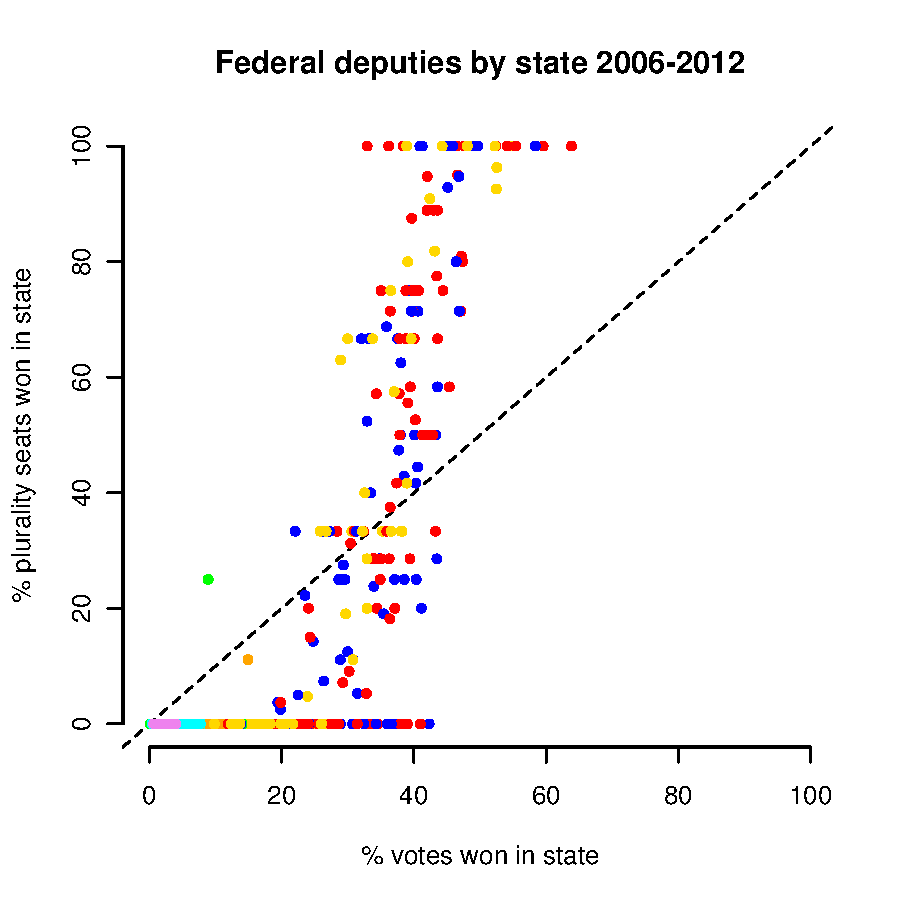
\includegraphics[width=.6\columnwidth]{resXedo20062012.pdf} 
\caption{Seats and votes in the states. Each point is a party-state-year, blue for PAN, red for PRI, gold for PRD, other colors for minor parties.}\label{F:seatsVotes}
\end{center}
\end{figure}

Consider now the relation between party votes and seats portrayed in Figure \ref{F:seatsVotes}. As before, the plot considers plurality seats only and state aggregates. Each point reports the vote share that a party won in a state's federal deputy elections (x-axis) and the share of the state's congressional seats it received (y-axis). Colors distinguish the parties: PAN is blue, PRI is red, PRD is gold, Green is green, among others. For instance, the green dot floating to the left of the cloud is the Green party in Chiapas 2012, where it won 3 of 12 districts. The chart shows that 9 percent of the state's vote awarded the party 25 percent of the seats, an outstanding achievement for any party. The cloud manifests a steep upwards slope characteristic of first-past-the.post systems \citep{taagepera.CubeLaw.1973}.\footnote{Adding the excluded PR seats would level the slope considerably. Doing this would be easy with national aggregates. It is not evident how to carry it with state aggregates, since PR seats are awarded in five second-tier districts joining together several states each.} Points below the diagonal indicate under-representation, those above over-representation. There are notable differences among major parties: the PRI achieved over-representation in three-fifths of election-states between 2006 and 2012, the PAN in two-fifths, and the PRD in one-fourth only. 

With such setting, the possibility that districts are granting undue advantage to the PRI merits closer inspection. A priori, reasons to suspect IFE of cooking districts to favor one party or another are lacking. Major parties, after all, permanently influence the election regulator, ambition counteracting ambition \citep{estevez.magar.rosas.2008}. But that those who draw the district lines can distort a fundamental link of the democratic process is well established in the literature \citep{altman.mcdonald2011bard,cox.katz.2002,engstrom2006redisttrictApsr,rossiter.etal.1997,king.1990elRespBiasMultiparty,balinskiYoung2001FairRep,otero.2003}. Has the insidious gerrymandering reared its ugly head in Mexico? This section estimates majority and party effects in the proposed districts and the status quo. Majority effects are huge, partisan effects negligible. 

\subsection{Two Classes of Distortion}

Undue advantage is known, in the specialized literature, as partisan bias, and is one goal that strategic redistricters pursue. It is not, however, alone: scholarship highlights district responsiveness, also know as majoritarian bias, as another goal. These ought to be distinguished \citep[this paragraph draws heavily on][, ch.\ 3]{cox.katz.2002}. Partisan bias helps the beneficiary buy seats with fewer votes than others. Because seat distribution is a constant sum game, bias in favor of someone always implies bias against someone else. One way of introducing party bias in district lines is with the conventional redistricting strategy known as packing: group your adversary's voters in few districts, wasting votes to win unnecessarily safe seats, raising the price of victory. Responsiveness, on the other hand, is the feature granting a seat bonus to large parties. Maximal responsiveness occurs within each single-member district in isolation: the winner takes all, the rest nothing. The same could be achieved in a whole state by drawing lines so that every district is representative of the state's electorate (Cox and Katz's microcosm strategy). The party with most votes wins every seat, maximizing the vote responsiveness of the proposal. 

Formalizing party bias and responsiveness opens the way towards estimation of these district characteristics. The two-party case is simpler and extends to multiparty systems \citep{taagepera.CubeLaw.1973,tufte1973seatsVotes,king.browning1987biasRespUS}. It is a generalization of the cube law stipulating that 

\begin{equation}
 \frac{s}{1-s} = e^\lambda *  \left(\frac{v}{1-v}\right)^\rho \iff
 \texttt{logit}(s) = \lambda + \rho *  \texttt{logit}(v)
\end{equation}\label{E:cubeLaw}

\noindent where $s$ is the seat share that party 1 won with vote share $v$; $\lambda$ is party 1's bias relative to party 2 (positive values favor party 1, negative values favor party 2); and $\rho$ is the districts' responsiveness. With $\lambda=0$ a system with no party bias ensues. Figure \ref{F:lambdaRhoEx} shows how the parameters affect the vote-to-seats conversion. 

% comment [Mike] how do multiple parties affect bias/responsiveness estimates, compared to two-party setting? I would expect that a party would often need less than 50% of the vote to win 50% of seats due to many parties receiving votes in single-member districts.

\begin{figure}
\begin{center}
    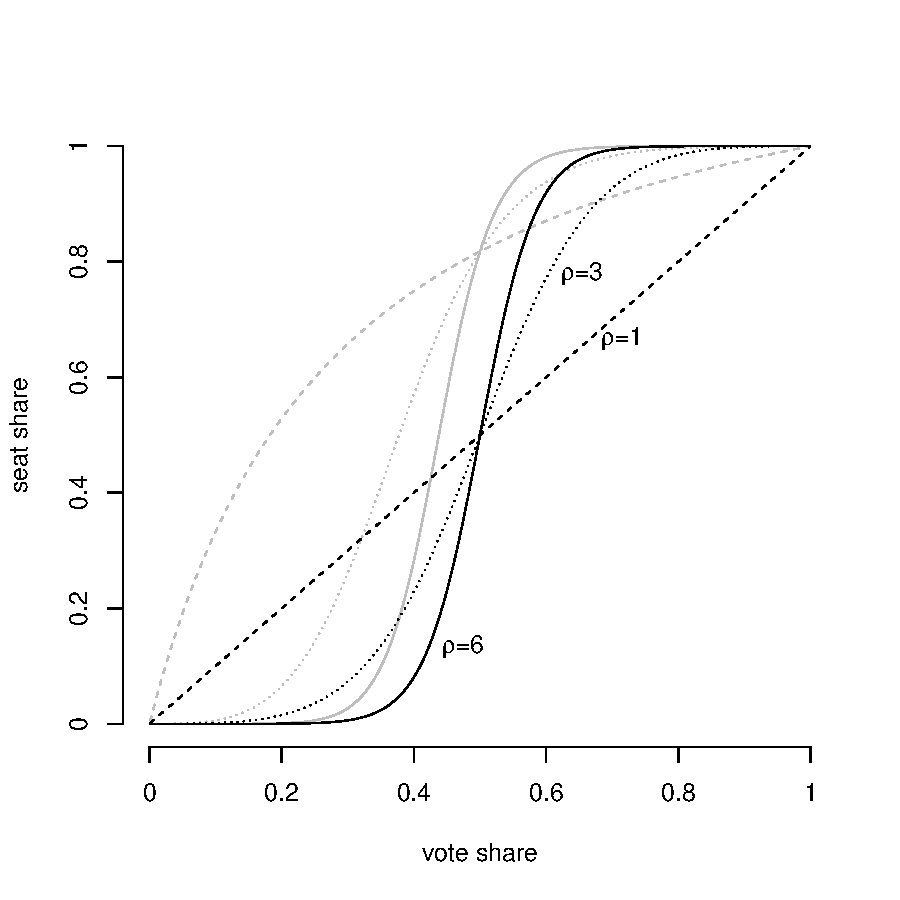
\includegraphics[width=.55\columnwidth]{rhoExample.pdf} 
\caption{Illustration of estimated parameters. Party bias is set to $\lambda=0$ in non-grey lines. Grey lines replicate the colored ones with $\lambda=+1.5$.}\label{F:lambdaRhoEx}
\end{center}
\end{figure}

Non-grey lines lack party bias to illustrate variable responsiveness. A system with $\rho=1$ is perfectly proportional representation, the ideal type against which the evaluation of real districts are often contrasted. It appears as the dotted green diagonal: every party winning $x$\% of the vote gets, precisely, $x$\% of seats. $\rho=3$ characterizes the classic cube law, the red curve over-representing the winner (points above the diagonal). Here a party with 55\% of the vote earns two-thirds of the seats, but with 33\% it earns only one-tenth of the seats. As responsivity grows, the curve gets steeper, until barely crossing the majority threshold suffices to win all the available seats. 

Grey lines replicate the values of $\rho$ just discussed but with $\lambda = 1.5$ added. Bias in favor of the party produces a leftward pull of lines. In other words, a bias-favored party requires less effort to reach the threshold for large-party over-representation. (The grey dotted line demonstrates how, due to logit links in Equation 1, party bias also reshapes the function's trace.)

A multiparty and estimable version of equation 1 \citep{king.1990elRespBiasMultiparty} establishes that party $j$'s ($j=1,2,\ldots,J$) expected seat share is 
\begin{equation}
 E(s_j) = \frac{e^{\lambda_j} * v_j^\rho}{\sum_{m=1}^{J} e^{\lambda_m} * v_m^\rho}
\end{equation}

\noindent with data and parameters indexed to identify the parties. \citep[Another, with application to Argentine federalism, is][.]{calvo.micozzi.govReform.2005} Setting $\lambda_2 = 0$, as done below, forces the remainder $\lambda_{j \neq 2}$ to express party bias with relation to the PRI's ($j=2$ for this party in the dataset). This is convenient to test the presumption of PRI-favoring bias:. if present, $\hat{\lambda}_{j \neq 2}<0$ would result.

A common estimation strategy relies on a time-series of national aggregates (this is what M\'arquez did for eight elections 1991--2012, uncovering substantive anti-PAN bias and high responsiveness). The estimation strategy here, as before, is with state-level data. One disadvantage of the approach is that states have few districts (9.4 on average), and this will amplify the system's responsiveness \citep{taagepera.CubeLaw.1973}. The advantages are many. The approach multiplies observations. This is evident in Figure \ref{F:seatsVotes}, with many points despite reporting three elections only. It holds the actual district structure constant---redistricting in 1997 and 2006 invalidates district comparability before and after. And it takes advantage in the variation of state party systems (this draft fails to take full advantage of this variance, but this could be exploited further). 

\begin{figure}
\begin{center}
  \begin{tabular}{cc}
    (a) & (b) \\
    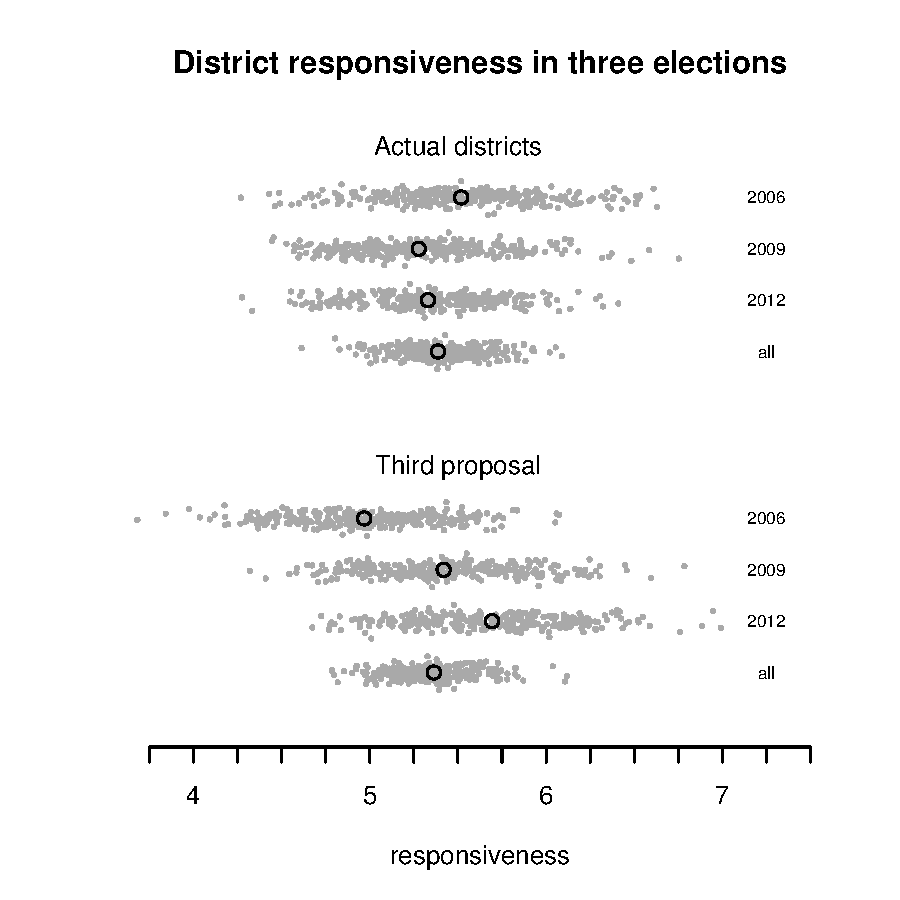
\includegraphics[width=.45\columnwidth]{resp200612s0s3.pdf} &
    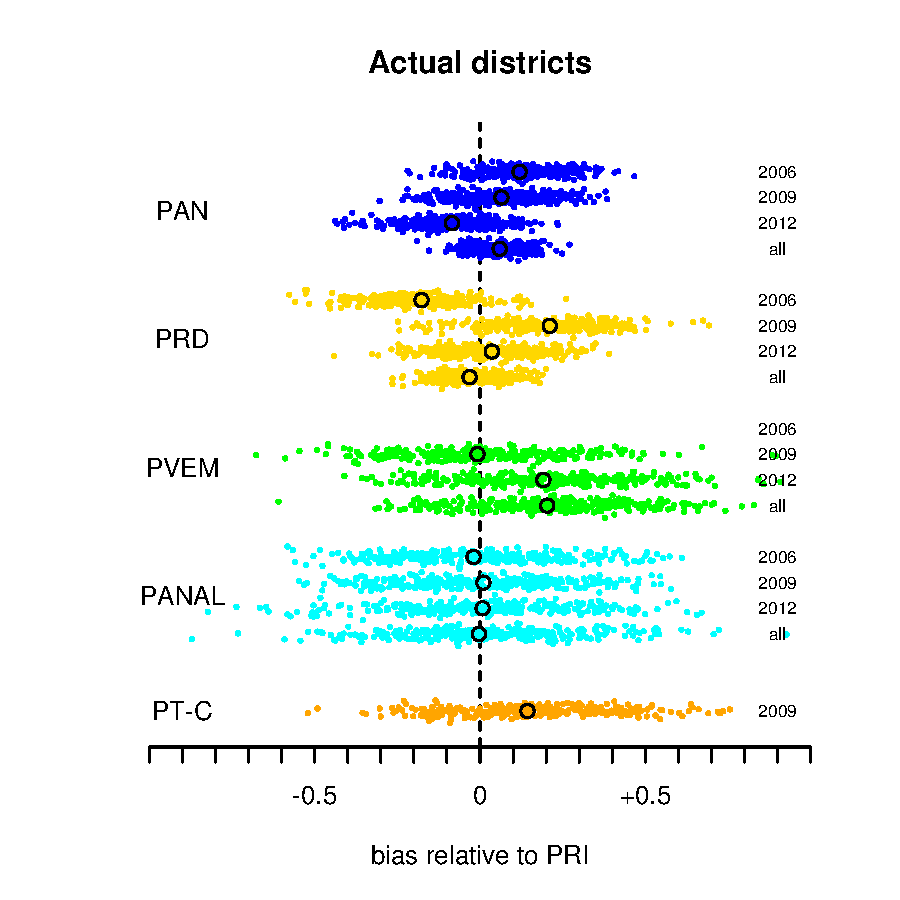
\includegraphics[width=.45\columnwidth]{bias200612s0.pdf} \\
    (c) & (d) \\
    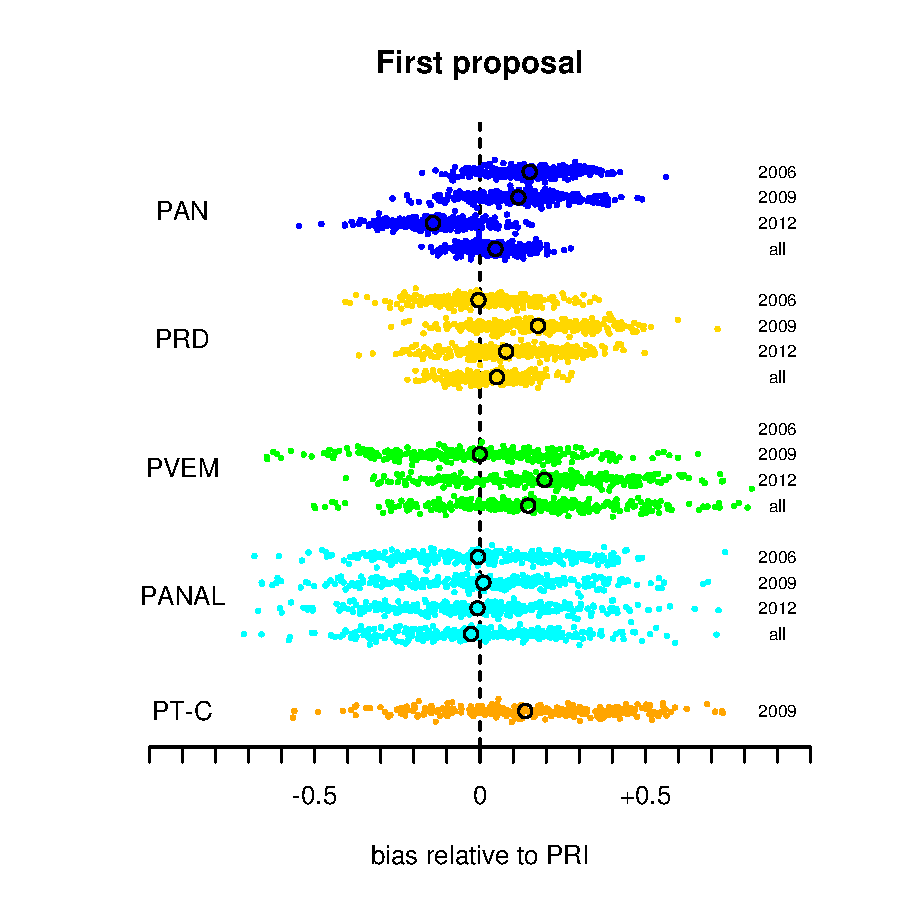
\includegraphics[width=.45\columnwidth]{bias200612s1.pdf} &
    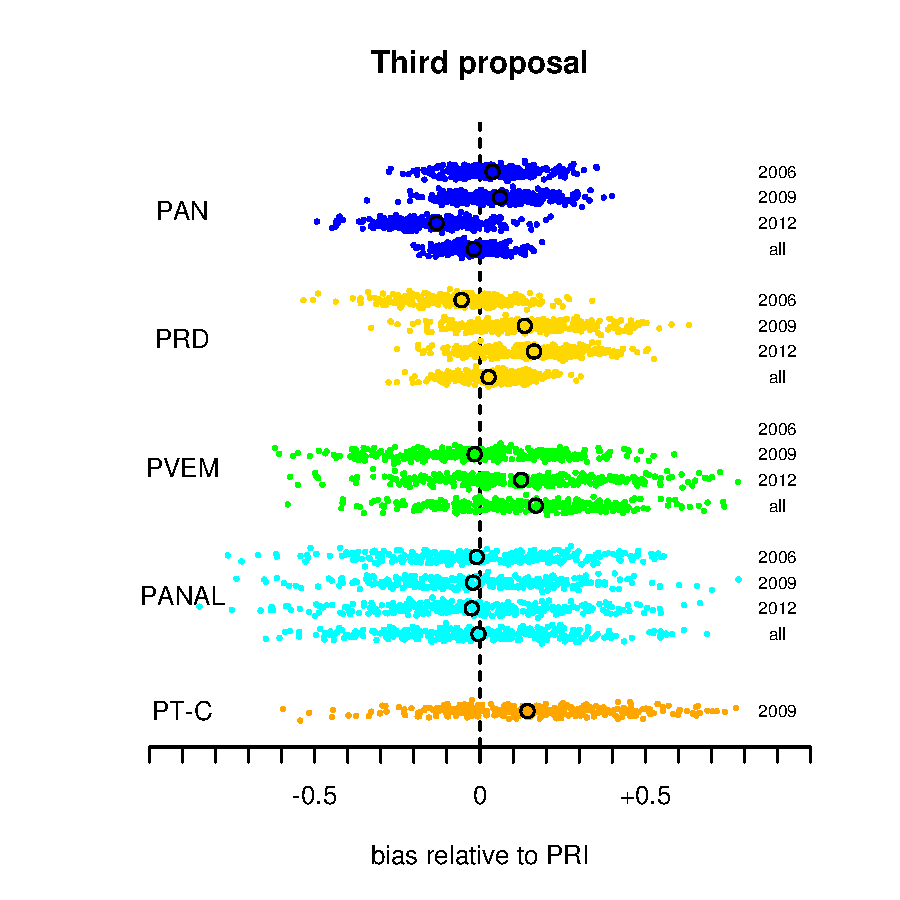
\includegraphics[width=.45\columnwidth]{bias200612s3.pdf} 
  \end{tabular}
  \caption{Redistricting, responsiveness, and party bias. Plots report the posterior sample of model's parameters $\lambda_j$ for four parties and $\rho$, and the median value (black circles).}\label{F:posterior_s0s1s3}
\end{center}
\end{figure}


The  method of estimation is MCMC \citep{jackman.2000}.\footnote{Three chains were iterated 10 thousand times, taking every fiftieth observation of the last 5 thousand to sample the posterior distribution. Convergence was gauged visually with traceplots of the separate chains for each of the model's parameters. Estimation performed with JAGS \citep{jags.cite}, implemented from R \citep{r.cite} using package R2jags \citep{r.r2jags}. Data and code to replicate the analysis can be found at HTTP.} As expected, district responsiveness is extremely high, between 5 and 6 depending on the year selected (the steepest line in illustrative Figure \ref{F:lambdaRhoEx} has $\lambda=6$). Figure \ref{F:posterior_s0s1s3}.a reports point estimates (the black circles are the median of the posterior sample of the responsiveness parameter) for each year separately, all years pooled together, and comparing actual districts to the first and third redistricting proposals. Estimate precision is assessed with the cloud of grey points (technically, it is the full sample of posterior $\rho$s). The redistricting proposal makes little change to district responsiveness, it just makes it slightly more volatile from one election to next. Owing to few districts per state, the estimated responsiveness at the state level ($\hat{\rho} \approx 5.5$) is twice M\'arquez's nationwide ($\hat{\rho} = 2.6$). All three parties experience situations of large party bonus and small party penalty that, to a good extent, cancel each other in the national statistic.

Regarding party bias, signals that are not weak all tend to be accompanied by a good deal of noise, with few exceptions. At the national level, and over a longer haul, M\'arquez discovers bias in favor of the PRI, but mostly in favor of the PRD, and against the PAN, that seems not the product of chance alone. Analysis at the state-level reveals no such biases. As said, Figures \ref{F:posterior_s0s1s3}.b--d express bias relative to the PRI. Although PAN experienced weak signal in its favor in the whole 2006--12 period, a fair density of the blue cloud is, in fact, negative. PRD vs.\ PRI bias is clearly centered at zero in the full period. The left did experience significant bias in isolated years: against in 2006, in favor in 2009. Perhaps voters who strategically abandoned the hopeless PRI presidential candidate in 2006 to vote for L\'opez Obrador did not also endorse the PRD's congressional candidates. No other year for no other party reveals any bias unaccompanied by much noise.

% \section{Malapportionment and margin}

% \begin{figure}
% \begin{center}
%   \begin{tabular}{cc}
%     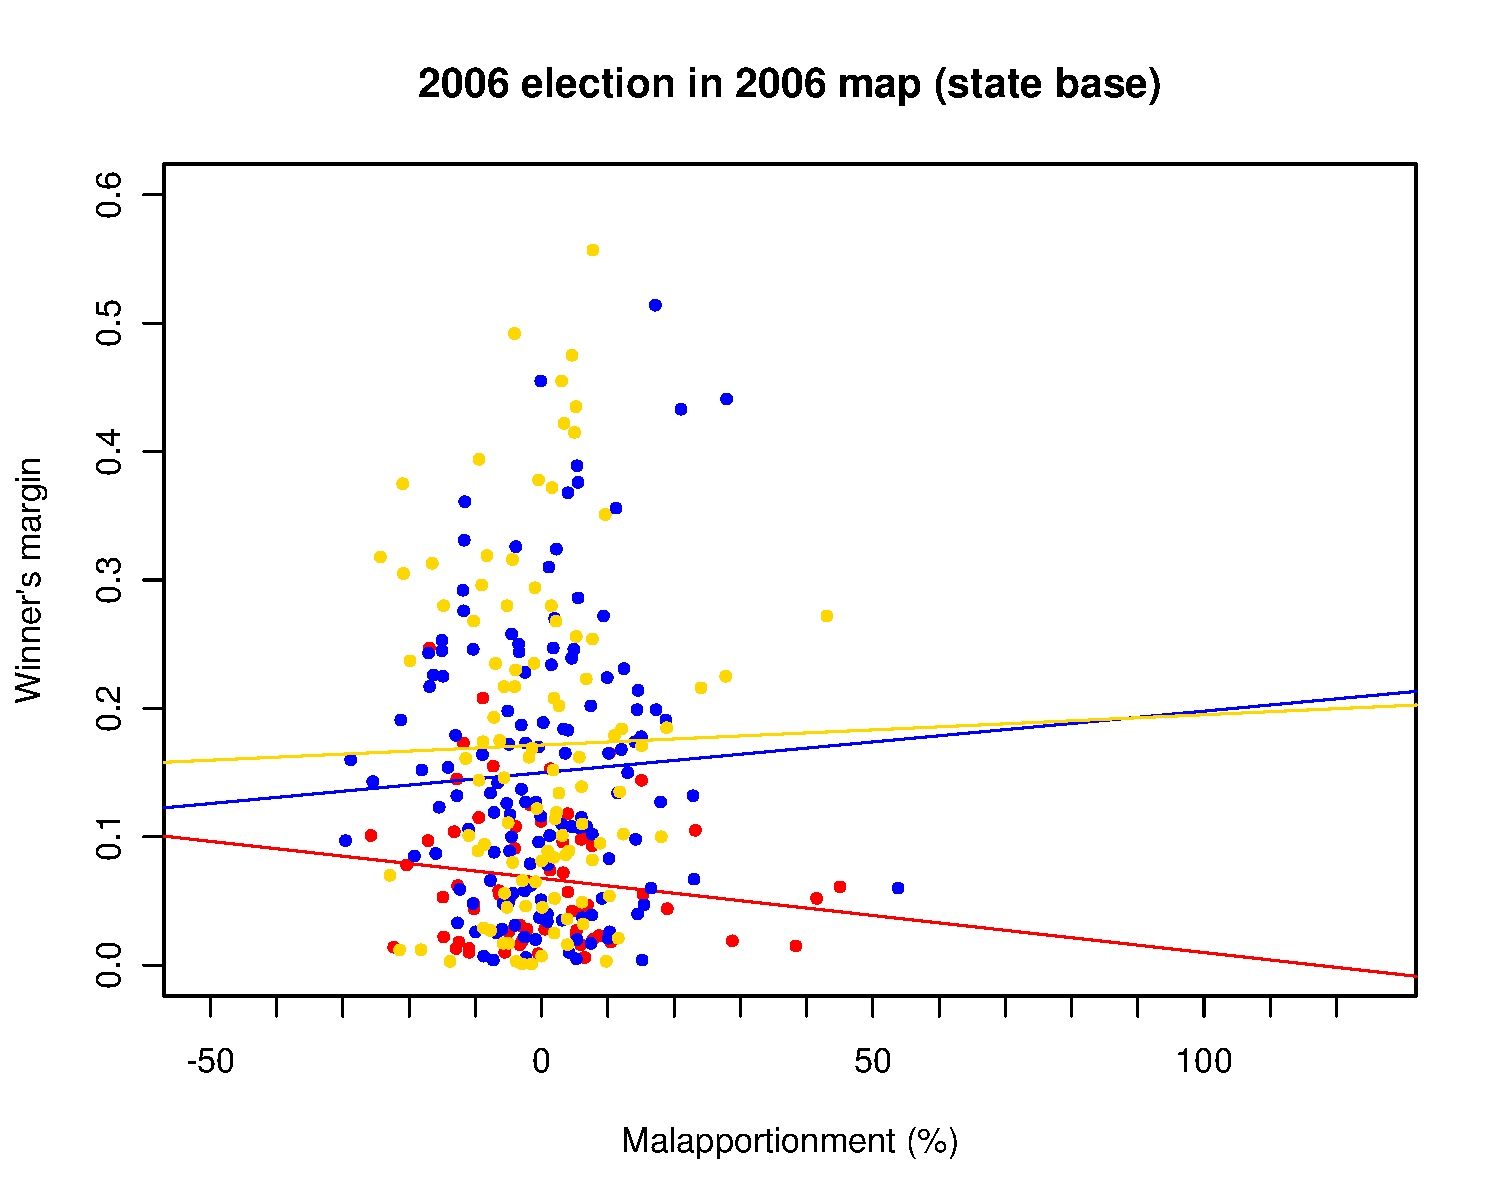
\includegraphics[width=.4\columnwidth]{malmg2006d0sta.pdf} & 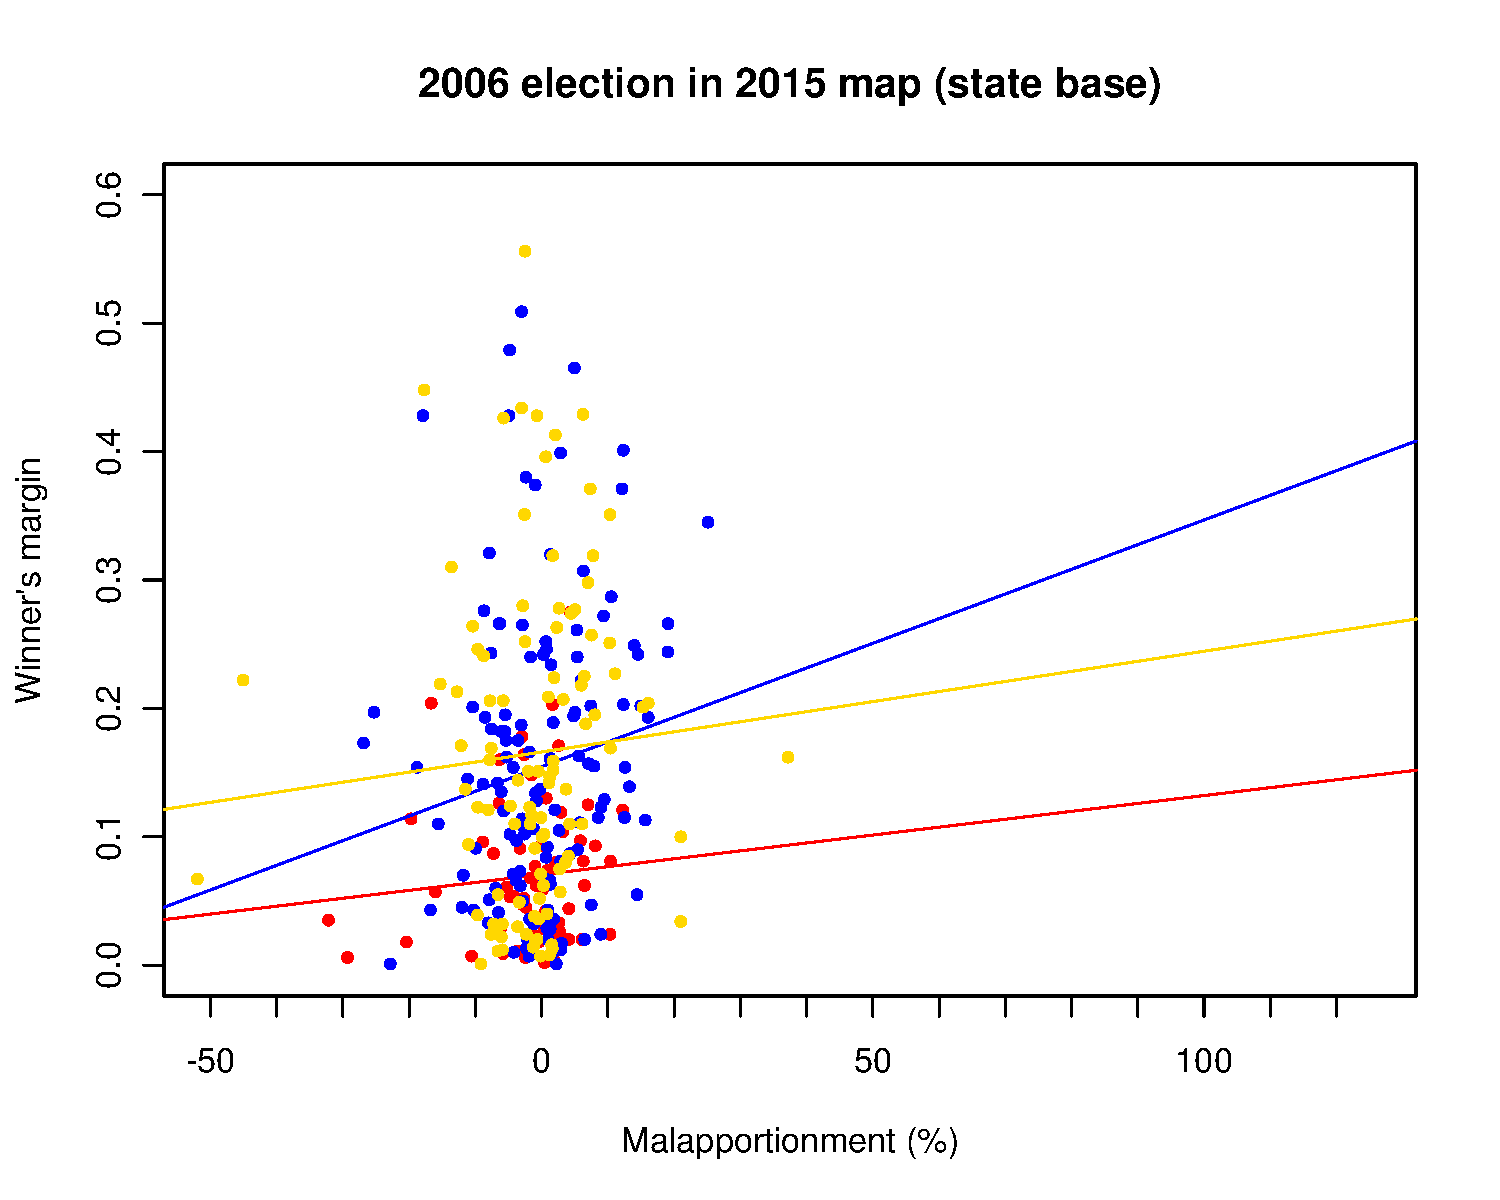
\includegraphics[width=.4\columnwidth]{malmg2006d3sta.pdf} \\
%     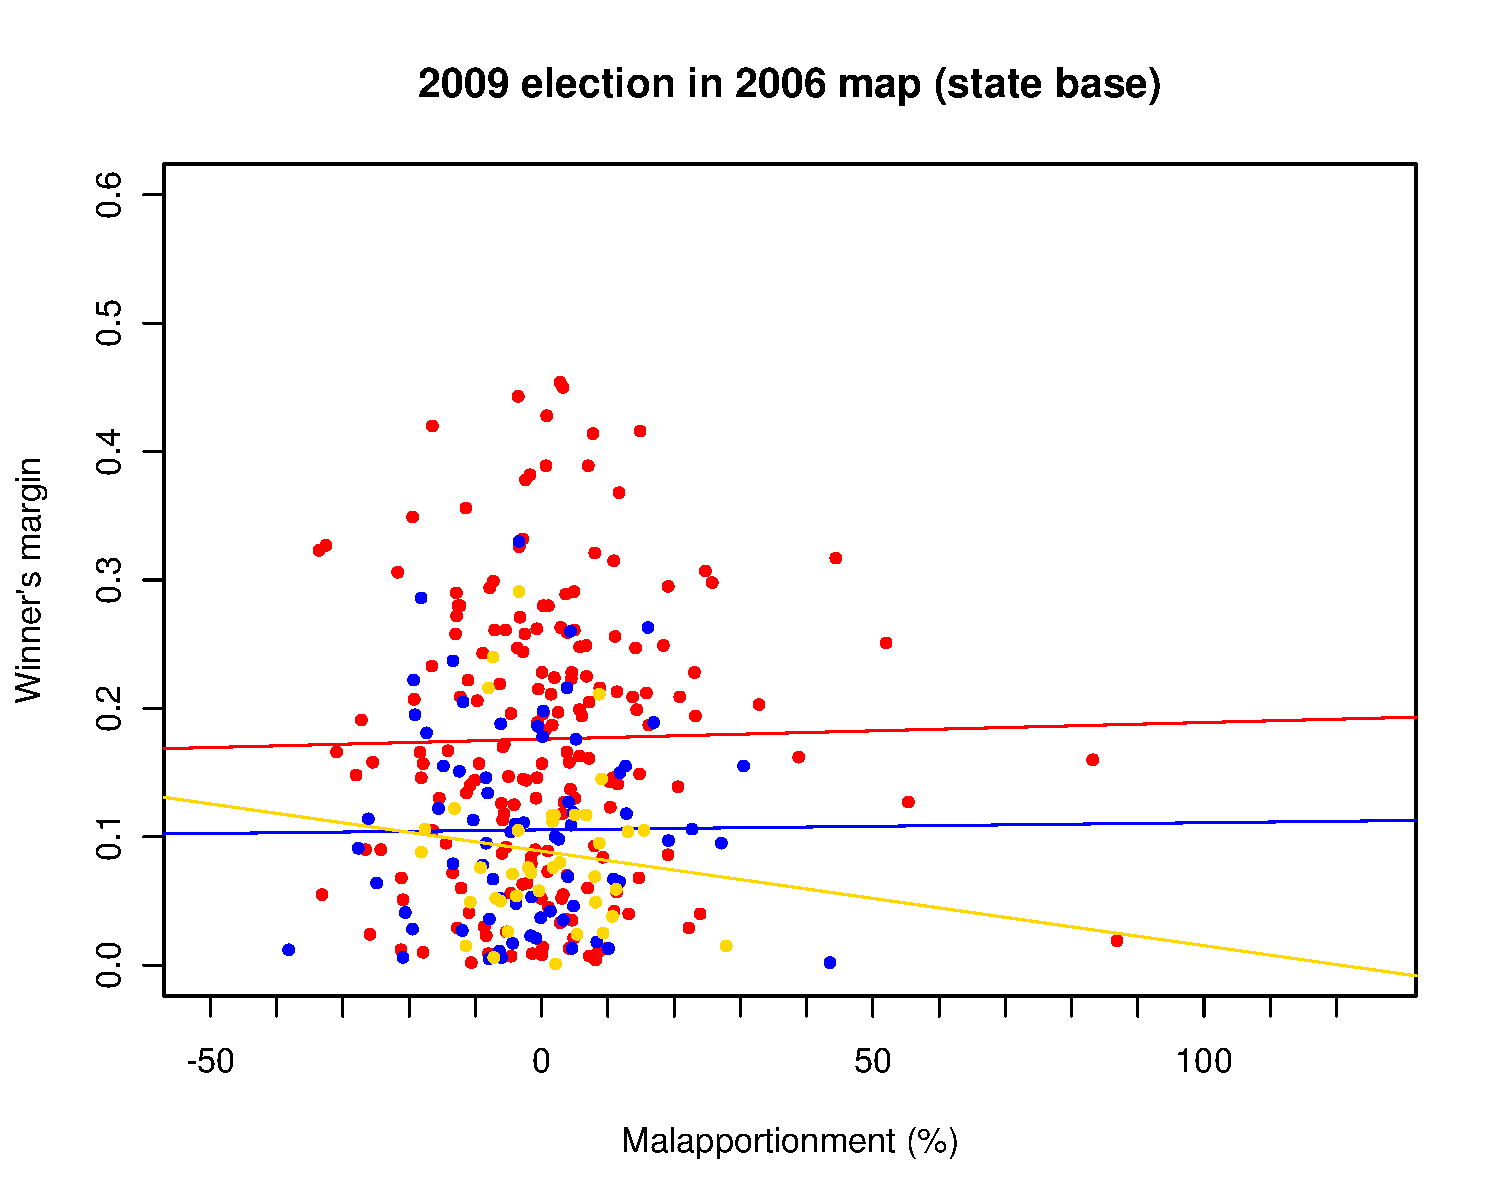
\includegraphics[width=.4\columnwidth]{malmg2009d0sta.pdf} & 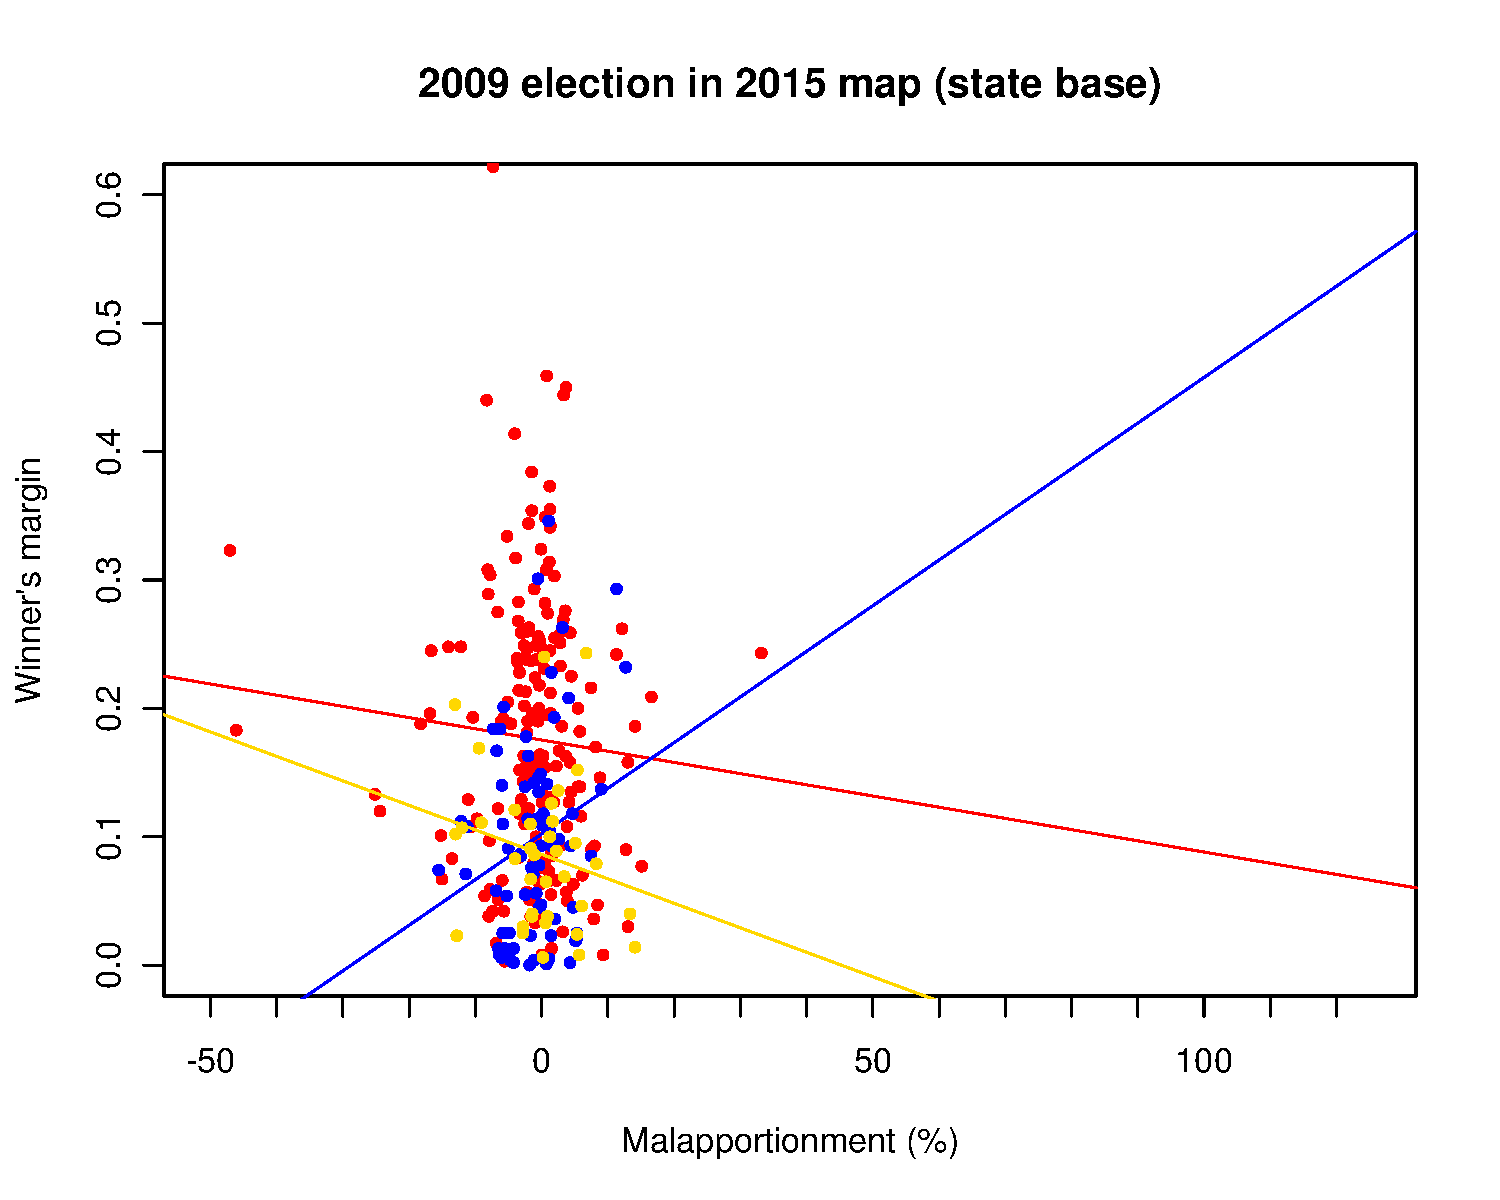
\includegraphics[width=.4\columnwidth]{malmg2009d3sta.pdf} \\
%     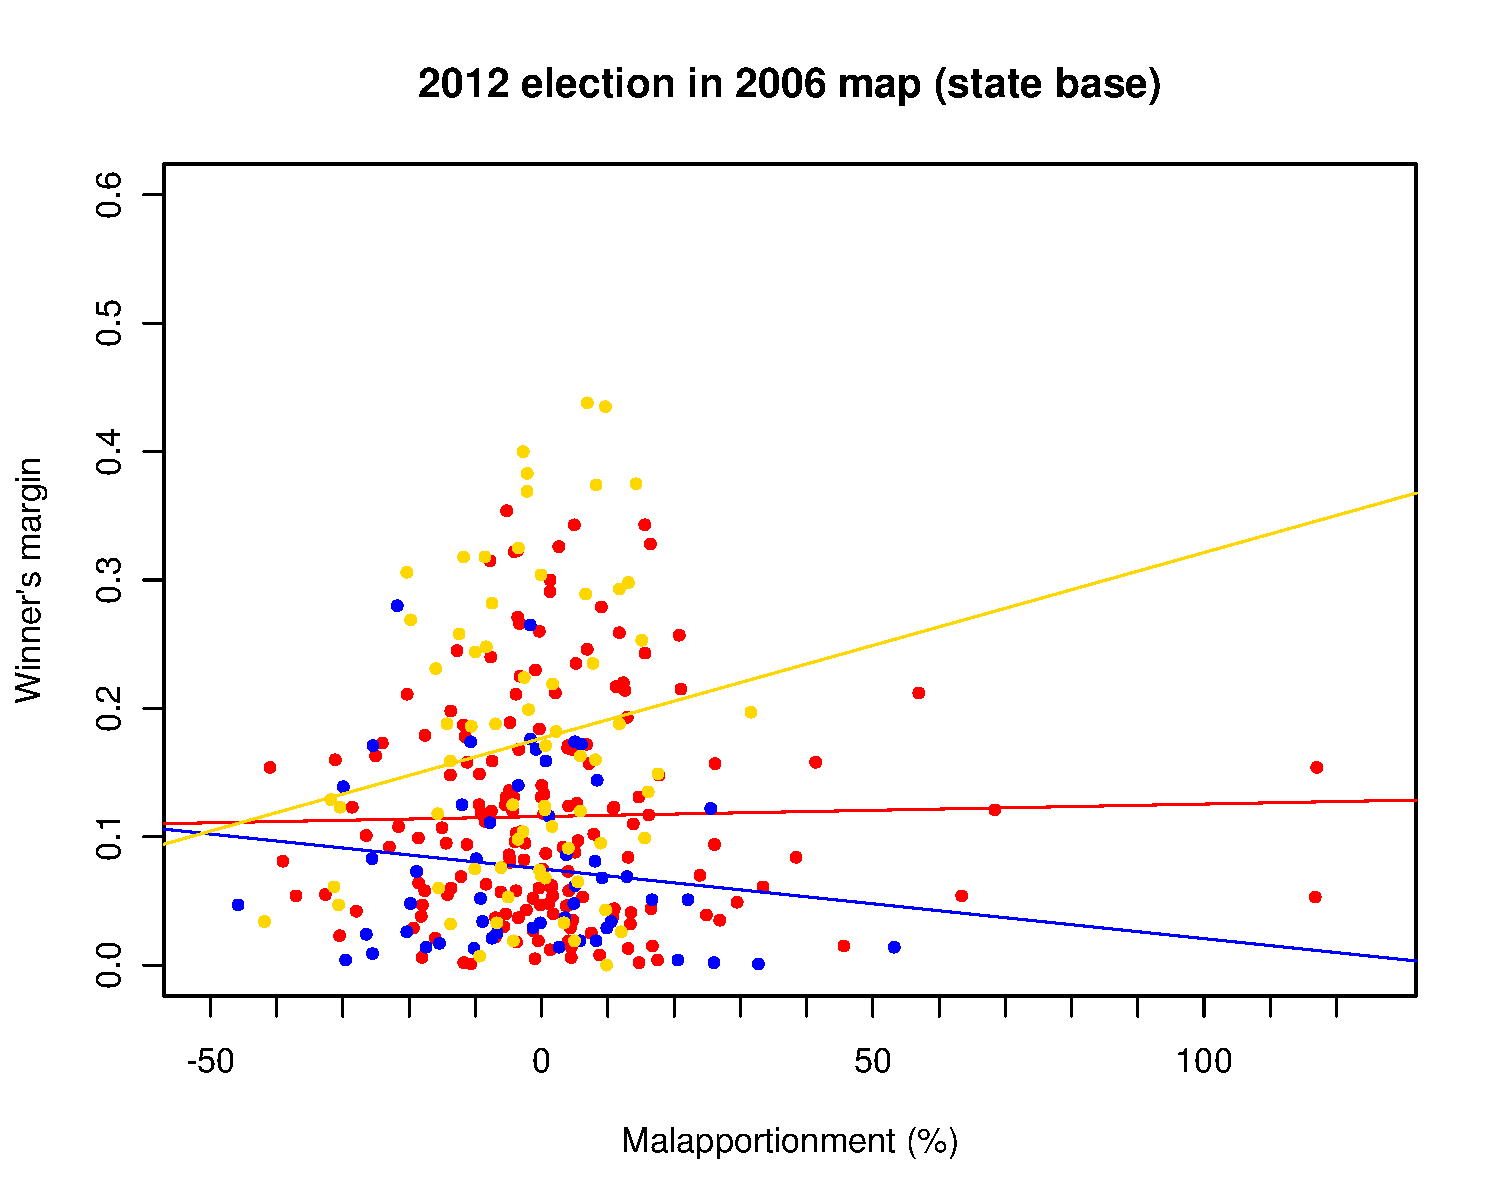
\includegraphics[width=.4\columnwidth]{malmg2012d0sta.pdf} & 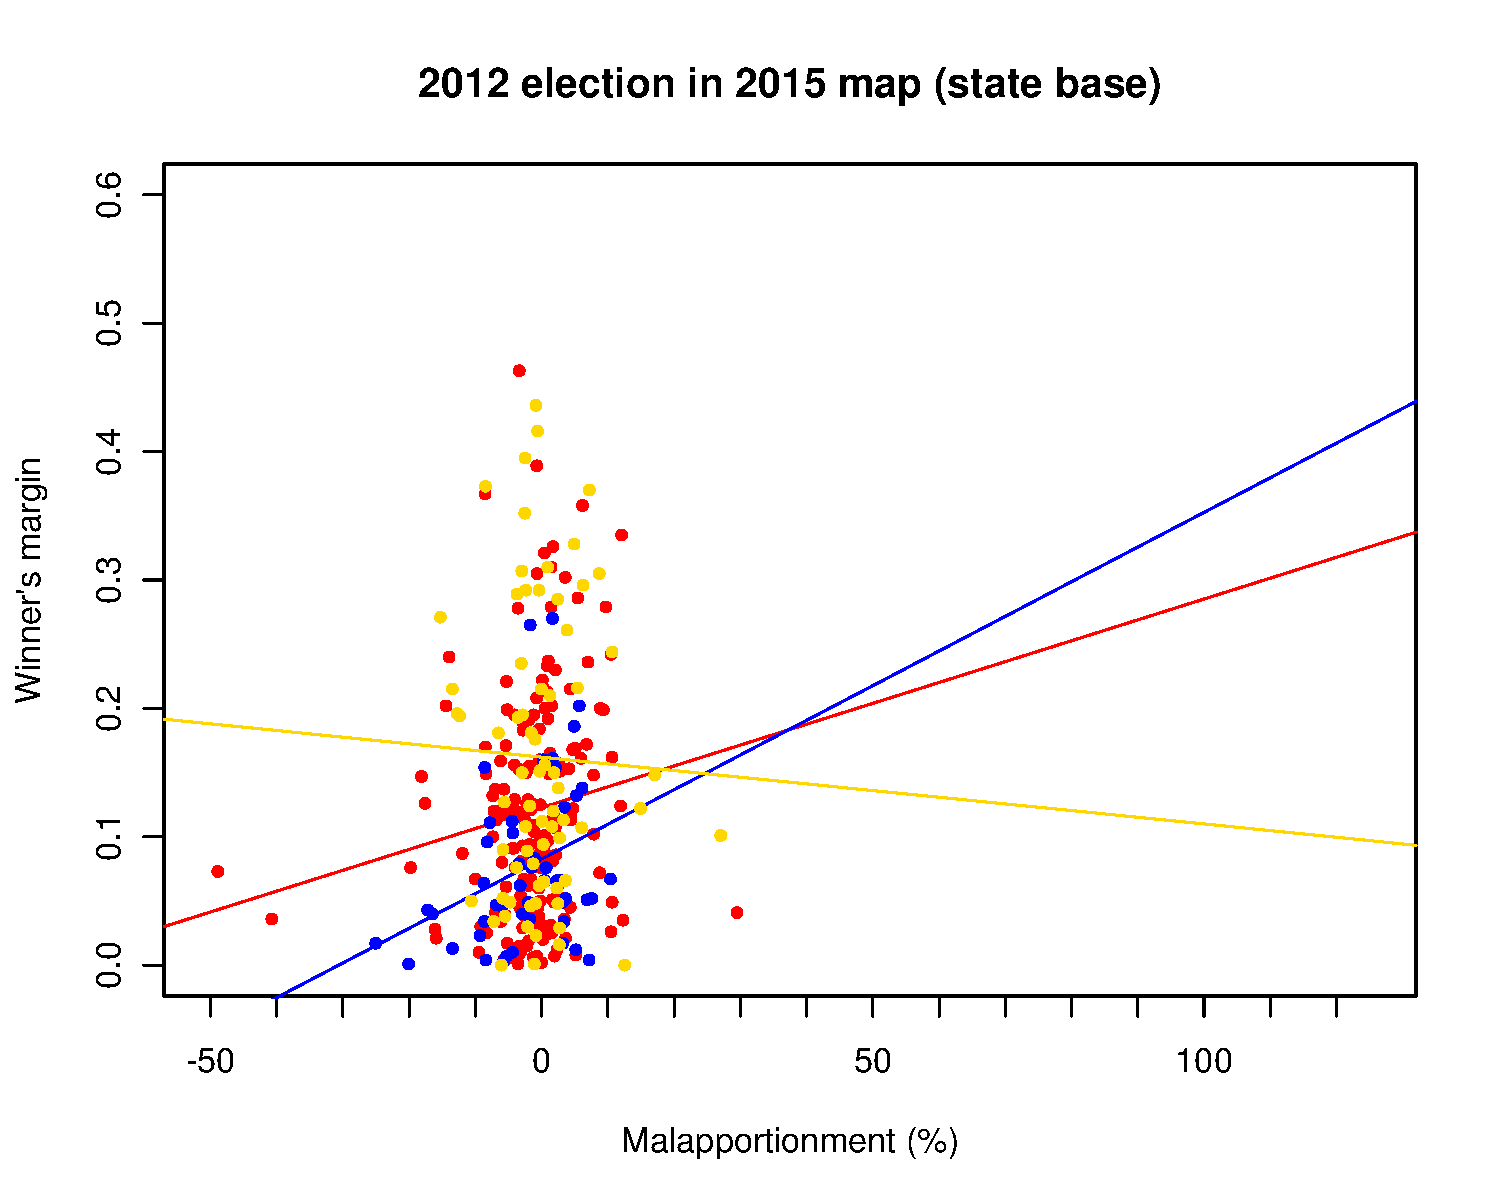
\includegraphics[width=.4\columnwidth]{malmg2012d3sta.pdf} \\
%   \end{tabular}
%   \caption{Vote margin and malapportionment (compared to state averages)}\label{F:malmgsta}
% \end{center}
% \end{figure}

% \begin{figure}
% \begin{center}
%   \begin{tabular}{cc}
%     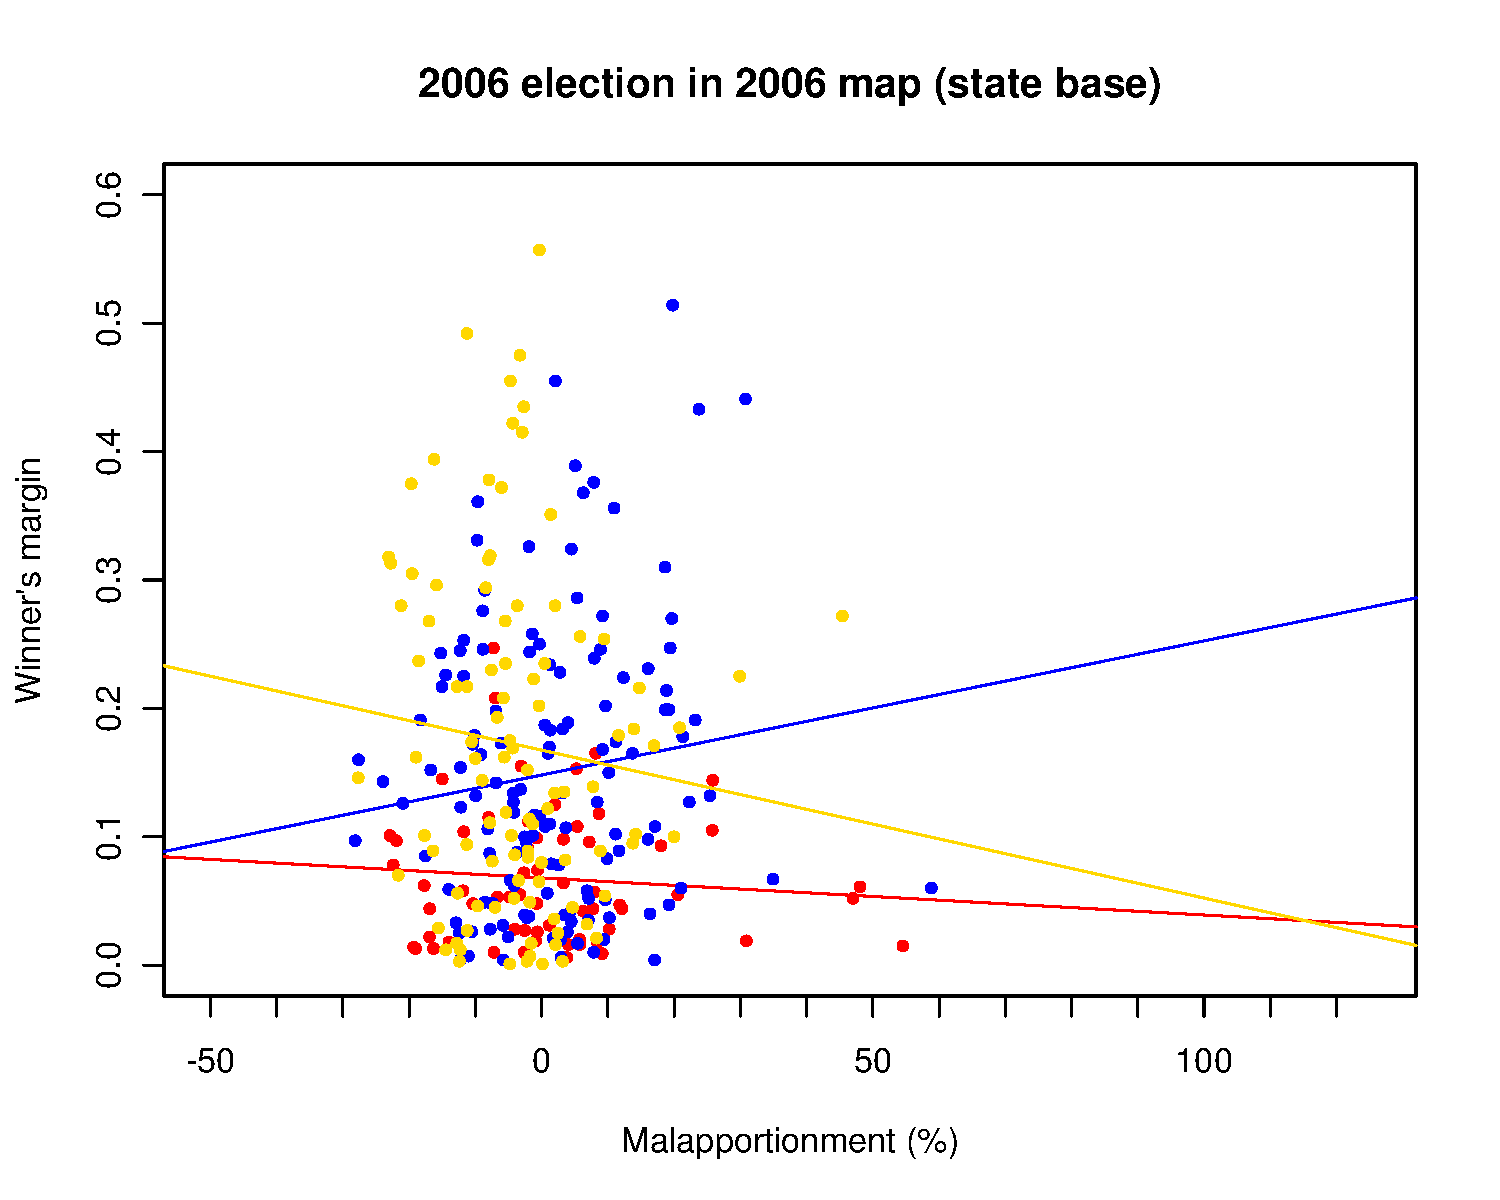
\includegraphics[width=.4\columnwidth]{malmg2006d0nat.pdf} & 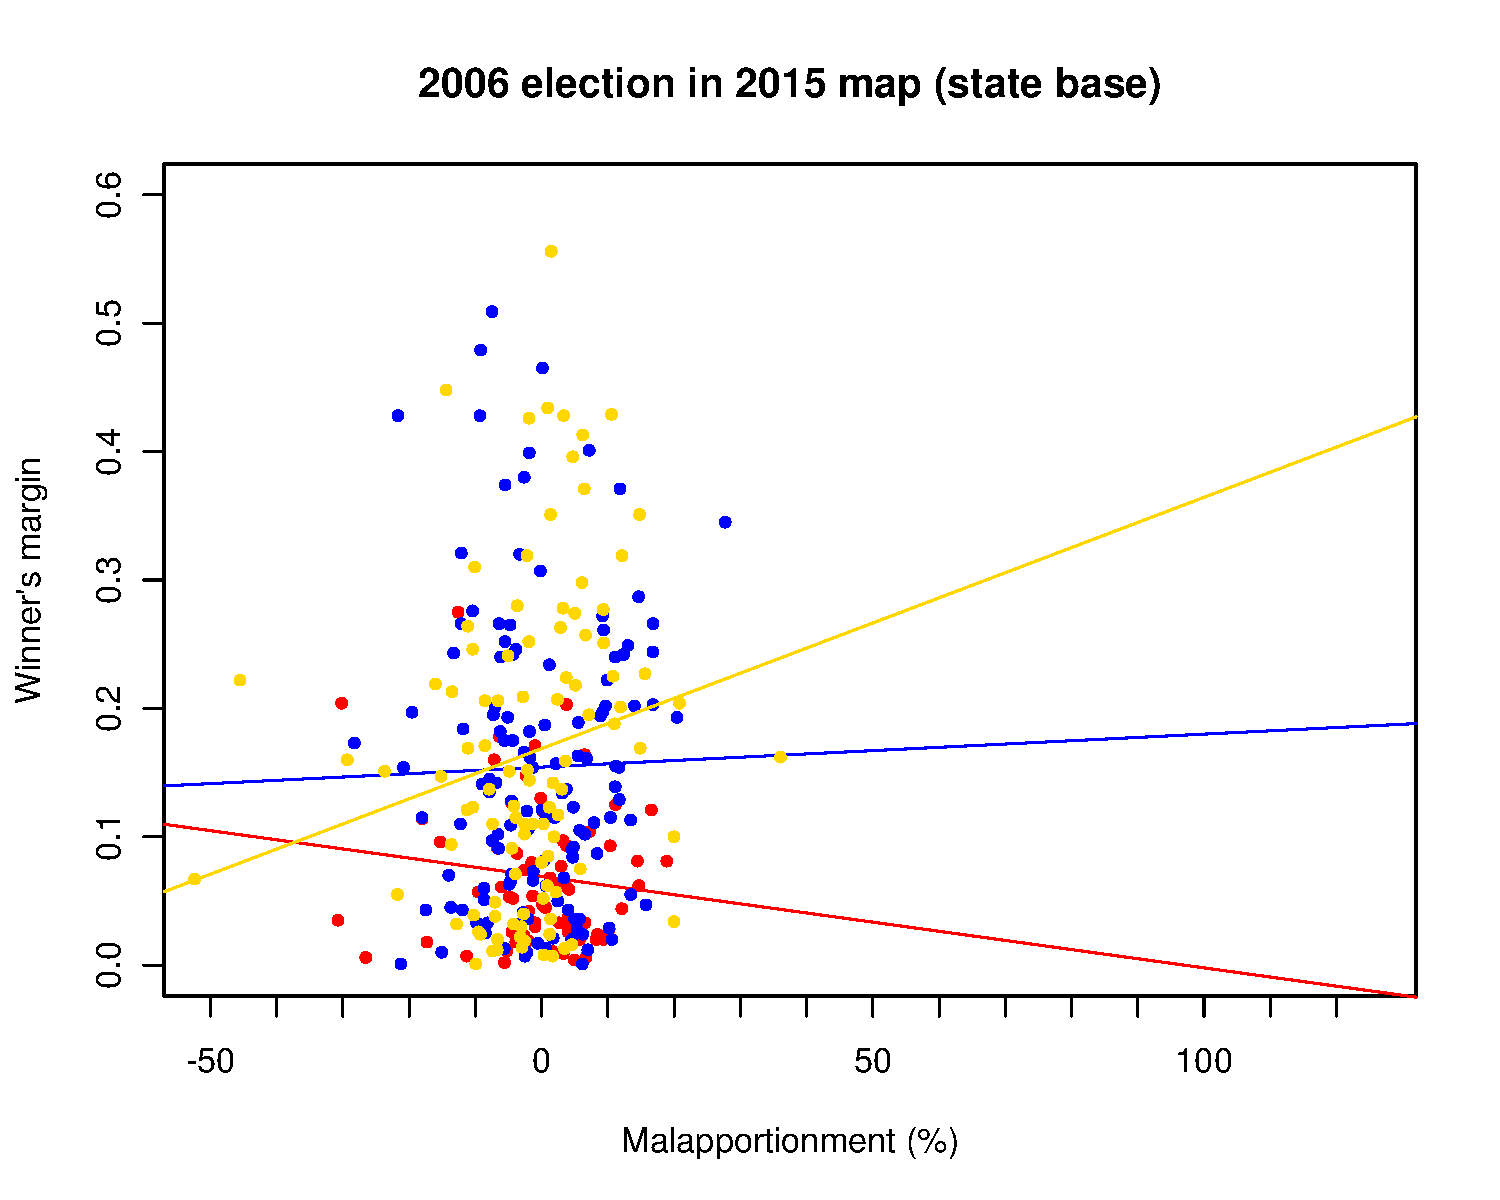
\includegraphics[width=.4\columnwidth]{malmg2006d3nat.pdf} \\
%     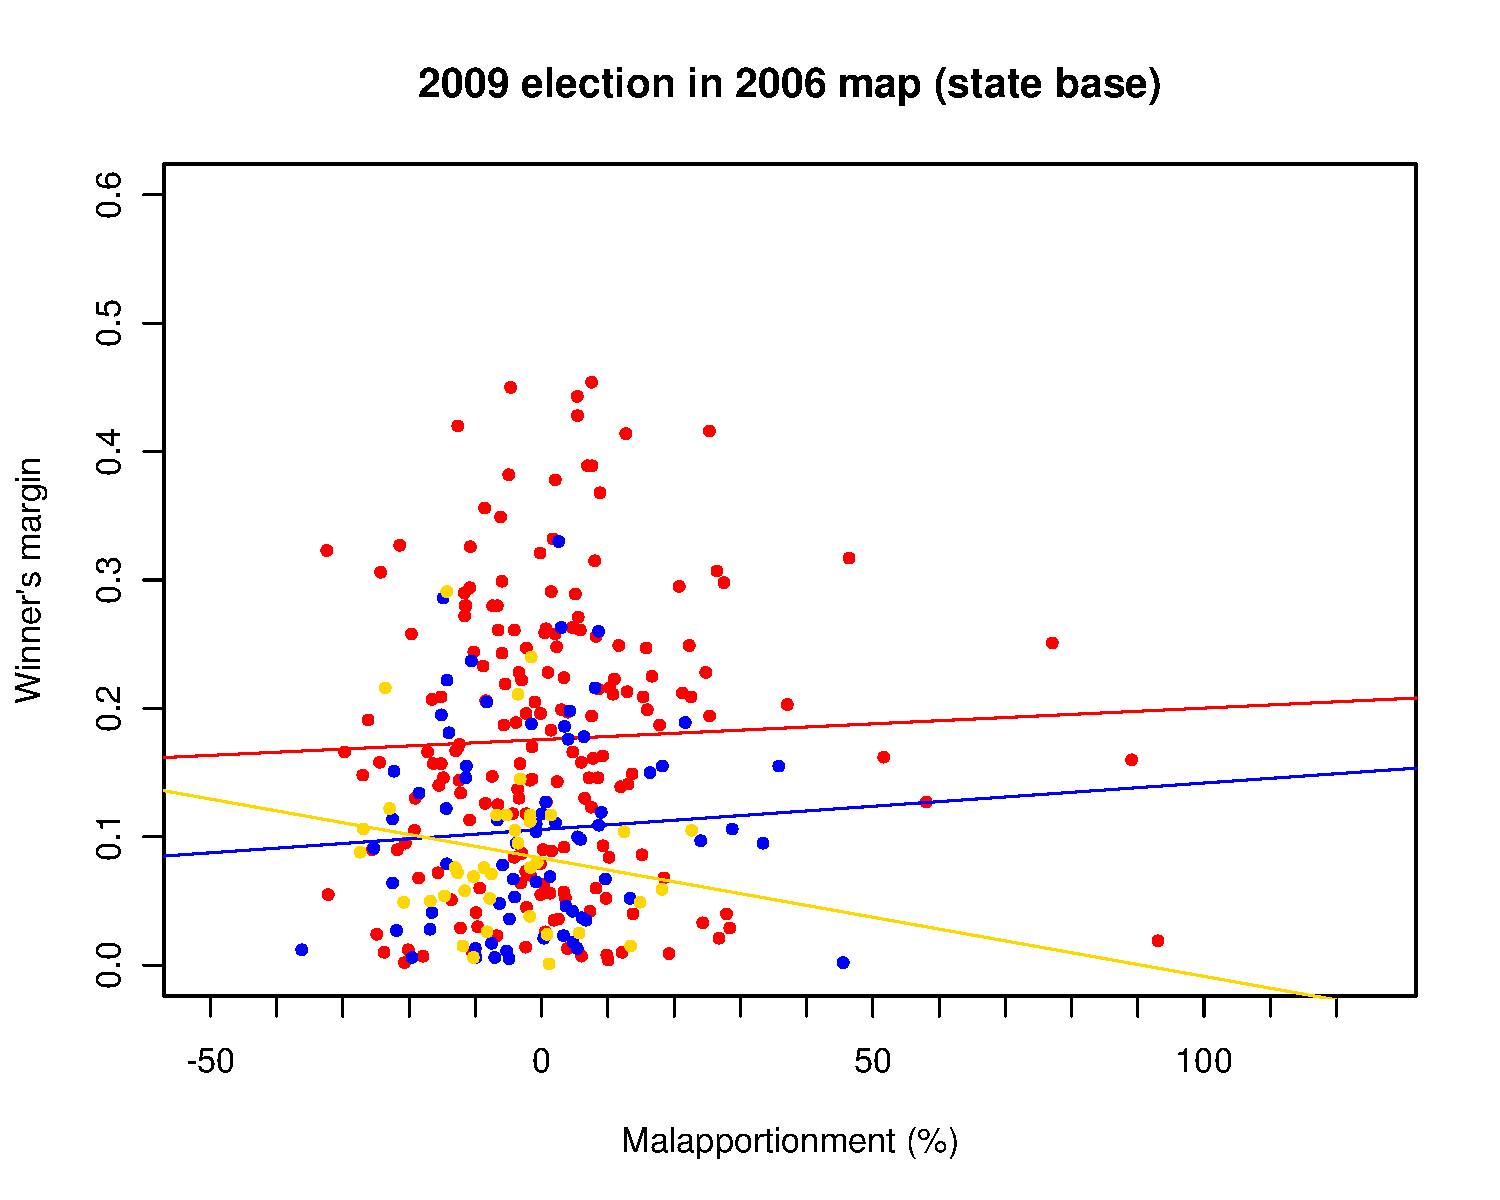
\includegraphics[width=.4\columnwidth]{malmg2009d0nat.pdf} & 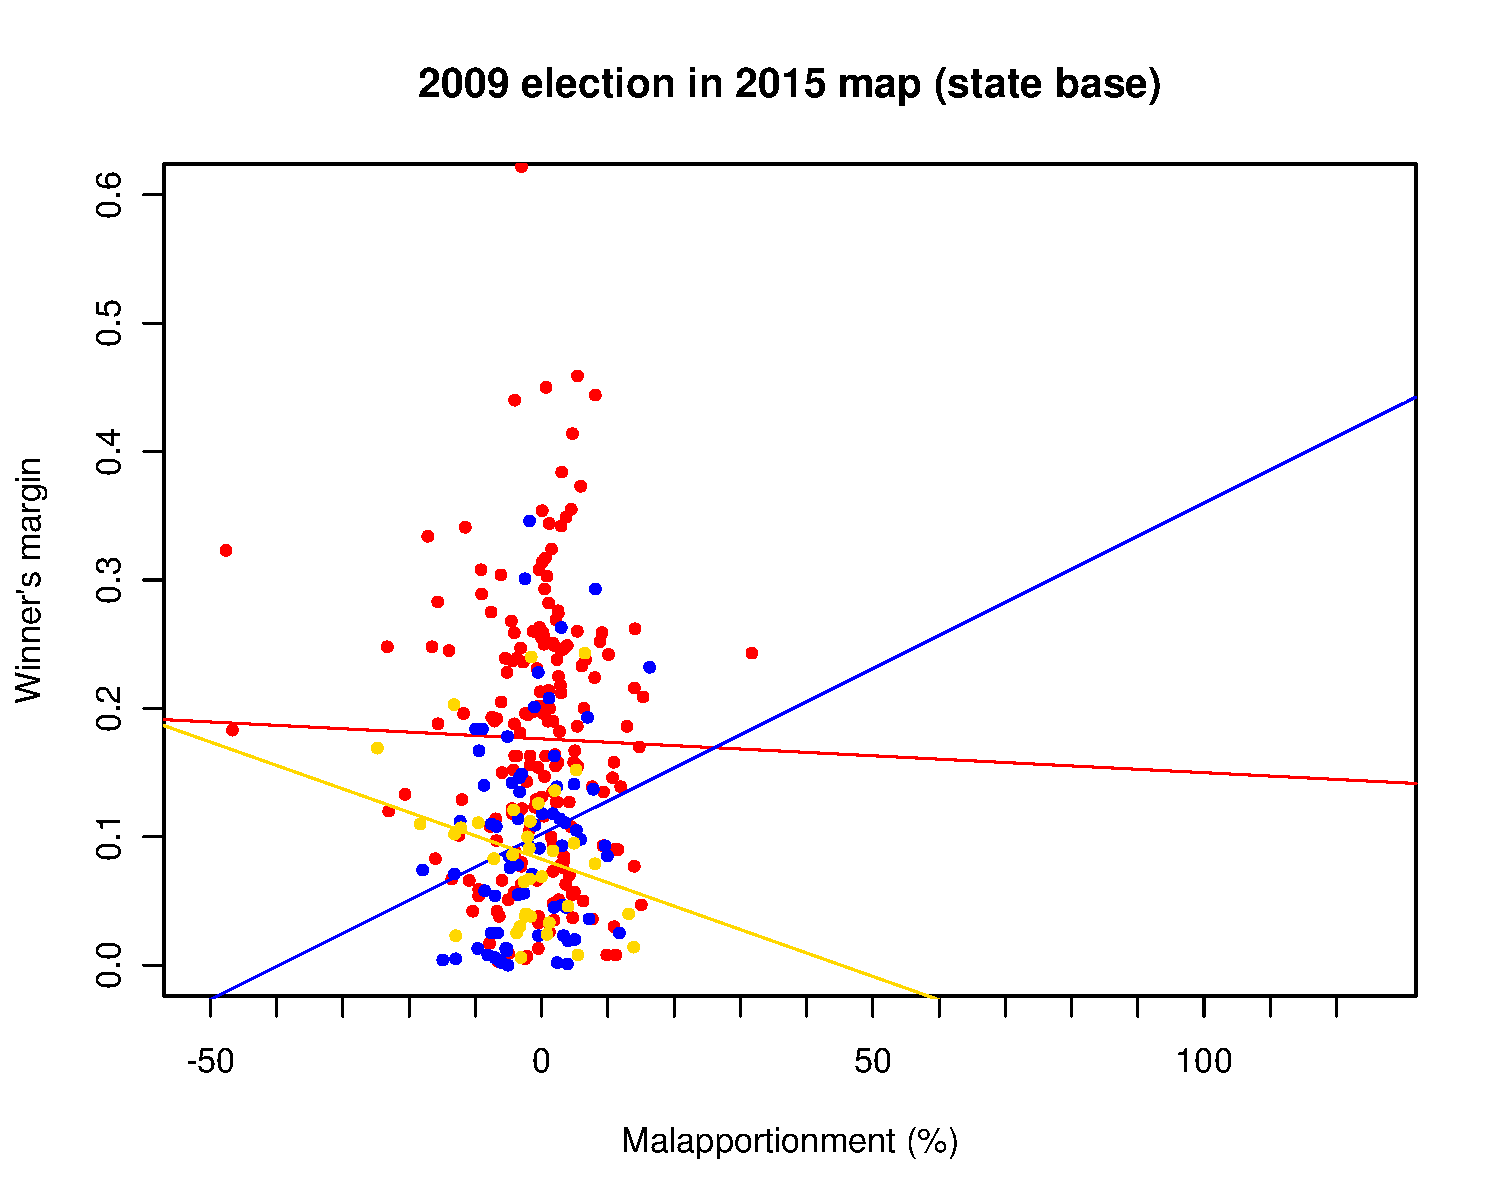
\includegraphics[width=.4\columnwidth]{malmg2009d3nat.pdf} \\
%     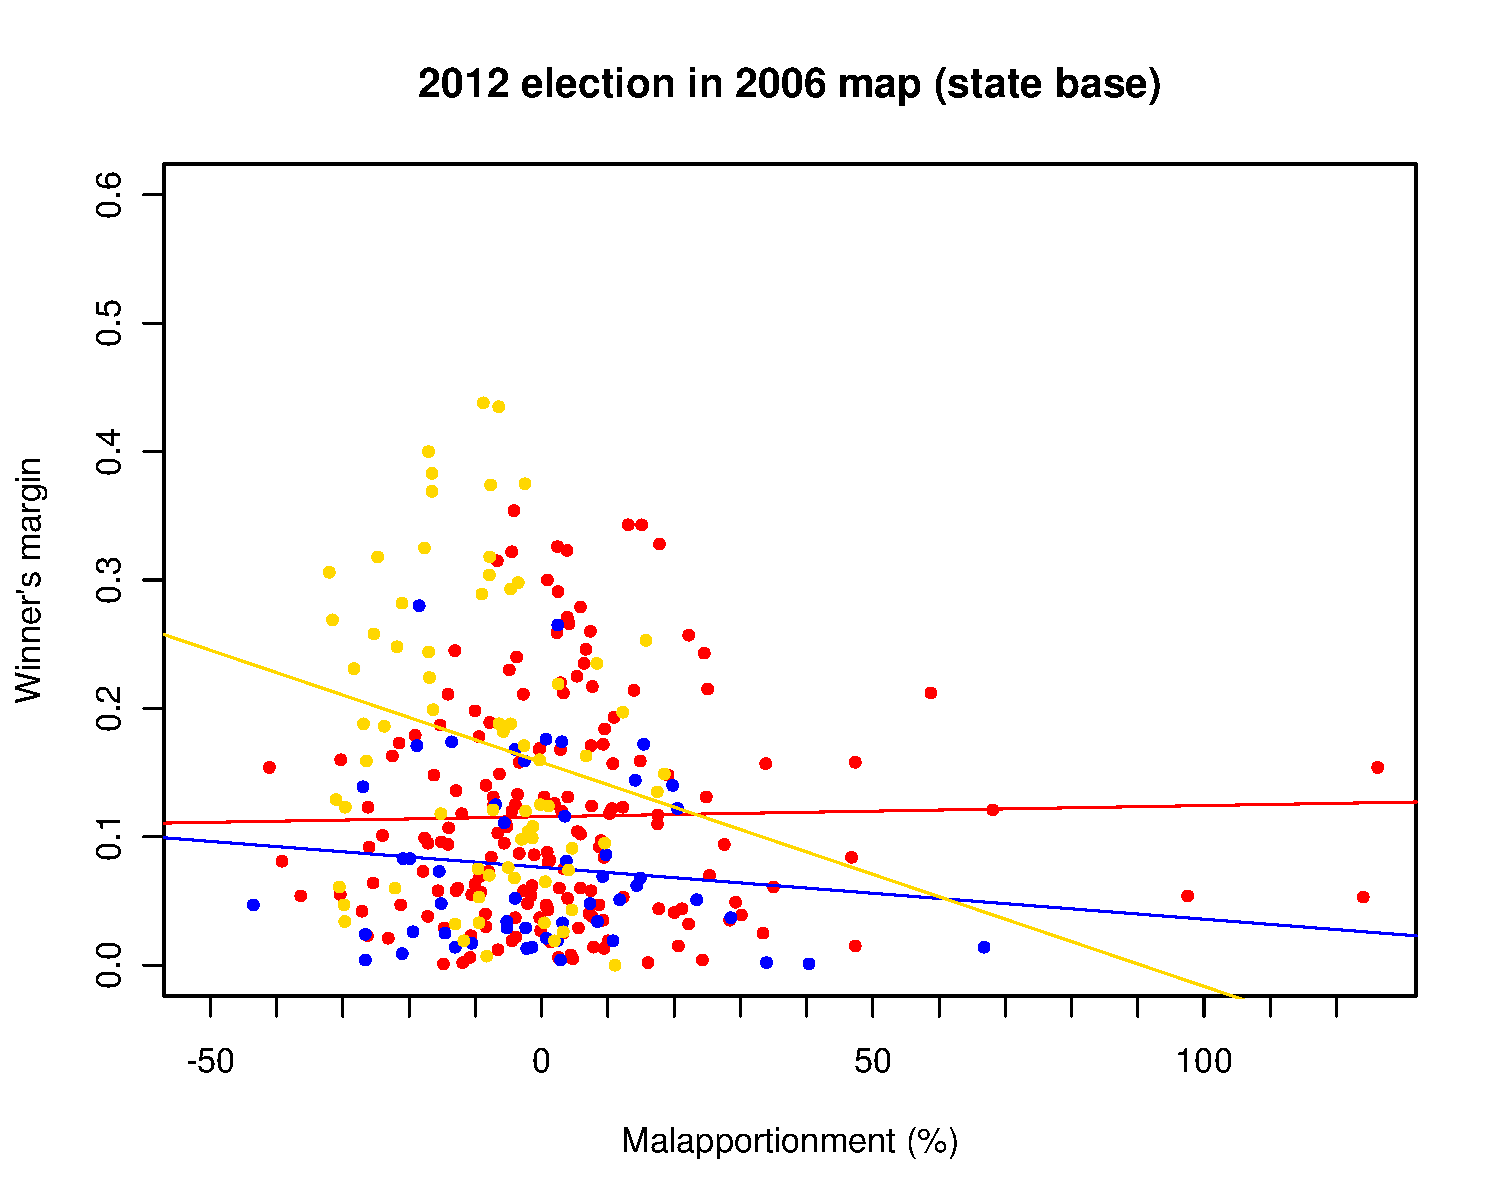
\includegraphics[width=.4\columnwidth]{malmg2012d0nat.pdf} & 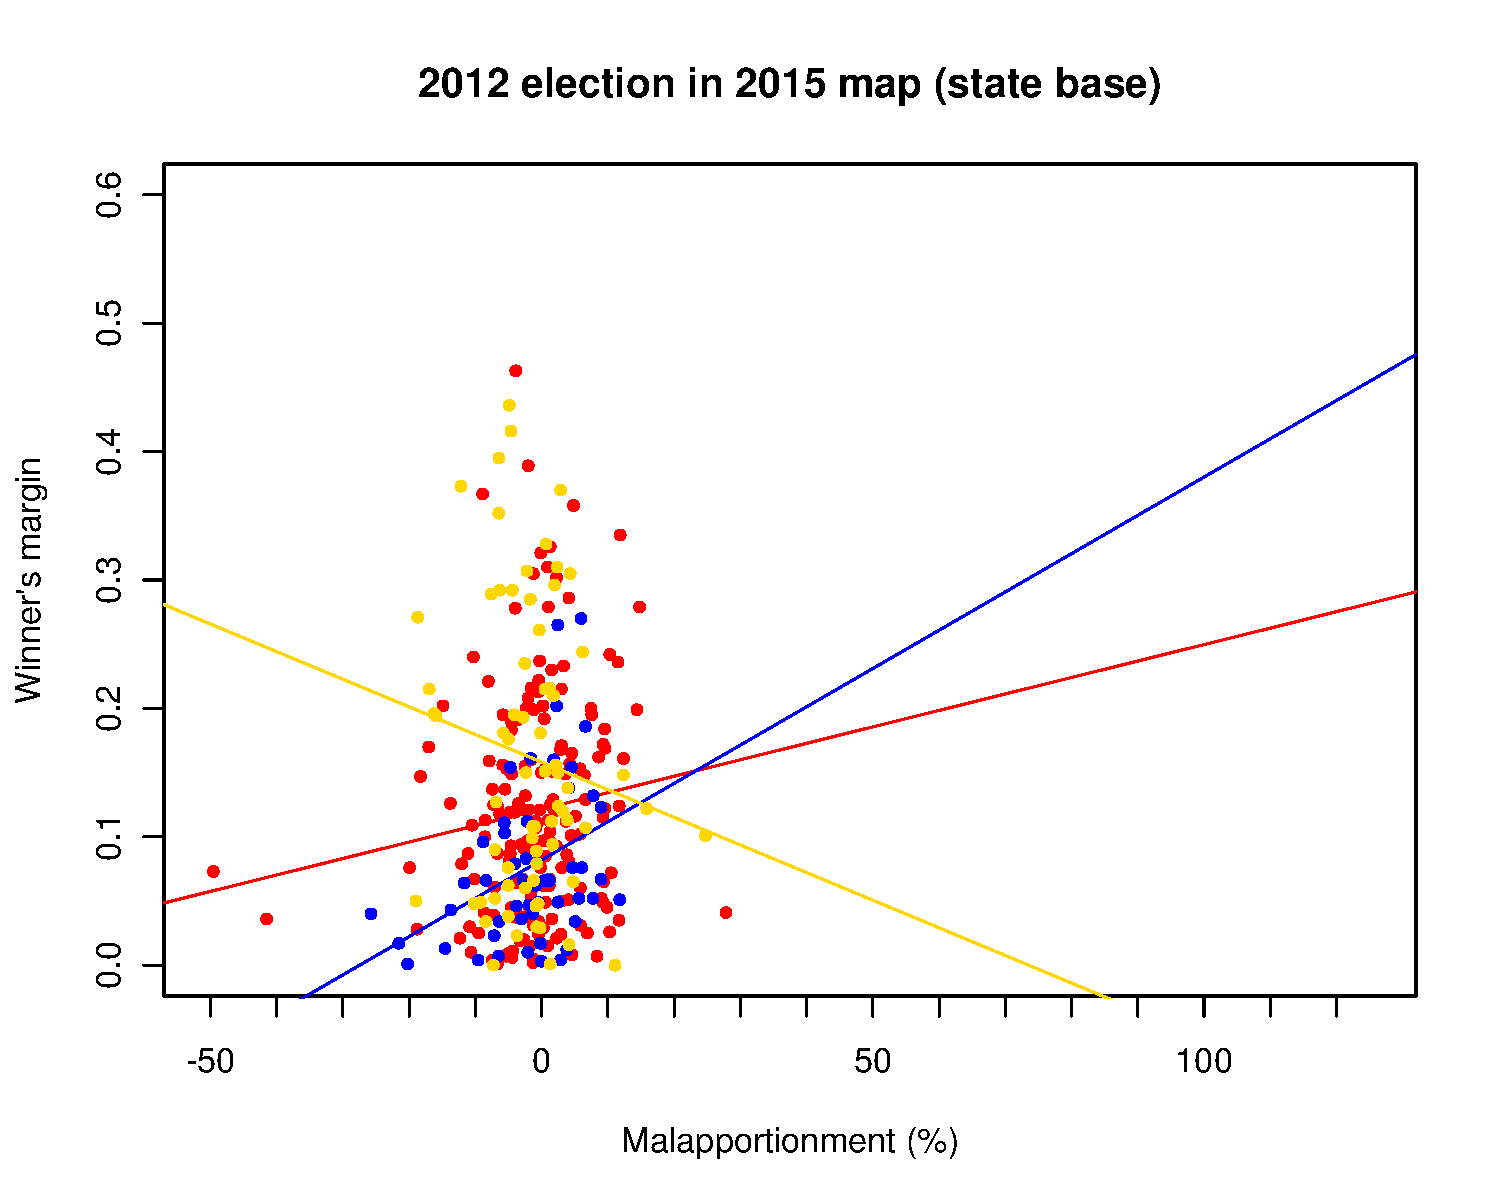
\includegraphics[width=.4\columnwidth]{malmg2012d3nat.pdf} \\
%   \end{tabular}
%   \caption{Vote margin and malapportionment (compared to national average)}\label{F:malmgnat}
% \end{center}
% \end{figure}

% Plots in Figures \ref{F:malmgsta} and \ref{F:malmgnat} 

\section{Conclusion}

** To be written **

Mexico's federal districts exhibit no party bias when analyzed at the state level. Big system responsiveness, typical of first-past-the-post system in units with few federal districts, is associated with the districts. So PRI's tendency to be over-represented more than PAN and PRD, and the PRI's winning of a couple extra seats with the redistricting proposal is not the product of partisan bias. If the PRI wins more this is due to its status as the largest party in more states that the other two major parties combined. 

%Comment [Alejandro]: 

%It seems that what the above paragraph suggests is that the check and balance system (automation + partisan interaction) of Mexico's redistircting process works... A big question is if this type of model (partisan interaction, automation and openness) is something that we would like to see replicated elsewhere (i.e. US or any other country that goes through similar processes) or in the next Mexican federal or local redistricting process that will take place in the next decade... 

% We still need to analyze with closer detail the dynamic of partisan interaction and we might want to simulate what would happen with effective self-interetsed players. I assume we  we would like to understand how this interaction might develop in the near future  and its effects on representation for potential use in other countries... 

% These are some of the questiones I had in the Conclusions section of the APSA2014Paper Word Version:

% Why did parties choose to postpone the approval of the 2013-redistricting plan? Introducing legislative reelection, a higher stake for automated redistricting? Uncertainty generated by the effect of changing the boundaries in the next 4 legislative elections? Who wins and who looses by staying with the status quo (2005 maps)?  Were the adopted neutral redistricting criteria politically neutral?  Were the plans produced algorithmically, in fact, optimal with respect to the selected criteria? How did partisan counterproposals differ from the bureaucratic solution?  What influence did parties have on the final proposed plan?



\section*{Appendix} 

\subsection*{Elasticity}

% Adding more election cycles will improve the estimates. Two points now for each line as of now. 

How elastic a district is to a party's statewide (nationwide?) vote swings is interesting. Elasticity should shape redistricting preferences. A district is highly elastic for the PAN when small shifts in the party's vote statewide correspond to sharp district vote hikes. It is inelastic when it corresponds to more modest district vote changes. Negative elasticity is even conceivable, the district vote growing when the rest of the state shrinks. Local effects on mobilization and voting can move against state effects. If every section in the district is a microcosm of the state's electorate, unit elasticity ensues. 

The measure regresses a party's three-year vote change in the section $\Delta_s$ on the the parent state vote change $\Delta_e$ thus:  

\begin{equation}
\Delta_s = \sum\limits_{d=1}^{D_e} \alpha_d + \beta_d \Delta_e.
\end{equation}

\noindent Fixed effects for each district are considered, fitting separate $\alpha_d$ and $\beta_d$ regression coefficients for every district (indexed $d$). The model is estimated for every state separately because doing it nationwide involves too many sections (67k) and parameters (600) for my machine. 

\begin{figure}
\begin{center}
  \begin{tabular}{cc}
    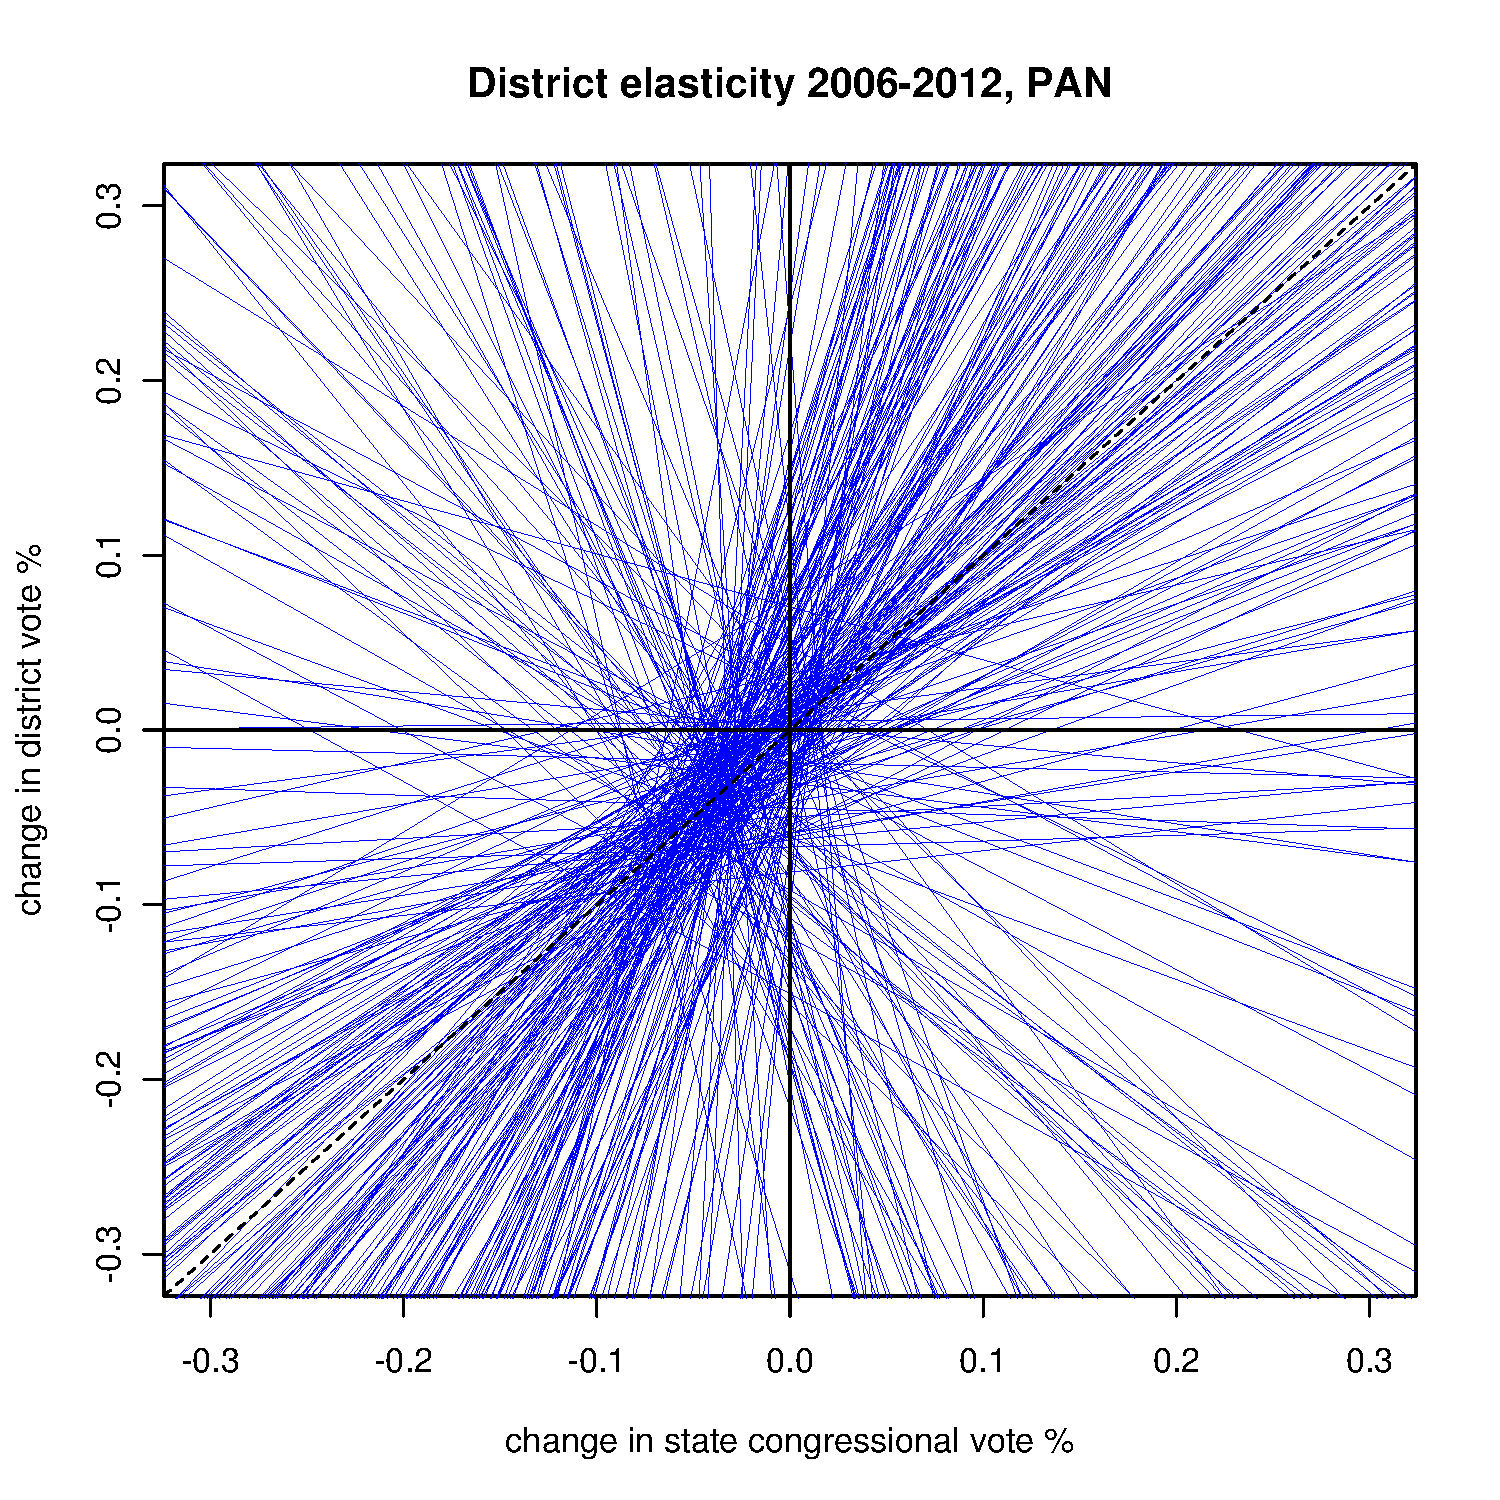
\includegraphics[width=.4\columnwidth]{elastpand0.pdf} & 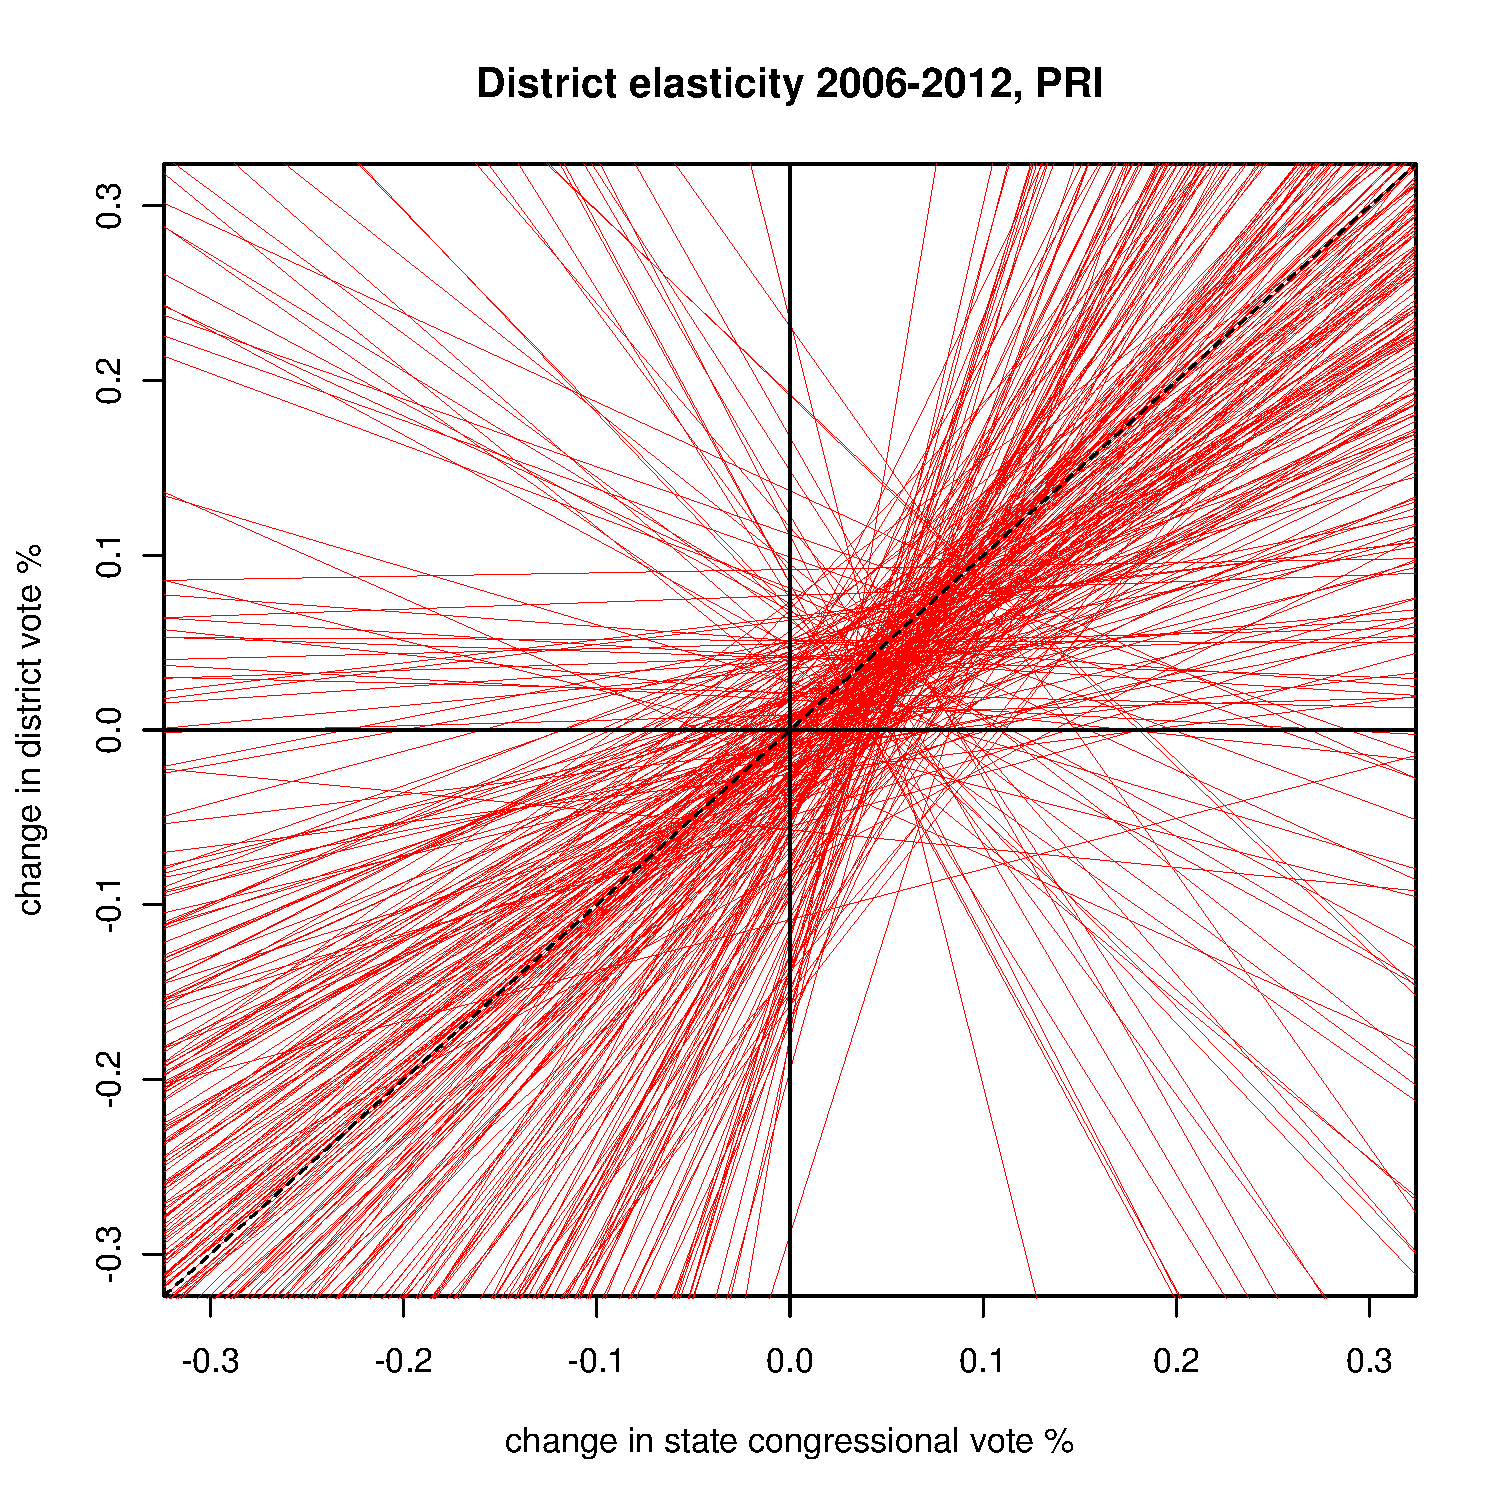
\includegraphics[width=.4\columnwidth]{elastprid0.pdf} \\
    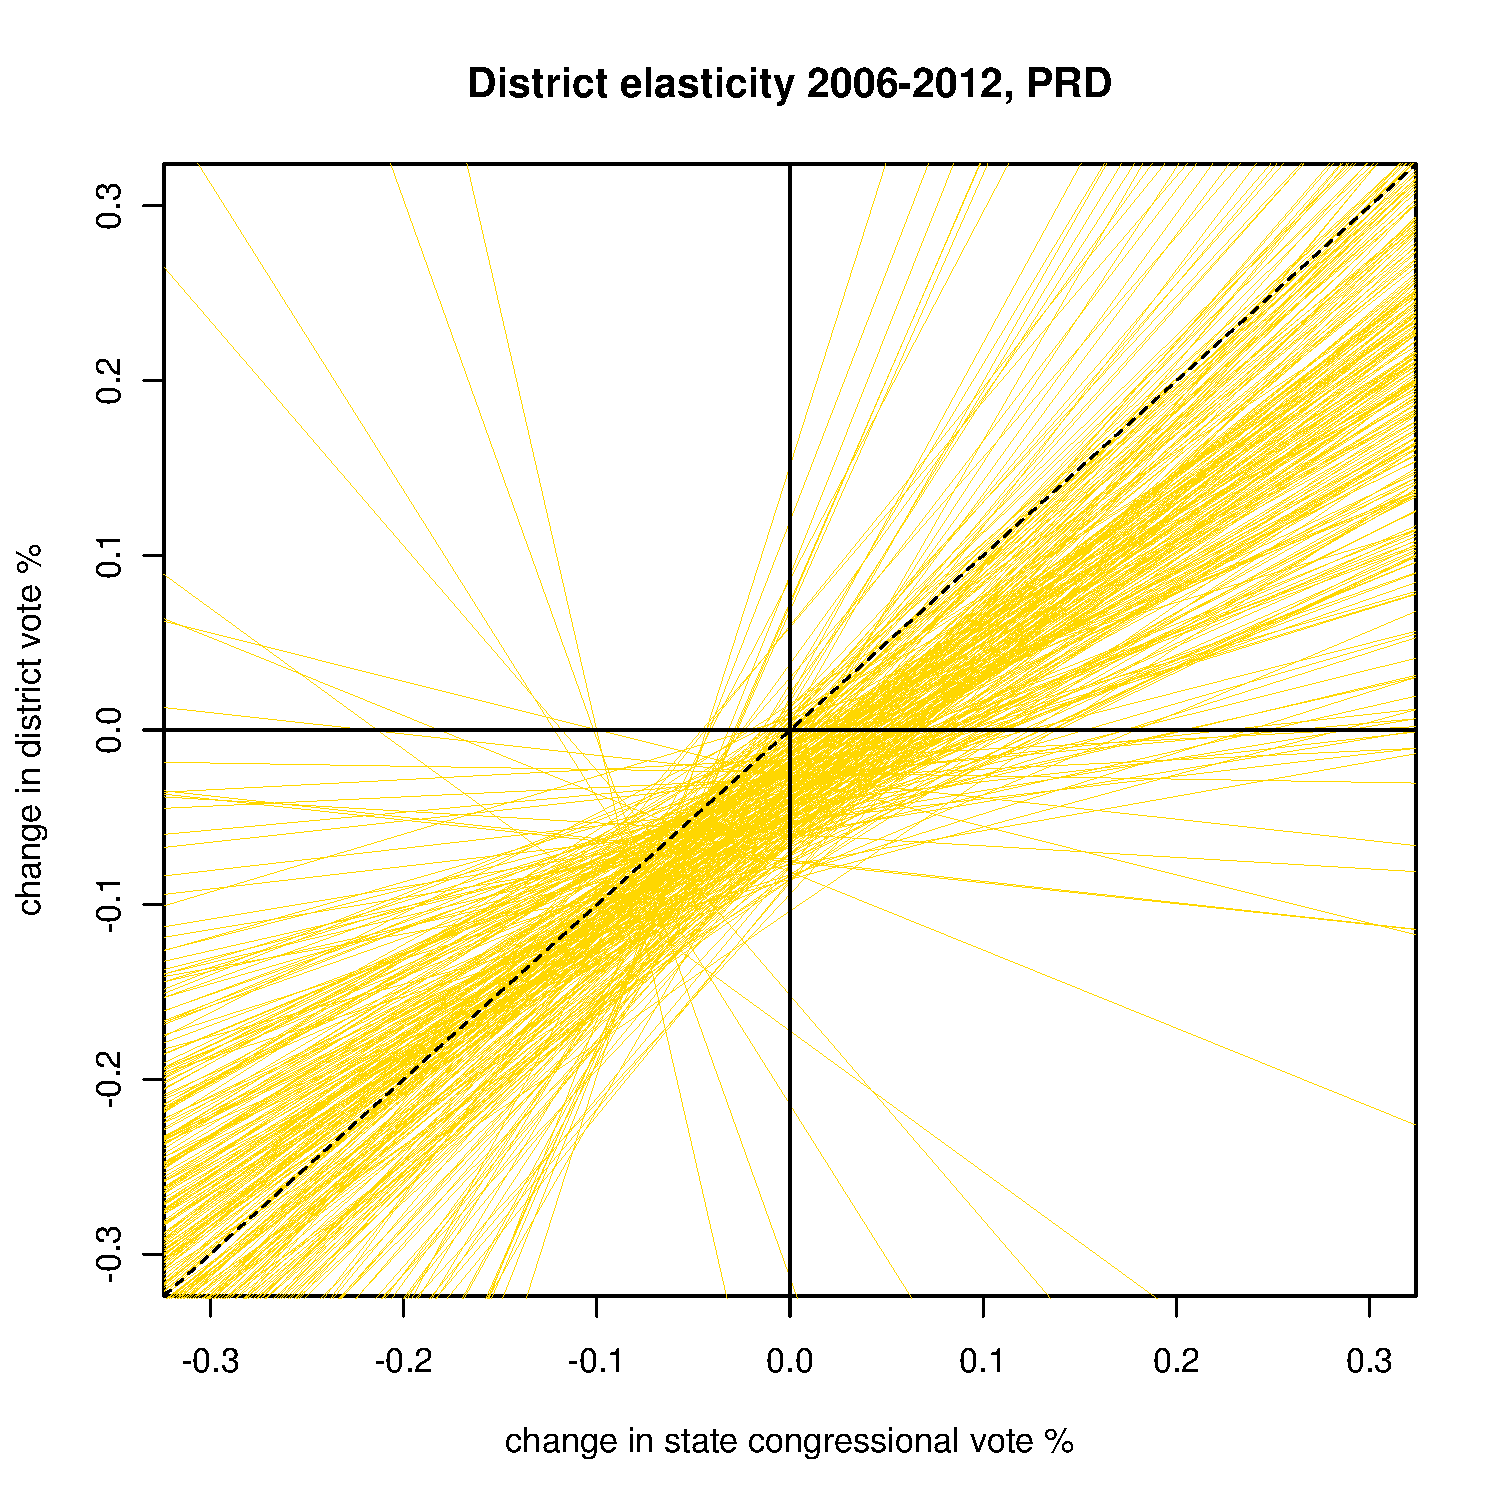
\includegraphics[width=.4\columnwidth]{elastprdd0.pdf} &  \\
  \end{tabular}
  \caption{Parties' district elasticities}\label{F:malmgnat}
\end{center}
\end{figure}



\bibliographystyle{apsr}
\bibliography{../../../../../mydocs/magar}
%\bibliography{bib/magar}



\end{document}
